\documentclass[a4paper, 10pt, twoside]{report}

\usepackage[utf8]{inputenc}
\usepackage[T1]{fontenc}
\usepackage[polish, english]{babel}
\usepackage{todonotes}
\usepackage{float}
\usepackage{booktabs}
\usepackage{multirow}
\usepackage[hidelinks]{hyperref}
\usepackage{titlesec}
\usepackage{amsmath}
\usepackage{amssymb} 
\usepackage{calc} 
\usepackage{graphicx}
\usepackage[noabbrev]{cleveref}
\usepackage[font=small]{caption}
\usepackage{subcaption}
\usepackage{url}
\usepackage{setspace}
\usepackage{acronym}
\usepackage[acronym]{glossaries}
\usepackage[most]{tcolorbox}

% abbreviations
\makeglossaries
\newacronym{ft}{F/T}{Force / Torque}
\newacronym{imu}{IMU}{Inertial Measurement Unit}
\newacronym{mal}{MAL}{Modality Attention Layer}
\newacronym{haptr}{HAPTR}{Haptic Transformer}
\newacronym{lidar}{LiDAR}{Light Detection and Ranging}
\newacronym{ahrs}{AHRS}{Attitude and Heading Reference System}
\newacronym{slam}{SLAM}{Simultaneous Localization and Mapping}
\newacronym{agv}{AGV}{Atomated Guided Vehicle}
\newacronym{cnn}{CNN}{Convolutional Neural Network}
\newacronym{rnn}{RNN}{Recurrent Neural Network}
\newacronym{svm}{SVM}{Support Vector Machine}
\newacronym{dec}{DEC}{Deep Embeddings Clustering}
\newacronym{dof}{DoF}{Degrees of Freedom}
\newacronym{lstm}{LSTM}{Long-Short Term Memory}
\newacronym{bilstm}{Bi-LSTM}{Bidirectional Long-Short Term Memory}
\newacronym{ae}{AE}{Autoencoder}
\newacronym{sae}{SAE}{Stacked Autoencoder}
\newacronym{tsne}{t-SNE}{t-distributed Stochastic Neighbor Embedding}
\newacronym{pca}{PCA}{Principal Component Analysis}
\newacronym{kl}{KL}{Kullback - Leibler}
\newacronym{grf}{GRF}{Ground Reaction Force}
\newacronym{cog}{CoG}{Center of Gravity}
\newacronym{dtw}{DTW}{Dynamic Time Warping}
\newacronym{knn}{KNN}{K Nearest Neighbour}
\newacronym{ee}{EE}{Elastic Ensemble}
\newacronym{cote}{COTE}{Collective of
Transformation-Based Ensembles}
\newacronym{hive}{HIVE}{Hierarchical Voting}
\newacronym{tsc}{TSC}{Time Series Classification}
\newacronym{boss}{BOSS}{Bag-of-SFA Smbols}
\newacronym{rocket}{ROCKET}{Random Convolutional Kernel Transform}
\newacronym{tcn}{TCN}{Temporal Convolutional Network}
\newacronym{putany}{PUTAny}{Poznan University of Technology ANYmal dataset}
\newacronym{qcat}{QCAT}{Queensland Civil and Administrative Tribunal dataset}
\newacronym{pvc}{PVC}{Polivinyl Chloride}
\newacronym{fft}{FFT}{Fast Fourier Transform}
\newacronym{mlp}{MLP}{Multi-Layer Perceptron}
\newacronym{rgb}{RGB}{Red Green Blue}
\newacronym{rgbd}{RGB-D}{Red Green Blue - Depth}
\newacronym{bigs}{BiGS}{BioTac Grasp Stability Dataset}
\newacronym{bigs2}{BiGS V2}{BioTac Grasp Stability Dataset V2}
\newacronym{hatt}{HaTT}{Penn Haptic Texture Toolkit}
\newacronym{phac}{PHAC-2}{Penn Haptic Adjective Corpus 2}
\newacronym{lmf}{LMF}{Low-Rank Multimodal Fusion}
\newacronym{moe}{MoE}{Mixture of Experts}
\newacronym{mid}{Mid}{Intermediate Fusion}
\newacronym{fc}{FC}{Fully Connected}
\newacronym{mae}{MAE}{Mean Absolute Error}
\newacronym{mape}{MAPE}{Mean Absolute Percentage Error}
\newacronym{cpu}{CPU}{Central Processing Unit}
\newacronym{gpu}{GPU}{Graphics Processing Unit}
\newacronym{auc}{AUC}{Area Under Curve}
\newacronym{roc}{ROC}{Receiver Operating Characteristic}
\newacronym{deideo}{DEI-DEO}{Decision In-Decision Out}
\newacronym{fifo}{FIFO}{Feature In-Feature Out}
\newacronym{birch}{BIRCH}{Balanced Iterative Reducing and Clustering using Hierarchies}
\newacronym{svd}{SVD}{Singular Value Decomposition}
\newacronym{eda}{EDA}{Exploratory Data Analysis}
\newacronym{gmm}{GMM}{Gaussian Mixture Model}
\newacronym{em}{EM}{Expectation-Maximization}


% add shortcuts for a formal definition of problems
\usepackage{glossaries}% Shortcuts
\newcommand{\ieee}[1]{(© #1 IEEE)}
\newcommand{\mdpi}[1]{(#1 MDPI)}
\newcommand{\elsevier}[1]{(© #1 ELSEVIER)}
\newcommand{\hide}[1]{}
\newcommand{\Figure}{Fig.~}
\newcommand{\Table}{Tab.~}
\newcommand{\Equation}{Eq.~}
\newcommand{\ie}{{i.e.,~}}
\newcommand{\eg}{{e.g.,~}}
\newcommand{\np}{{np.~}}
\newcommand{\cf}{\emph{cf.~}}
\newcommand{\bdmath}{\begin{dmath}}
\newcommand{\edmath}{\end{dmath}}
\newcommand{\beq}{\begin{equation}}
\newcommand{\eeq}{\end{equation}}
\newcommand{\bdm}{\begin{displaymath}}
\newcommand{\edm}{\end{displaymath}}
\newcommand{\bea}{\begin{eqnarray}}
\newcommand{\eea}{\end{eqnarray}}
\newcommand{\beal}{\beq \begin{array}{ll}}
\newcommand{\eeal}{\end{array} \eeq}
\newcommand{\beas}{\begin{eqnarray*}}
\newcommand{\eeas}{\end{eqnarray*}}
\newcommand{\ba}{\begin{array}}
\newcommand{\ea}{\end{array}}
\newcommand{\bit}{\begin{itemize}}
\newcommand{\eit}{\end{itemize}}
\newcommand{\ben}{\begin{enumerate}}
\newcommand{\een}{\end{enumerate}}

% Groups, Domains, Sets
\newcommand{\SO}{\mathrm{SO}}
\newcommand{\SE}{\mathrm{SE}}
\newcommand{\se}{\mathfrak{se}}
\newcommand{\Real}{\mathbb{R}}
\newcommand{\Int}{\mathbb{Z}}
\newcommand{\ImageDomain}{\Omega}
\newcommand{\Surface}{\mathcal{S}}
\newcommand{\SEtwo}{\ensuremath{\mathrm{SE}(2)}\xspace}
\newcommand{\SEthree}{\ensuremath{\mathrm{SE}(3)}\xspace}
\newcommand{\SOtwo}{\ensuremath{\mathrm{SO}(2)}\xspace}
\newcommand{\SOthree}{\ensuremath{\SO(3)}\xspace}
\newcommand{\sothree}{\ensuremath{\so(3)}\xspace}
\newcommand{\setdef}[2]{ \{#1 \; {:} \; #2 \} }

% Calligraphic fonts
\newcommand{\calA}{{\cal A}}
\newcommand{\calB}{{\cal B}}
\newcommand{\calC}{{\cal C}}
\newcommand{\calD}{{\cal D}}
\newcommand{\calE}{{\cal E}}
\newcommand{\calF}{{\cal F}}
\newcommand{\calG}{{\cal G}}
\newcommand{\calH}{{\cal H}}
\newcommand{\calI}{{\cal I}}
\newcommand{\calJ}{{\cal J}}
\newcommand{\calK}{{\cal K}}
\newcommand{\calL}{{\cal L}}
\newcommand{\calM}{{\cal M}}
\newcommand{\calN}{{\cal N}}
\newcommand{\calO}{{\cal O}}
\newcommand{\calP}{{\cal P}}
\newcommand{\calQ}{{\cal Q}}
\newcommand{\calR}{{\cal R}}
\newcommand{\calS}{{\cal S}}
\newcommand{\calT}{{\cal T}}
\newcommand{\calU}{{\cal U}}
\newcommand{\calV}{{\cal V}}
\newcommand{\calW}{{\cal W}}
\newcommand{\calX}{{\cal X}}
\newcommand{\calZ}{{\cal Z}}

% Image
\newcommand{\Image}{\mathtt{I}}
\newcommand{\Depth}{\mathtt{D}}
\newcommand{\bearingvec}{\mathbf{f}}
\newcommand{\px}{\mathbf{u}} % Pixel
\newcommand{\pt}{\mathbf{p}} % 3D point
\newcommand{\depth}{d}
\newcommand{\proj}{\pi}



% Transformation
\newcommand{\T}{\mathbf{T}}
\newcommand{\R}{\mathbf{R}}
\renewcommand{\S}{\mathtt{S}}
\newcommand{\Identity}{\mathbf{I}}
\newcommand{\inv}{^{-1}}

% Matrices
\newcommand{\trace}[1]{\mathrm{tr}\left(#1\right)}

% Other
\newcommand{\residual}{\mathbf{r}}
\newcommand{\transpose}{\mathsf{T}}
\newcommand{\Zero}{\mathbf{0}}
\newcommand{\eye}{{\mathbf I}}
\renewcommand{\skew}{{\mathbf S}}
\newcommand{\Jac}{\mathtt{J}}
\newcommand{\Zthree}{\Zero_{3 \times 3}}
\newcommand{\Ithree}{\eye_{3 \times 3}}

% Imu
\newcommand{\rotvel}{\omega}
\newcommand{\acc}{a}
\newcommand{\rotvec}{\boldsymbol\phi}
\newcommand{\rotvecpert}{\delta\rotvec}
\newcommand{\rotvecang}{\varphi}	% rotation vector angle
\newcommand{\rotvecdir}{\mathbf{a}} % rotation vector direction
\newcommand{\tran}{\mathbf{p}}
\newcommand{\tranpert}{\delta\tran}
\newcommand{\vel}{\mathbf{v}}
\newcommand{\velpert}{\delta\vel}
\newcommand{\bias}{\mathbf{b}}
\newcommand{\biaspert}{\delta\bias}
\newcommand{\gravity}{\mathbf{g}}
\newcommand{\noise}{\boldsymbol\eta}
\newcommand{\VIO}{VIO\xspace}
\newcommand{\odometry}{navigation\xspace}
\newcommand{\tango}{{\rm Tango}\xspace}

% Paper Specific
\newcommand{\Cov}{\mathbf{\Sigma}}
\newcommand{\at}[1]{^{(#1)}}
\newcommand{\expmap}{\mathrm{Exp}}
\newcommand{\logmap}{\mathrm{Log}}
\newcommand{\normsq}[2]{\left\|#1\right\|^2_{#2}}
\renewcommand{\d}{\text{d}}
\newcommand{\Rmean}{\R}
\newcommand{\Rrand}{\tilde\R}
\newcommand{\eq}{Eq.}
\newcommand{\eqs}{Eqs.}

\newcommand{\iSAMtwo}{iSAM2\xspace}
\newcommand{\MAP}{MAP\xspace}
\newcommand{\SVO}{SVO\xspace}
\newcommand{\GN}{GN\xspace}
\newcommand{\States}{\mathcal{X}}
\newcommand{\State}{\boldsymbol{x}}
\newcommand{\meascam}{\mathcal{C}}
\newcommand{\measimu}{\mathcal{I}}
\newcommand{\covprior}{\mathbf{\Sigma}}
\newcommand{\covimu}{\mathbf{\Sigma}}
\newcommand{\covcam}{\mathbf{\Sigma}_{\meascam}}
\newcommand{\World}{\mathtt{W}}
\newcommand{\Imu}{\mathtt{I}}
\newcommand{\Camera}{\mathtt{C}}
\newcommand{\world}{\mathtt{{W}}}
\newcommand{\landmarkfr}{\text{{L}}}
\newcommand{\Landmarkfr}{\text{{L}}}
\newcommand{\imu}{\mathtt{{I}}}
\newcommand{\base}{\mathtt{{B}}}
\newcommand{\contact}{\mathtt{{K}}}
\newcommand{\Base}{\mathtt{{B}}}
\newcommand{\camera}{\mathtt{C}}
\newcommand{\foot}{\mathtt{K}}
\newcommand{\cam}{{\scriptsize \text{c}}}
\newcommand{\accshort}{\tilde\acc(t)\!-\! \bias^a(t) \!-\! \noise^{ad}(t)}
\newcommand{\preintVar}{increments\xspace} 
\newcommand{\biasFixedPreintVar}{bias-fixed increments\xspace} 
\newcommand{\biasFixed}{\bar{\bias}}
\newcommand{\biasFixedDelta}{\Delta}
\newcommand{\biasHat}{\hat{\bias}}
\newcommand{\meters}{\rm{m}}
\newcommand{\preintRmeas}{\Delta\tilde\R}
\newcommand{\preintVmeas}{\Delta\tilde\vel}
\newcommand{\preintPmeas}{\Delta\tilde\tran}

% smart factors
\newcommand{\pixel}{\mathbf{z}}
\newcommand{\pixelnoise}{\noise_{cam}}
\newcommand{\landmark}{\mathbf{m}}
\newcommand{\landpert}{\delta\landmark}
\newcommand{\posepert}{\delta\mathbf{T}}
\newcommand{\bvec}{\mathbf{b}}
\newcommand{\Amat}{\mathbf{A}}
\newcommand{\Bmat}{\mathbf{B}}
\newcommand{\Fmat}{\mathbf{F}}
\newcommand{\Emat}{\mathbf{E}}
\newcommand{\Qmat}{\mathbf{Q}}
%
\newcommand{\appendixRef}{Appendix\xspace}
\newcommand{\subimu}{{ij}} 
\newcommand{\indmeas}{(i,j)} 


% Jacobians
\newcommand{\DLog}{\mathtt{J}_{r}^{-1}} 
\newcommand{\DExp}{\mathtt{J}_{r}} 
\newcommand{\DExpk}{\mathtt{J}^k_{r}} 
\newcommand{\jacobian}[2]{\frac{\partial #1}{\partial #2}}

% updates
\newcommand{\rup}{\rotvecpert} 
\newcommand{\tup}{\tranpert} 
\newcommand{\vup}{\velpert} 
\newcommand{\bupa}{\tilde\delta{\bias^a_i}} 
\newcommand{\bupg}{\tilde\delta{\bias^g_i}}

% Preintegrated measurements
\newcommand{\pRot}{\Delta\bar\R_{ij} } % integration value
\newcommand{\pRotk}{\Delta\bar\R_{ik} } % integration value
\newcommand{\pTran}{\Delta\bar\tran_{ij}}
\newcommand{\pVel}{\Delta\bar\vel_{ij}}
\newcommand{\pVelk}{\Delta\bar\vel_{ik}}
\newcommand{\mRot}{\Delta\tilde\R_{ij}} % measured
\newcommand{\mTran}{\Delta\tilde\tran_{ij}}
\newcommand{\mVel}{\Delta\tilde\vel_{ij}}
\newcommand{\Adjoint}{\mathtt{Ad}}

\newcommand{\biasCorrectedGyroMeas}{\tilde\rotvel(t) \!-\! \bias^g(t)}
\newcommand{\biasCorrectedAccMeas}{\tilde\acc(t) \!-\! \bias^a(t)}
\newcommand{\Rmeas}{\tilde\R}
\newcommand{\vmeas}{\tilde\vel}
\newcommand{\tmeas}{\tilde\tran}

\newcommand{\w}{\omega}
\newcommand{\wb}{\boldsymbol{\w}}
\newcommand{\bv} {\bias^v}
\newcommand{\bw} {\bias^\omega}
\newcommand{\bvk}{\bias^v_k}
\newcommand{\bwk}{\bias^\omega_k}
\newcommand{\bvi}{\bias^v_i}
\newcommand{\bwi}{\bias^\omega_i}
\newcommand{\debias}{\delta \bias}
\newcommand{\debiasv}{\delta \bv}
\newcommand{\pbias}{\partial \bias}

\newcommand{\etab}{\boldsymbol{\eta}}
\newcommand{\etabij}{\etab_{ij}}
\newcommand{\etav}{\etab^v}
\newcommand{\etavk}{\etab^v_k}
\newcommand{\etaw}{\etab^\omega}
\newcommand{\etavd}{\etab^{v d}}
\newcommand{\etawd}{\etab^{\w d}}
\newcommand{\etavdk}{\etab^{v d}_k}
\newcommand{\etawdk}{\etab^{\w d}_k}


\newcommand{\tp}{\tilde{\tran}}
\newcommand{\tv}{\tilde{\vel}}
\newcommand{\tw}{\tilde{\wb}}
\newcommand{\tR}{\tilde{\R}}
\newcommand{\tvk}{\tilde{\vel}_k}
\newcommand{\twk}{\tilde{\rotvel}_k}

\newcommand{\dP}{\Delta \tran}
\newcommand{\dep}{\delta \tran}
\newcommand{\depij}{\dep_{ij}}
\newcommand{\depik}{\dep_{ik}}
\newcommand{\dpij}{\Delta \tran_{ij}}
\newcommand{\dRij}{\Delta \R_{ij}}
\newcommand{\dRik}{\Delta \R_{ik}}
\newcommand{\dPhi}{\delta \rotvec}
\newcommand{\dt}{\Delta t}
\newcommand{\dR}{\Delta \R}
\newcommand{\dtp}{\Delta\tilde{\tran}}
\newcommand{\dtR}{\Delta\tilde{\R}}
\newcommand{\dtRij}{\Delta\tilde{\R}_{ij}}
\newcommand{\dtRik}{\Delta\tilde{\R}_{ik}}
\newcommand{\dtpij}{\Delta\tilde{\tran}_{ij}}
\newcommand{\dtpik}{\Delta\tilde{\tran}_{ik}}
\newcommand{\dbvij}{\Delta\bv_{ij}}
\newcommand{\dbwij}{\Delta\bw_{ij}}
\newcommand{\dPhiij}{\delta\rotvec_{ij}}
\newcommand{\dPhiik}{\delta\rotvec_{ik}}

\newcommand{\sumjmo} [1]{\sum_{k=i}^{j-1}\left[ #1 \right]}
\newcommand{\sumjmt} [1]{\sum_{k=i}^{j-2}\left[ #1 \right]}
\newcommand{\prodjmo}[1]{\prod_{k=i}^{j-1}\left[ #1 \right]}
\newcommand{\prodjmt}[1]{\prod_{k=i}^{j-2}\left[ #1 \right]}
\newcommand{\Exp}[1]{\expmap \left( #1 \right)}
\newcommand{\Log}[1]{\logmap \left( #1 \right)}

\newcommand{\Jrk}{J_r^k}
\newcommand{\defeq}{\triangleq}


\newtcolorbox{notefromauthor}[1][]{%
    colback=black!5,
    colframe=black!5,
    notitle,
    sharp corners,
    borderline west={2pt}{0pt}{red!80!black},
    enhanced,
    breakable,
    fontupper=\linespread{.9}\selectfont
    }


\title{Combining interaction and perception to determine the physical properties of the robot environment}

\author{Michał Bednarek}

\begin{document}

\maketitle
\setstretch{1.3}
\tableofcontents

\chapter*{Abstract}
\label{sec:abstract}

The number of autonomous robot use cases significantly increased in multiple real-life scenarios, \eg autonomous vehicles for transportation, safety and security, industrial inspection, or even space exploration. These are only a few examples from the plethora of new, inspiring, challenging domains where manipulators or mobile robots, \eg walking machines, can be utilized. The real-life robotic use cases require robust perception, an intersection of sensor mechanics, hardware, and multi-modal data processing. Managing this complex system is often not trivial. Nevertheless, with autonomy comes responsibility and increasing demand for understanding the environment around an agent. The robot must adapt to unpredictable situations and cope with the open-world assumption. In this thesis, I advocate that the perception system robustness might be achieved by exploiting the haptic properties of the surroundings. There is a pressing need to explore this topic as the current solutions must cope better with this modality.

The following dissertation aims to create a unified robotic perception system that would meet the requirements of real-world applications and deliver appropriate information for onboard robot systems, \eg localization, obstacle avoidance, or manipulation. Such a perception system has to be low-cost and computationally low-demanding due to the limited resources available on a mobile robot. A methodology concerns artificial intelligence, especially machine learning. These methods dominated the field of perception in recent years due to their superior performance, and their choice was natural. Deep learning methods focus predominantly on a supervised setup in material/terrain classification or when a continuous variable associated with a specific parameter is needed (\eg stiffness estimation). Moreover, I also explored an unsupervised learning setup as it became a fundamental tool for understanding hidden characteristics in sensory data. Eventually, perception robustness emerged as a crucial characteristic of deploying it in the real world. The dissertation includes multiple solutions to increase the robustness, primarily by using attention modules.

\chapter*{Streszczenie}
\label{sec:streszczenie}

\begin{otherlanguage}{polish}
Percepcja robotyczna jest intensywnie rozwijającą się dziedziną, leżącą na styku sprzętu, mechaniki i wielomodalnego przetwarzania danych, które często nie są łatwe do wykorzystania. Można zaobserwować, że liczba autonomicznych robotów znacznie wzrosła w wielu dziedzinach życia, takich jak autonomiczne pojazdy transportowe, bezpieczeństwo, inspekcja przemysłowa czy nawet eksploracja kosmosu. To tylko kilka przykładów z mnóstwa nowych, inspirujących, ale wymagających dziedzin, w których roboty będą wykorzystywane do manipulacji i przemieszczania się. Niemniej z autonomią wiąże się pewna odpowiedzialność i rosnące zapotrzebowanie na zrozumienie środowiska otaczającego robotycznego agenta, tak aby mógł się dostosować do {nieprzewidywalnych} sytuacji. Obecnie systemy percepcji jedynie w niewielkim stopniu rozpoznają właściwości taktylne otoczenia. 

Celem rozprawy jest stworzenie systemu percepcji robotycznej, który spełniałby wymagania rzeczywistych zastosowań i dostarczał informacje dla systemów działających na pokładzie, takich jak lokalizacja, unikanie przeszkód czy strategia manipulacji. Ponadto, system musi być tani i mało wymagający obliczeniowo ze względu na ograniczone zasoby robota mobilnego. Metodyka pracy dotyczy przede wszystkim sztucznej inteligencji, a zwłaszcza uczenia maszynowego. Metody te zdominowały tę dziedzinę ze względu na najlepsze wyniki, więc ich wybór był naturalny. W niniejszej rozprawie przedstawione zostały metody głębokiego uczenia nadzorowanego w dwóch typach zadań. Po pierwsze w klasyfikacji powierzchni dotykanej przez robota. Po drugie w zadaniu regresji parametrów fizycznych tejże powierzchni, do których zalicza się np. sztywność dotykanego obiektu. Uczenie nienadzorowane natomiast jest kluczowym narzędziem do zrozumienia ukrytych właściwości danych sensorycznych oraz tego, jak robot może je wykorzystać bez nadzoru. Także odporność percepcji robota okazała się ważną cechą dla wdrożenia systemu w rzeczywistości. Poniższa rozprawa zawiera rozwiązania mające na celu jej zwiększenie, głównie poprzez wykorzystanie modułów atencji.
\end{otherlanguage}

\chapter*{Acknowledgments}
\label{sec:acknowledgements}

I want to take this opportunity to express my sincere gratitude to many people who have been instrumental in my journey toward completing this Ph.D. thesis.

First and foremost, I would like to thank my auxiliary Ph.D. supervisor, Krzysztof Walas, for his long-term cooperation in research projects, scientific work, opportunities to visit the best places to grow as a researcher, and his unwavering support during the tough times. I would also like to express my sincere appreciation to my other Ph.D. supervisor, Paweł Drapikowski, for his guidance throughout the process of writing this thesis, his invaluable reviews, and his kind words of encouragement.

I want to acknowledge the tremendous contributions to the work of my co-authors of my research papers and other colleagues at the Institute of Robotics and Machine Intelligence, who have provided me with a stimulating research environment and countless opportunities to collaborate and learn. With fruitful discussions, brainstorming, and endless conversations with you on various topics, that work would be complete with the conclusions drawn during them.

Lastly, I am deeply grateful to my family, especially my wife, who has always been by my side. Thank you for your unwavering support, understanding, and encouragement throughout this challenging journey. Your love and support have been a constant source of strength and inspiration for me.

\printglossary[title=Abbreviations, type=\acronymtype,style=long,nonumberlist]

\chapter*{Content}
\label{sec:content}

Chapters~\ref{part:methods:materials} and~\ref{part:methods:terrain} present tactile and kinesthetic sensing solutions for robotic arms and walking robots. In both robotic setups, an agent interacted with a nondeterministic environment, such as deformable objects or rough terrains with different material classes. All developed perception systems are based on deep learning methods. When writing this thesis, they achieved state-of-the-art classification, recognition, and representation of learning results. Methods for material classification and object stiffness regression using a soft gripper~\cite{MIT3fingerGripper} were taken on in Chapter~\ref{part:methods:materials}. Moreover, this Chapter also investigates the unsupervised learning approach for haptic data grouping without supervision. This task is an emerging topic in the robotics community and a way to tackle learning from the tremendous amount of available datasets without the manual labelling process, which is time-consuming, expensive, and tedious. Chapter~\ref{part:methods:terrain} presents the research conducted in the walking robots area, including the classification of terrains using \acrshort{ft} sensors feedback or orientation provided by the \acrshort{imu}. All experiments in this Chapter were performed with a high emphasis on generalization for different robots and rapid inference time. That Chapter also presents the \acrfull{mal} as a solution for the weighting input modalities concerning their \textit{significance} level, which results in improvements in a system's robustness against input data degradation. Chapter~\ref{part:methods:terrain} presents the multi-modal fusion methods using deep learning. Multiple state-of-the-art predictive models were tested on three, separate datasets prepared for different robotic, perception-related tasks -- manipulation of deformable objects~\cite{bigs}, texture recognition~\cite{penn_haptix}, and multi-label classification of haptic adjectives~\cite{haptic_from_vision_and_biotac}. These datasets include time-series data from different (often non-homogeneous) modalities, \eg video streams, and \acrfull{ft} sensors, where it is not a trivial task to couple them together. The work tackled the problem of multi-modal fusion by measuring the overall performance of different deep neural networks in the selected tasks. Moreover, the research includes examining the impact of sensor failures and noise in the input data on the final results -- looking at the problem from the robotics perspective. The results from this work gave a highly valued insight into the fusion of different modalities in the data-driven approaches to robotic tasks.

Chapters in Part~\ref{part:experiments} contain experimental verification of developed/adapted methods. Chapter~\ref{part:experiments:materials} shows the comparison of different approaches to the object's stiffness estimation using a simulated dataset and real-world data samples. It focuses on the \acrfull{rnn} and the number of real-world data samples included in the simulation dataset to fill in the \textit{reality gap} -- a common phenomenon present in data-driven approaches trained in the simulated environments. Moreover, the experiments towards unsupervised learning utilized the \acrfull{dec} method~\cite{DEC}. Chapter~\ref{part:experiments:terrain} presents the \acrfull{haptr} - a novel and lightweight approach that utilizes attention modules to classify the terrain samples based on haptic/inertial time series. In the following work, the \acrshort{haptr} was compared to state-of-the-art algorithms and achieved high performance in this task. Chapter~\ref{part:experiments:fusion} presents an extensive comparison of multi-modal fusion methods -- Late Fusion, \acrfull{moe}, \acrfull{mid}, and \acrfull{lmf}, with an emphasis on the significance of the feature level fusion and data degradation robustness. 

In Chapter~\ref{part:conclusions} final remarks were given, a summary with discussion on results and plans for future research. All chapters in the following dissertation include a domain-specific literature review.

% description of my work (also for non-technician people)
\part{Introduction}
\label{part:introduction}

\chapter{Motivation}
\label{part:introduction:motivation}

\section{Broad perspective}
\label{part:introduction:motivation:perspective}

% more and more applications of mobile and ground robots
In the coming years, we will observe a rapidly growing market for ground robots that can operate in many different environments. The idea that mobile robots could assist humans in various tasks started penetrating people's awareness. Many factors influence the development of advanced robotics systems. Firstly, we have a global viewpoint based on the competition between countries, research facilities, or commercial companies and the market's response to that phenomenon. Secondly, the scientific perspective -- seen as the progress in robotics perception research, inspires more and more people to be engaged in that competition.

% Global perspective - why is robotics perception so important for large players?
Nowadays, large companies compete in the high-tech industry, accelerating the development of robotic innovations. Anybotics's ANYmal~\cite{anymal} or Boston Dynamics' Spot are great examples of mobile robots' maturity, and we can expect that they will soon be deployed in significant numbers. From a global standpoint, innovations create new markets and supply chains. That, in turn, improves the strategic position of a facility that controls a new technology. Let the development of the space industry be an example. For many years wheeled robots (\eg lunar rovers) served different space agencies in their missions to gather new information about planets in the Solar System. However, there is still no autonomous system capable of exploring, e.g., steeper slopes -- crucial places from the geological point of view. Wheeled systems are unprepared to adapt well enough to rough, inclined and unpredictable terrain. However, the answer to that problem would be a legged platform such as~\cite{spacebok} that interacts with its environment and could adapt its gait to the unpredictable ground surface.

Additionally, such a robot should also autonomously recover from any fall. Its perception system should properly recognize terrain properties using all the available sensory information. Even if there is a limited demand for this type of system right now, with great confidence, it will appear in the coming years. One can observe the increasing competition between global, high-tech players in space exploration. The company that will provide such a solution will make a tangible profit in the future, creating commercial potential for developing robotics perception systems.

% Scientific perspective - why robotics perception is so important for researchers and regular people?
On the other hand, the rapid development of robotic perception systems can also be more down-to-earth. Firstly, sensors have become more affordable in recent years, which has engaged more and more research groups in the field. It is a scientific breakthrough because of the popularity of advanced sensory systems, \eg \acrshort{ft} measurement devices, \acrfull{lidar} scanners, 2D laser scanners, depth cameras, or a variety of inertial sensors such as \acrfull{imu} or more sophisticated \acrfull{ahrs}. All of them pushed forward the pace at which new technologies in robotics appeared over the last few years. Innovations in sensory systems and the increasing computational power of modern processing units brought an opportunity to apply existing algorithms in the real world, find their limitations, and improve or replace them with new ones. 

A robust robotic perception became an emerging field at the level of governments and corporations creating the global market. Additionally, the accessibility to the knowledge and required hardware started to be relatively easy. Taking both factors into account, the author of the following dissertation believes that now is the right time to pursue research in that topic -- \textit{it is not too early, nor too late}~\footnote{Panel \textit{How to be a Good Citizen of the CVPR Community} -- a talk by Vladen Koltun.}.

% We have a broad picture of why robotics perception is essential. So, what is the question that arises from that problem?
Information about a robot's environment is crucial when developing a robust system that would let a robot autonomously adapt to the current circumstances or explore undiscovered knowledge. Nowadays, robots utilize geometric information about its surrounding, and they use camera images, depth maps, or point clouds -- namely visual sources. Multiple research areas use these sources of visual information, like \acrfull{slam}, path planning, obstacle avoidance, scene reconstruction, or manipulation of elastic objects. Until the robotic agent's surroundings are static, rigid, and predictive, the perception problem might be solvable without any high-level understanding. Nowadays, many semi-autonomous machines operating in highly controlled environments use only geometric information about a scene. A great example of such applications is an \acrfull{agv} used chiefly in logistics and can successfully navigate in 2D maps using laser scanners. However, such robots are prone to errors whenever their environment stops being static, \eg when the human enters the zone or a hall's arrangement changes. Taking such cases into account, recently, more and more researchers have noticed that the environment's geometry is not enough to achieve a robust perception, especially when considering the deployment of a robot in the human world. A high-level understanding also matters and is vital to the perception system. Understanding the semantics of the scene is crucial to interact with it because it gives the cues if the robot can complete the task and, if so -- how to behave or interact with the environment to complete a mission.

\section{Problem statement}
\label{part:introduction:problem}

The robotic agent must have some internal representation of the world around it to adapt to and overcome environmental conditions -- the notion of physical properties as a mass, friction, stiffness, or more categorical, \eg a class of an object or a surface. However, it is challenging to provide such representation, as mobile robots operate in unstructured and often unpredictable environments, and their perception systems must handle many disturbances. Data-driven methods are the most popular yet most effective approaches for representation learning. Typically, they operate on learnable features where the recognition task is more facilitated than using raw sensory feedback. Nevertheless, they suffer from multiple drawbacks. Firstly, they require a vast amount of data to generalize. For example, the terrain recognition system trained on the dataset with samples gathered only on the flat surface probably will not be fully operational when slopes appear. Secondly, the noise in the training data might mislead the perception system and turn the training process into overfitting or being sensitive to sample-specific glitches. The thesis's main objective is to explore and implement a system composed of functional blocks that would enable and further improve the overall quality of robotic haptic sensing. The goals of this dissertation allowed for the formulation of scientific theses, which gave a present shape to this work:

\textbf{Haptic robotic perception, defined as a capability of a robotic agent to recognize complex patterns in tactile and kinesthetic sensations, can be achieved using deep learning methods because they exhibit superior performance in a vast majority of automated tasks. That ability can be further extended by unsupervised learning methods that let analyze the incoming data and measure its similarity to previously seen examples, which improves a high-level understanding of the robot's environment.}

The supporting theses follow the statement of this dissertation that refer to particular gains brought to the robust perception system as a result of this research:

\begin{itemize}  
    \item Typically, haptic signals are time-series, \eg forces, torques, or inertial measurements representing the motion of a sensor in space. Posing the problem of haptic perception as a sequence-to-sequence task would enable us to use an attention mechanism that produces weights for each sample in the input signal. Feeding such weighted signals to a supervised learning method would simplify the task of, \eg terrain classification and improve the robustness of a proposed system. Such a classifier could focus more on relevant parts of its input.
    
    \item An understanding of the robot’s environment will improve based on the information from multiple modalities, \eg \acrshort{ft} signals, images, or raw sensory signals from haptic electrodes. We can fuse data from heterogeneous modalities using deep learning methods, which do not restrict the proposed system to homogeneous data only.

\end{itemize}

\begin{notefromauthor}
    Chapters of the following dissertation present the author's research contributions, most of which have already appeared in peer-reviewed scientific journals and conferences from 2019 to 2022. Every Chapter includes a heading with listed publications that served as a base for the presented work. The copyright sign with the year of publishing, \eg\elsevier{2019 - 2022}, stands next to published graphics and tables if the publisher's policy requires that for reusing for non-commercial purposes such as including in a dissertation.
\end{notefromauthor}

\part{Methods}
\label{part:methods}

\chapter{Material recognition}
\label{part:methods:materials}

\begin{notefromauthor}
    The following Chapter and the corresponding results in Part~\ref{part:experiments} are partially based on two publications of the author of this thesis. 
    
    \begin{itemize}
        \item \ieee{2019} J. Bednarek, M. Bednarek, P. Kicki, K. Walas (2019) "Robotic Touch: Classification of Materials for Manipulation and Walking". In: IEEE International Conference on Soft Robotics (RoboSoft)
        
        \item M. Bednarek, P. Kicki, J. Bednarek, K. Walas (2021) "Gaining a Sense of Touch Object Stiffness Estimation Using a Soft Gripper and Neural Networks" in Electronics Journal
        
    \end{itemize}
\end{notefromauthor}

\section{Introduction}
\label{part:methods:materials:introduction}

Human perception of the world highly depends on its physics. Our sensory system provides haptic sensations to the brain, which lets us, \eg plan a direct trajectory to grab a cup of tea, squeeze a wet sponge or flip a book page. We know how to do these things and predict objects' deformations based on their physical properties. Moreover, our hands constitute highly effective grippers, outperforming industrial ones in dexterity. Taking into account our assumptions about the world that come from our minds, combined with the \textit{embodied intelligence}~\cite{IIda07} of our hands, we can perfectly adjust the manipulation process to varying external conditions. However, machines do not have such in-built proficiency, and their abilities to manipulate allow only for managing repetitive tasks. 

Soft robotics is a sub-field of robotics that focuses on robot design, its locomotion, and real-world interaction with the environment utilizing 
a paradigm known as the \textit{intelligence by mechanics}~\cite{IIda07}. It assumes that the robot's body should adapt to the surroundings through decentralized mechanical system-environment interactions rather than one decision-making unit, e.g., an artificial neural network. The aftermath of the research on this topic is biologically inspired soft grippers~\cite{YaleOpenHand, MIT3fingerGripper, MITorigamiGripper, LaschiGripper}, designed from soft materials in such a way that can adjust their shape to the grasped objects, which allows them manipulating delicate and deformable objects. One can state that the shape of that gripper corresponds to the physical properties (\eg stiffness, elasticity, roughness) of grasped objects. However, these soft grippers are sensorless by design, and measuring their deformations was not the researcher's area of interest. 

On the one hand, one can observe the growing number of available applications of sensors capable of capturing high-dimensional deformations of soft and unpredictable physical objects~\cite{BatchFabricationSensor, TactileTwo, Realmuto}. However, they do not directly measure the behavior of the soft gripper, but only the properties of the surroundings or grasped objects. In the following dissertation, I argue that we can use traditional and widespread sensors based on microelectromechanical systems to predict the physical nature of the robot's surroundings by estimating the gripper deformation. Thereby, the following chapter presents findings about a supervised, hybrid approach that connects an \textit{embodied intelligence} of a soft gripper with an \textit{artificial intelligence} system to provide an easy-to-use, open-source and inexpensive method of estimating the physical properties of objects with various stiffness parameters. 

The sensors used in material classification are primarily accelerometers~\cite{Strese2014AClassification}, pressure mapping sensors~\cite{Tulbure2018}, 3D force~\cite{Kerzel2017} and 6D \acrshort{ft} sensors~\cite{KubaRNN}. Most approaches presented in the literature use very controlled environments when performing experiments, as in the case of accelerometers~\cite{Strese2014AClassification}. Currently, a preferred approach to material recognition is by a programmed set of exploratory movements instead of a single touch~\cite{Kerzel2017, Tulbure2018}. However, the desired behavior is to achieve a high material classification score in an uncontrolled environment during a normal robot operation without performing particular movements. The classification should be on the raw signals without additional pre-processing and hand-crafted representation. 

As machine learning methods became more accessible to most researchers, these learning-based methods constituted a typical way to improve advancements in particular domains. However, some might argue that embodied intelligence will follow that trend, as it was usually outside the scope of mainstream research topics~\cite{Roy2021}. Robotics is a unique field that almost always requires some form of interaction with the agent's environment, which might prevent unlimited usage of data-driven methods, which happened in other areas related to, \eg computer vision or natural language processing. While the autonomous robot should also operate in unknown environments, another limitation of learning-based algorithms is their need for adaptation to previously unseen scenarios. This restriction leads to the limited capability of real-world deployment except for a narrow set of fields. Yet, there is no simple answer to these problems because no autonomous machine can be prepared for every event. The author of the following thesis argues that we should not try to be ready but actively adapt to changing conditions. In such a setup, unsupervised learning might improve that high-level understanding of the robot environment, where the haptic recognition of materials is a good starting point. There needs to be more research on robot environment understanding using unsupervised learning methods. 

The following chapter investigates multiple approaches to the material and object recognition task. The stiffness estimation problem was tackled using various deep learning methods, including convolutional and recurrent architectures. Moreover, the chapter presents novel haptic datasets for the stiffness estimation based on real-world and simulated \acrshort{imu} signals from sensors attached to the fingers of an elastic gripper. Secondly, the author of the following thesis delved into the challenging problem of unsupervised learning for the haptic recognition task, where the clustering model did not have any prior knowledge about input signals. Typically, these algorithms analyze unlabeled datasets to group them and discover hidden patterns. In robotics, such systems would substantially improve data association of previously seen places, objects, or finding anomalies. However, scientific publications in that field with real-world robotic setups are still limited, even though unsupervised learning is an emerging field of Artificial Intelligence.

\section{Related work}
\label{part:methods:materials:rw}

\subsection{Stiffness measurement}
\label{part:methods:materials:rw:measurements}

In~\cite{rails}, authors proposed a practical application for a continuous rail rigidity measurement using the accelerometer and oscillating mass on the rolling wheel. This work indicates that the issue under examination is vital in engineering. Unlike the previous method, the authors of~\cite{noncontact_stiff} propose to use the non-contact measurement of spindle stiffness. The authors suggested a magnetic loading device that enabled them to make measurements while the spindle rotated. Due to the usage of magnetic loading, that method limits itself to ferromagnetic objects. Measuring a stiffness was also possible at a much smaller scale than presented in~\cite{nano}. The authors reviewed the nanoindentation continuous stiffness measurement techniques and applications. The range of stiffness coefficients of materials is extensive. To avoid saturation and enhance precision, the authors of~\cite{stiff_measurement_system} proposed a portable measurement device able to adjust a sensing range by manipulating tool parameters, such as touch module separation, indenter protrusion, and spring constant of the force sensing module. Authors of~\cite{foams, foams2} analyzed the stiffness measurement techniques applied to the polymer foams, which are similar to those used in this paper. In~\cite{foams} there, was proposed a procedure for measuring stiffness using dot markers on object surfaces and compression plates to exert a force on an object. Authors stressed that non-axial compression tests resulted in worse performance, which was usually the case in robotic manipulation. Similar to the proposed solution, in~\cite{pisa_hand_imu_justification}, authors proposed the \acrshort{imu}-based approach. However, in a different task -- the reconstruction of the configuration of a soft gripper. As opposed to that work, the experimental section of this thesis describes the proposed indirect measurements of the object's stiffness property by the change of behavior of the soft gripper while squeezing, not the gripper's configuration itself.

\subsection{Stiffness estimation}
\label{part:methods:materials:rw:estimation}

The work~\cite{stiff_from_force} presents an alternative approach that does not require measuring the object deformation. The authors proposed the Candidate Observer-Based Algorithm, which exploits two force observers, with different stiffness candidates, for estimating the stiffness of objects with complex geometry. Unfortunately, the authors did not refer to the ground truth stiffness measurements. However, such a comparison was made in~\cite{NN_stiff}. The neural network was trained to predict the stiffness coefficient based on a maximum penetration and maximum contact pressure variation. Authors of ~\cite{haptic_from_vision_and_biotac} presented an alternative deep learning strategy for understanding the haptic properties of objects. The real-world objects were classified in the set of haptic adjectives in the multi-label fashion based on haptic signals from BioTac sensors~\cite{biotac_sensor} and images. That work showed a correlation between haptic sensor readings and the structure of real-world objects, and this fact was utilized in the following work. The extensive overview of machine learning methods in the soft robotics aspect was described in~\cite{Chin20}. The authors distinguished between sensor characterization and systems characterization. In the group of sensor characterization, the use of \acrshort{rnn}s for parameters regression is widespread, as we are dealing with signals and continuous values of sensor parameters. On the system characterization level, one is more focused on high-level labels, successful grasp~\cite{8967558}, or slip detection. However, the classification of signals with categorical values is more common. In~\cite{Ibadi20} learned, control mechanisms were used, reinforcement learning~\cite{8531756} or learned differentiable models~\cite{9116011}.

\subsection{Processing inertial data}
\label{part:methods:materials:rw:imu}

The popularity of \acrshort{imu} stems from its availability and low price. One possible use in the robotics community is a robot's state estimation. In~\cite{humanoid}, acceleration and angular velocities collected from sensors located on the humanoid leg and joints' angles were used to estimate the velocities of robot links. Authors in~\cite{GRF} presented multiple interesting approaches for indirectly measuring ground reaction forces during a human walk using wearable \acrshort{imu}s. The other field that often utilizes acceleration is material classification. In~\cite{penn_haptix}, authors used the haptic device SensAble Phantom Omni~\cite{haptic_device} to gather accelerations and velocities while scratching material surfaces. The authors of~\cite{scratching} used that dataset to train a deep \acrfull{cnn} to map from raw signals to textures' classes. The presented method stays close to our solutions for stiffness estimation.

\subsection{Fabric recognition}
\label{part:methods:materials:rw:fabric}

The authors of~\cite{Ji2015Preprocessing-freeAutoencoder} proposed a material classification solution that basis on raw acceleration gathered during exploratory moves of a sensor mounted at the tip of the rigid tool. Similar to our material classification method, data gathering was carried out by authors of~\cite{Kerzel2017} based on readings from the optical force sensor. The field of tactile material recognition also draws inspiration from biological systems, which was described in~\cite{Tulbure2018}. The authors used a skin-like flexible pressure-sensitive sensor. This method exceeded human-level performance in material recognition and differentiation, based only on pressure distribution signal processing. All of the works mentioned above were deep-learning-based and trained in a supervised manner. In~\cite{Erickson2017Semi-SupervisedNetworks}, a different approach was proposed -- the authors made an architecture based on Generative Adversarial Network~\cite{GAN} in a semi-supervised fashion, which enabled a robot to learn from unlabeled data or even adapt itself to the previously unseen types of material. Sensing a force when the model predictive control framework gathers haptic data samples becomes crucial. Authors of~\cite{Erickson2017} proposed a robotic dressing assistant for people with disabilities, where a \acrshort{rnn} predicts force signals to be applied while performing this type of task. 

\subsection{Unsupervised robotic perception}
\label{part:methods:materials:rw:unsupervised}

Unsupervised learning is currently the most emerging yet least explored field of artificial intelligence. However, its practical applicability remains limited, especially in such a demanding problem as tactile perception. It is due to challenging optimization and interpretation of obtained results, especially in the clustering assignment, where the model needs to provide explicit information about the grouping criteria. The specific domain of application of unsupervised learning is medical assignments, like emotion recognition using electroencephalography~\cite{medicine2} or finding patterns in medical data analysis to predict seizures~\cite{medicine1}. Gesture recognition is a related category where these methods found an application. In ~\cite{gesture1}, the authors proposed a trajectory segmentation method for surgical applications that detects critical trajectory points that define relevant segments. In~\cite{gesture2}, a robotic assistant recognizes the gestures of a surgeon. 

In robotics, place recognition is a typical application of unsupervised learning~\cite{place1, place2, place3, place4}. In~\cite{place5}, the authors tackled a related problem of in-sequence condition changes using \acrshort{cnn}-based descriptors and unsupervised learning methods. In this work~\cite{review_on_haptic_perception}, authors reviewed numerous research articles to determine the number of so-called perceptual dimensions, \ie the number of dimensions in which humans can perceive the structure. They concluded that there are five fundamental dimensions of tactile perception -- macro and fine roughness, warmness/coldness, hardness/softness, and friction (moistness/dryness, stickiness/slipperiness). In the following dissertation, these categories describe clusters created by the unsupervised learning method in the tactile recognition assignment. Commonly, unsupervised learning methods serve as feature extractors, especially in the haptic adjectives classification that describes some physical properties of objects. In~\cite{Richardson2019LearningTP}, the authors presented their research on tactile understanding and haptic perception using unsupervised feature learning methods. In this follow-up work~\cite{Richardson2019LearningTPfollowup}, they proposed a method for predicting the so-called perceptual distribution of a haptic adjective based on dictionaries of these features. The term perceptual distribution relates to the human-like understanding of tactile sensations perceived gradually and not restricted to any predefined set like in, \eg binary classification. The work~\cite{classification_of_unseen} proposes a similar approach to the one presented in the following Chapter, where the authors proposed an interactive method for classifying previously unseen objects. In their experiments, a robot grasps an object and categorizes it as novel or unseen using a so-called One-Class \acrfull{svm}. Then, it creates local tactile representations for new instances and learns a new unsupervised model. After that, the process starts over with another object. However, this method requires guided exploratory robot grasping based on the custom-made pressure sensor. At the same time, the approach proposed in this Chapter relies purely on non-guided touching episodes and corresponding force measurements gathered using the low-cost sensor.

\section{Proposed solution}
\label{part:methods:materials:solution}

Most state-of-the-art recognition systems basis on artificial neural networks and need substantial data volume for appropriate training in a given task. However, creating a dataset could comprise a troublesome problem in robotics, as it requires a real-world robot to be involved and manual labeling in the case of supervised learning, which is a tedious and labor-intensive process. Typically such experiments appear to be time-consuming and hard to design due to the limitations of a robotic platform. In the wide range of recognition tasks, one approach to such data is to build a predictive model that works in an unsupervised or semi-supervised manner. Typically, such approaches are part of an explainable artificial intelligence domain and primarily focus on a data representation analysis~\cite{Ahmadi2021}. However, a lack of interpretability in robotics might be a troublesome issue. However, to the author's knowledge, such solutions still need to be explored in the robotics community. The problem of supervised haptic recognition might be solved using numerous robotics simulation toolkits. Generating a large amount of data in the simulation and mixing it with a small portion of the real-world samples would be a recipe for a valid dataset for the neural network that needs to operate in the real world. However, such a case must urgently cover the reality gap. No currently available simulation environment would fully resemble the real world. 

This Chapter investigates multiple data-driven approaches for a material recognition task from raw sensory feedback, including force sensors and inertial units. It consists of two thematically divided sections, each with a different approach to the recognition task. Firstly, it presents the supervised learning model for stiffness regression, which uses simulated and real-world data samples. The main focus was on different types of \acrshort{rnn}s with feed-forward modules (convolutional or \acrfull{fc}) that served mainly as input feature encoders or final layers. The Chapter investigates the problem of the so-called reality gap in the robotic perception system. The simulated environment served as a data generator for data-hungry recognition methods. 

Additionally, the Chapter presents results obtained from the experiments on~\acrfull{eda} on haptic signals from different robotics assignments using unsupervised learning methods. Typically, that kind of data analysis does not have any clear goal and aims to find the relationship between data samples, discover clusters, and any new insights that will help to improve data understanding. In machine learning, one of the core concepts in the~\acrshort{eda} is the clustering assignment that enables finding groupings in data. Experiments in the following Chapter focused on finding the best clustering algorithm for haptic signals obtained from touching different materials or objects. All datasets involved in investigations were primarily designed for supervised tasks, containing actual labels for each sample. The central presumption was that the expected number of classes discovered in the data was the number of authentic classes. Due to this, one could compare different clustering strategies based on metrics that require true labels: clustering accuracy, normalized mutual information, and purity. 

\section{Supervised stiffness estimation}
\label{part:methods:materials:stiffness}

\subsection{Problem formulation}
\label{part:methods:materials:stiffness:problem}

Let $f\colon \calM_{IMU} \mapsto \calK $ be a stiffness estimation function that maps elements from the domain of \acrshort{imu} measurements $\calM_{IMU}$ to the positive real-valued counter-domain of the material stiffness $\calK$. \acrshort{imu} measurement $M \in \calM_{IMU} = \Real^{2\times6}$ is defined by vectors of linear accelerations $\mathbf{\acc_n}$ and angular velocities $\boldsymbol\rotvel_n$ organized row-wise in the matrix $M$, where the n-th row is $[\acc_{x_n}, \acc_{y_n}, \acc_{z_n} \rotvel_{x_n}, \rotvel_{y_n}, \rotvel_{z_n}]$, and $n=\{1, 2\}$ because the setup consists of two \acrshort{imu}s attached to two fingers of the gripper used in the experimental section. The set $\calK \colon \{ k \in \Real^{+} \}$ is defined as scalar stiffness parameters of squeezed objects expressed in $\frac{N}{m}$. Given the definitions above, the following elements of the work are:

\begin{itemize}
    \item three estimation methods $f^{\prime}_{conv}, f^{\prime}_{lstm}, f^{\prime}_{bilstm}$, where each $f^{\prime} \colon \calM_{IMU} \mapsto \calK$ approximates the function $f$ using a different deep neural network architecture;
    
    \item two datasets $\calD_{real}, \calD_{sim}$ that consist of real-world and simulated data samples of pairs $d \colon (M, k)$, where $M \in \calM_{IMU}$ and $k \in \calK$;
\end{itemize}

\subsection{Real-world dataset}
\label{part:methods:materials:stiffness:realdataset}

The Yale OpenHand shown in \Figure\ref{fig:real_experiment} is the under-actuated, two-finger soft gripper with joints in the form of urethane elements to assure the elasticity of fingers. The real-world model was 3D printed and driven by hobby servos capable of generating a force up to 10N. Fingertips of the hand had mounted \acrshort{imu}s, which measurements $m$ served to estimate grasped objects' stiffness $k$. The following Chapter investigates how the \textit{embodied intelligence} of such a soft gripper could be utilized alongside the \textit{artificial intelligence} system to predict a squeezed object's real-world stiffness coefficient $k$. The following paragraph presents the process of creating the dataset $\calD_{real}$.

\begin{figure}[htbp!]
    \centering
    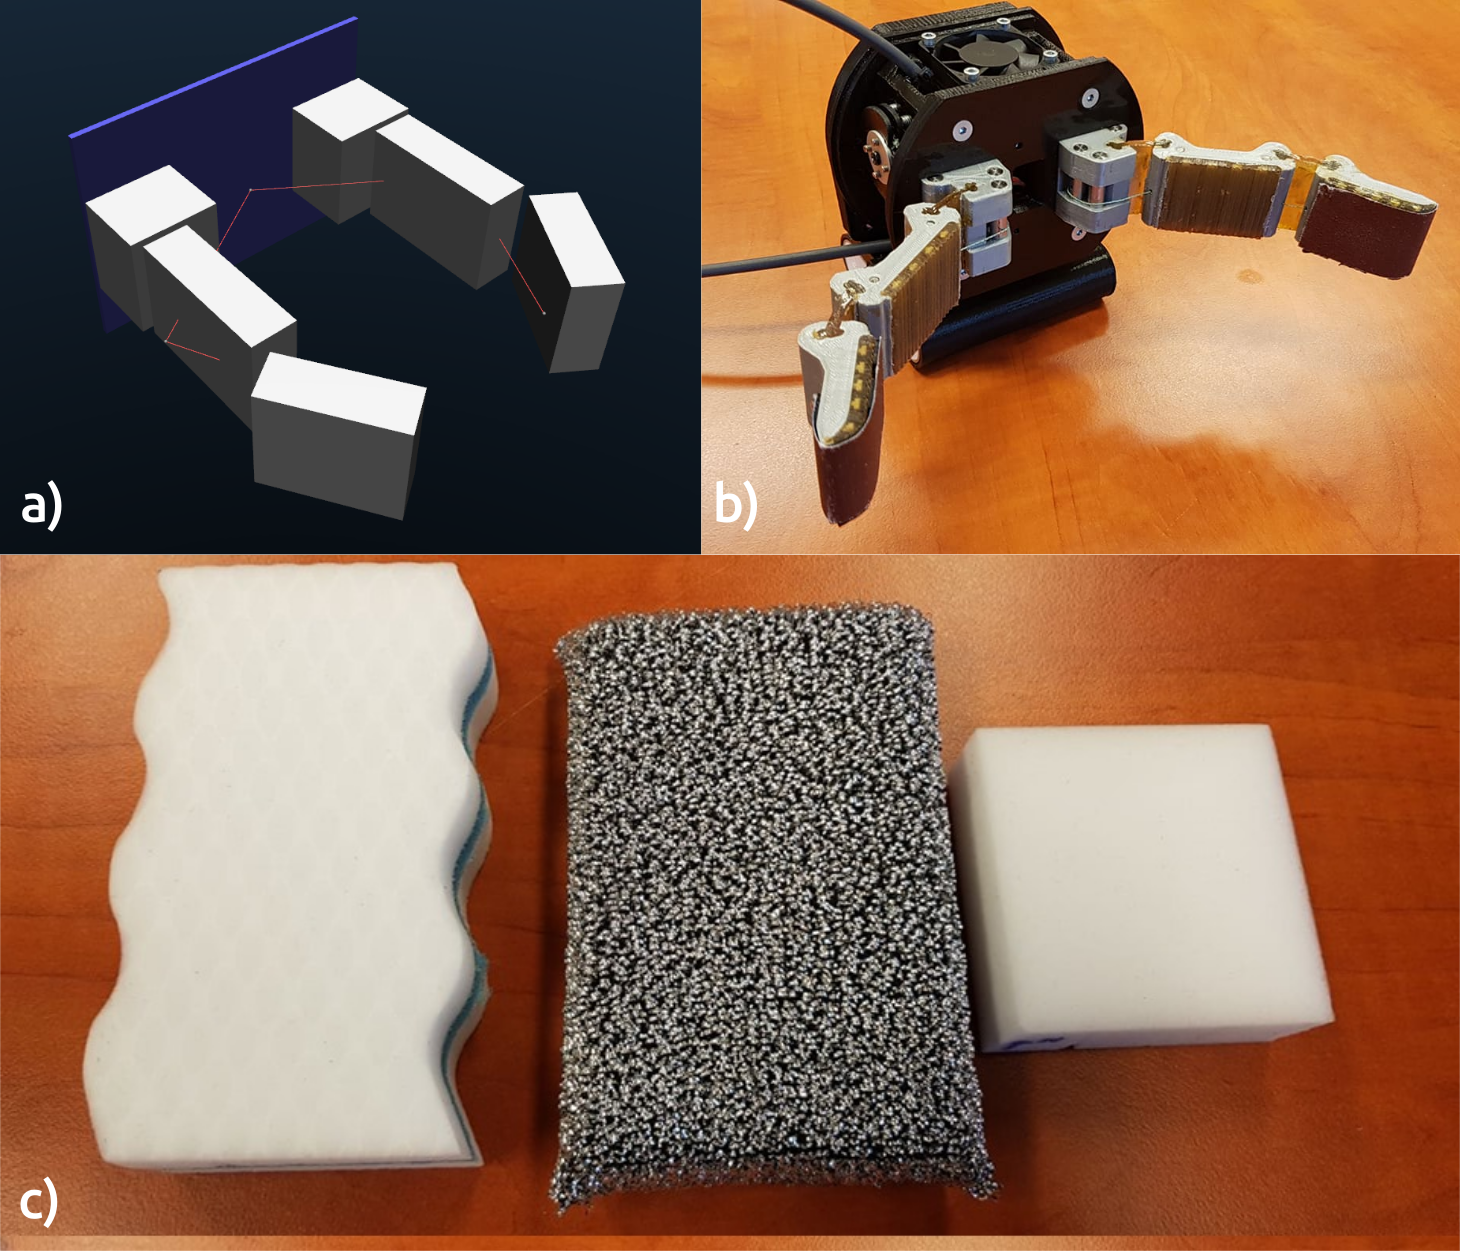
\includegraphics[width=0.7\textwidth]{images/gaining_sense_of_touch/real_experiments.png}
    \caption{The real-world scenario involved the 2-finger Yale OpenHand gripper~\cite{YaleOpenHand}. A sufficient number of training samples for the learning process had to be ensured. This gripper model was prepared in the MuJoCo simulator as depicted in \textit{a)}. In \textit{b)}, real fingers consist of three plastic blocks with flexible parts made of urethane. In~\textit{c)}, there are presented examples of sponges, exposing different stiffness, used in our real-world experiments.}
    \label{fig:real_experiment}
\end{figure}

\begin{table}[htbp!]
\centering
\caption{Stiffness coefficients were computed for five different objects using the presented procedure.}
\begin{tabular}{cc}
\hline
\textbf{Object} & \textbf{Stiffness {[}N/m{]}} \\ \hline
Wire sponge     & 909                  \\
Hard sponge     & 1020                  \\ 
Polish sponge   & 735                  \\ 
Soft sponge     & 380                  \\ 
Squash ball     & 1353                  \\ \hline
\end{tabular}
\label{tab:objects}
\end{table}

First, a coefficient $k$ was estimated for real-world objects in the $\calD_{real}$. The robot had a 3D-printed plastic bar mounted at the flange and pressed objects with the desired force using the Dynamic Force Control mode to obtain ground-truth values. In that mode, the manipulator accurately measured the displacement under specific forces. Thus, $k$ was computed according to the \Equation~\ref{eq:stiffness}, where $f_1$ and $f_2$ are forces in Z-axis while pressing an object with a tool and $\lvert d_1 - d_2\rvert$ is the relative distance that corresponds to the deformations under $f_1$ and $f_2$ respectively. The chosen objects express nonlinear behavior in their stiffness model (\eg the greater robot compresses the sponge, the less deformation it adds). However, objects did not reflect nonlinear effects in the specified range of exerted forces. Therefore, the estimated stiffness is considered homogeneous for the entire object. \Table~\ref{tab:objects} contains different stiffness coefficients $k \in \calK$ measured experimentally for each object.

\begin{equation}
    \label{eq:stiffness}
    k = \frac{\lvert f_1 - f_2 \rvert}{\lvert d_1 - d_2\rvert} \in \calK
\end{equation}

Afterward, the Yale OpenHand was used to perform the squeezing motion of each object and 500 \acrshort{imu} signals $m \in \calM_{IMU}$ registered during motions were collected. Each signal $m$ in $\calD_{real}$ consists of 12 sensor readings. Each of them was 200 time-steps long. In $\calD_{real}$,  each object is equally represented by 100 samples and split into two subsets -- 200 train and 300 test samples for the sim-to-real experiments. Both subsets in all the experiments remain unchanged. The following claim was made to address the physical interpretation of obtained parameters $k$ taking as input measurements $m$: The motion of gripper fingers registered while squeezing different objects would significantly vary, as shown in~\Figure\ref{fig:physical_interp}. One can observe that depending on the object's stiffness, the magnitude, and oscillations of both - angular velocity $\boldsymbol\rotvel$ and linear accelerations $\mathbf{\acc}$ were significantly different from each other, \ie in the range of values or an oscillation rate. Taking that phenomenon into account, this Chapter puts forward the thesis that it is possible to distinguish between different stiffness parameters in the space of \acrshort{imu} signals registered during the squeezing of these objects.

\begin{figure}[htbp!]
\centering
    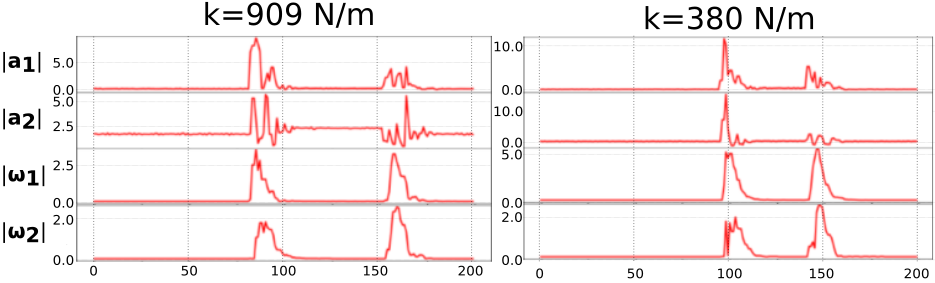
\includegraphics[width=0.95\textwidth]{images/gaining_sense_of_touch/physical_interpretation.png}
    \caption{Comparison between exemplary samples from the real-world dataset while squeezing objects with different stiffness values with a soft gripper. Values $|\boldsymbol\acc_{1}|$, $|\boldsymbol\acc_{2}|$, $|\boldsymbol\rotvel_{1}|$ and $\boldsymbol\rotvel_{2}|$ refer to magnitudes of accelerations and angular velocities registered by two \acrshort{imu}s and are expressed in $\frac{m}{s^2}$ and $\frac{rad}{s}$ respectively.}
    \label{fig:physical_interp}
\end{figure}

The number of samples, as well as distinct objects, remained limited. The root cause was the soft gripper's time-consuming data-gathering process and hardware limitations. In that situation, the number of different labels was insufficient to perform a successful regression without overfitting. In fact, with such a low diversity of accessible objects, a regression task would inevitably turn into a classification undesired in the stiffness estimation. A second dataset was based on the simulation to overcome that problem, where more training samples could be generated. Stiffness coefficients were adjusted to meet measured values.

\subsection{Simulated dataset}
\label{part:methods:materials:stiffness:simdataset}

Data-driven models frequently suffer from the limited ability to generalize to new domains outside their training dataset. However, the rising popularity of deep learning algorithms in the robotics community led to a significantly increased need for data. The state-of-the-art approach is to perform experiments in simulation and use the gathered data to feed neural networks. In a wide range of robotics applications, researchers can choose from many available physics simulators. In our case, the MuJoCo physics simulator was selected due to its efficient implementation regarding soft object modeling, which is troublesome in other simulators, \eg in the PyBullet~\cite{pybullet} or Gazebo~\cite{gazebo}. \Figure\ref{fig:scene_gripper_sim} presents the simulated soft-robotic gripper. Tendons connect fingers and are pulled by the actuator, which simulates the pneumatic cylinder. The simulation model basis on the 3-finger real gripper~\cite{MIT3fingerGripper}, but with one finger removed. As it is depicted in~\Figure\ref{fig:scene_gripper_sim}a, the $\calD_{sim}$ consists of samples when the gripper squeezed and released objects of three shapes - a ball, a box, and a cylinder, all with a variable $k$. For the elastic deformations simulation of the gripper, each geometrical block of each finger was connected to others by three hinges. In this setup, ranges of each joint in a roll, pitch, and yaw axes could be adjustable, as was depicted in \Figure\ref{fig:scene_gripper_sim}b. Finally, each behaves similarly to the elastic finger.

\begin{figure}[htbp!]
\centering
    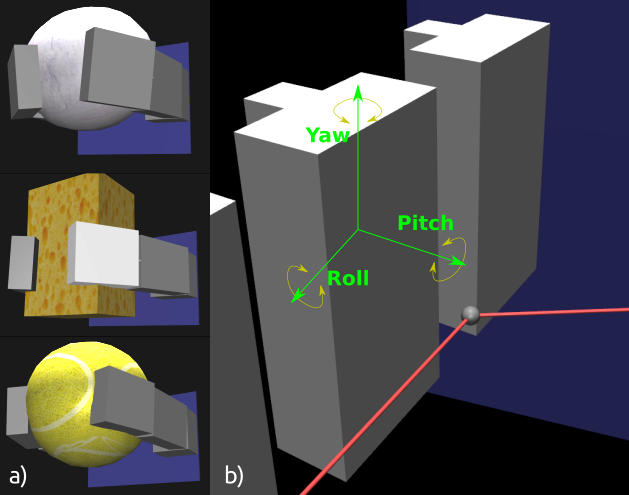
\includegraphics[width=0.7\textwidth]{images/gaining_sense_of_touch/scene_gripper_sim.png}
    \caption{Soft-robotic gripper in the MuJoCo environment: \textit{a)} the gripper squeezes and releases objects in three shapes - a ball, a box, and a cylinder, all with a variable stiffness parameter; \textit{b)} each geometrical block of each finger is connected to others by three hinges. In this setup, one can easily adjust the ranges of each joint in roll, pitch, and yaw axes.}
\label{fig:scene_gripper_sim}
\end{figure}

For clarity, a stiffness parameter $k$, in $\calD_{sim}$ was defined the same way as the MuJoCo simulator -- as the stiffness of a spring attached to a \acrshort{cog} of a geometrical block and its surface. The experimental section always assumes that the object is homogeneous.

The collection of data proceeded accordingly. Firstly, the object appears between fingers, and the actuators start to close the gripper and squeeze it. Then, in half a duration of a squeeze episode, the gripper opened up. While this process, an object was embraced by fingers that adapted to its shape. A stiffness coefficient $k$ was expressed in $\frac{N}{m}$ and varied among episodes to equally cover the range (from 300 to 1400$\frac{N}{m}$), which fits the real-world data range. Masses of gripper parts were adapted to meet real-world values. Similar to objects' mechanical impedance, their dampings, stiffness of all joints and springs in a system. Two \acrshort{imu}s were placed on a MuJoCo's element called \textit{site} and located in the 3/4 of the length of each finger on the outside surface. The first from two simulation datasets resembled the real-world data and consisted of 5000 training-validation samples from squeezing the box object. Its purpose was to enrich real-world data. The second simulation dataset consisted of three shapes: boxes, cylinders, and spheres. It counted 3999 training-validation samples, which gave 1333 samples per object. It served to verify whether any of the neural networks $f^{\prime}$ can avoid overfitting to any particular shape. Additionally, the model's generalization abilities were investigated using three test datasets -- 133 samples for each object.

\subsection{Recurrent neural network architecture}
\label{part:methods:materials:stiffness:models}

In Section~\ref{part:experiments:materials:stiffness} on the experimental evaluation, the main task of proposed neural networks was to approximate the stiffness estimation function $f$ from fixed-length sequences $m \in \calM_{IMU}$ of accelerations and angular velocities measured by \acrshort{imu}s. This research proposes to test three types of neural networks -- the \acrshort{cnn} $f^{\prime}_{conv}$ based entirely on 1D convolutional blocks, the \acrshort{cnn}-\acrshort{lstm} $f^{\prime}_{lstm}$ with forwarding \acrfull{lstm} units~\cite{LSTM}, and the \acrshort{cnn}-\acrshort{bilstm} $f^{\prime}_{bilstm}$ with \acrfull{bilstm} units~\cite{BiDirRNN}. In both recurrent models, the recurrent unit appears after the convolutional block. A \acrshort{fc} layer named the Regression Block is at each model's end. \Figure\ref{fig:nn_scheme} Presents the scheme of proposed neural network architectures used in the following work.

\begin{figure}[htbp!]
\centering
    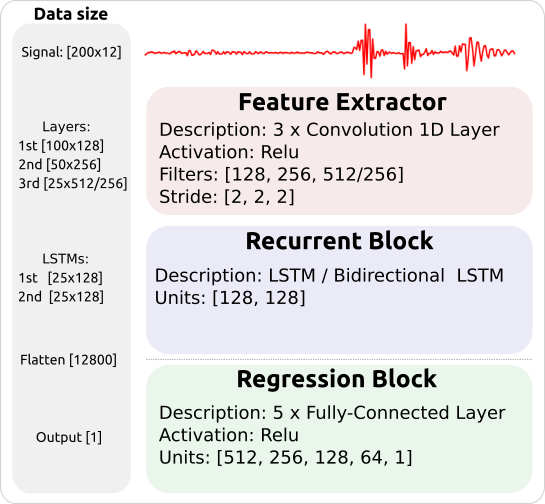
\includegraphics[width=0.7\textwidth]{images/gaining_sense_of_touch/overview.png}
    \caption{The Feature Extractor produces features using 1D convolutions. In the $f^{\prime}_{lstm}$ and the $f^{\prime}_{bilstm}$, the Recurrent Block process these features to find relevant connections for the stiffness estimation. Finally, the Regression Block outputs a stiffness coefficient $k \in \calK$.} 
\label{fig:nn_scheme}
\end{figure}

\paragraph{Feature Extractor} This module is responsible for extracting features from the raw signals while maintaining its output in the time domain. The input signal was a standardized sensor reading of 200 $m$ samples consisting of $2\times6$ measurements. Hence, data could be further processed recurrently or passed to the Regression Block directly. The Feature Extractor consisted of 3 consecutive 1D convolution layers with strides equal to 2. The number of filters in the layers of the \acrshort{cnn} was 128, 256, 512, while in the \acrshort{cnn}-\acrshort{lstm} and \acrshort{cnn}-\acrshort{bilstm} models, the last convolutional block was reduced to 256 filters and replaced by the recurrent block of the same size.

\paragraph{Recurrent Block} It processed high dimensional time series from the Feature Extractor in a recurrent manner using \acrshort{lstm} or \acrshort{bilstm} in $f^{\prime}_{lstm}$ and $f^{\prime}_{bilstm}$ respectively. A resulting, fixed-length vector representing an entire sensor reading maps the input from the time domain to the feature space. Each recurrent cell consists of 128 units, as it was shown in~\Figure\ref{fig:rnn}. In the \acrshort{cnn}-\acrshort{lstm}, both \acrshort{lstm} cells are organized in two sequential layers processing an input signal from the beginning to the end. Output features from that layer fed the Regression Block.

\begin{figure}[htbp!]
\centering
    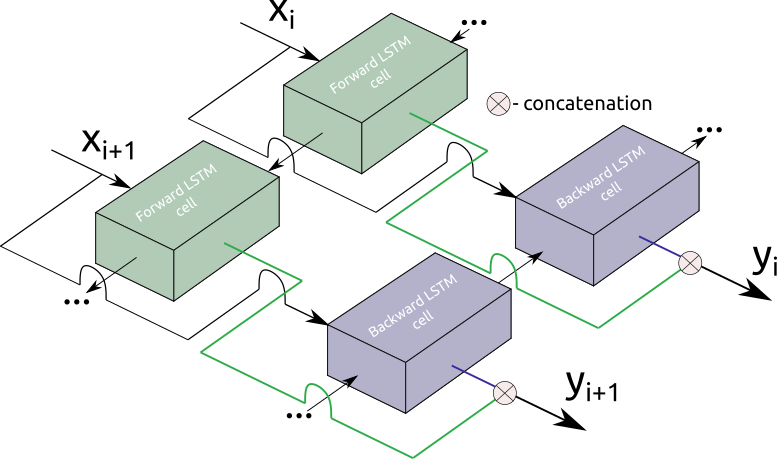
\includegraphics[width=0.7\textwidth]{images/gaining_sense_of_touch/rnn.png}
    \caption{The core idea behind the \acrshort{bilstm} used in the \acrshort{cnn}-\acrshort{bilstm} is as follows -- to prevent losing a context by the cell, process a sequence from the beginning to the end, do the same in the reversed direction, and concatenate both passes. Input $x_i$ refers to the $i$-th feature vector the convolutional block returns.} 
\label{fig:rnn}
\end{figure}

\paragraph{Regression Block} It was the last global module used in tested architectures. It was responsible for a final estimation of a stiffness coefficient $k$. Using a \acrshort{fc} layers is necessary because extracted features and time dependencies between them are critical ingredients in the regression process, but they are not the answer itself. Finally, it is necessary to transform obtained features into a stiffness coefficient $k$, made by the stacked \acrshort{fc} layers. The number of units in each layer remained unchanged for all tested architectures and was 512, 256, 128, 64, 1.

\subsection{Discussion on chosen methods}
\label{part:methods:materials:stiffness:discussion}

The proposed models for stiffness estimation based on time series of accelerations and angular velocities from the IMU mounted to the gripper consist of a Feature Extractor, Recurrent Block, and Regression Block. The first model uses only the Feature Extractor and the Regression Block, which is a pure \acrshort{cnn} based on 1D convolutions with \acrshort{fc} layers at the top. The second model adds an \acrshort{lstm} cell as a Recurrent Block to the pure \acrshort{cnn} model, and the third model utilizes a \acrshort{bilstm} as a Recurrent Block.

The pure \acrshort{cnn} model has the advantage of being relatively simple to implement and train, and it can capture the local features of the time series well. However, it may struggle with capturing the long-term dependencies between the data points, which can be important in stiffness estimation. The \acrshort{cnn}-\acrshort{lstm} model can capture both local and global features by using the \acrshort{lstm} as a Recurrent Block. It can handle long-term dependencies and is more suitable for time series data than the pure \acrshort{cnn}. However, it may be more complex to implement and computationally expensive. Finally, the bidirectional \acrshort{cnn}-\acrshort{bilstm} model has the added benefit of using a bidirectional \acrshort{lstm} that can capture information from both past and future time steps. This makes it suitable for modeling complex temporal dependencies and potentially results in even higher accuracy in stiffness estimation. However, it is the most complex model of the three and may require more computational resources to train and evaluate. 

\section{Unsupervised haptic recognition}
\label{part:methods:materials:dec}

\subsection{Problem formulation}
\label{part:methods:materials:dec:problem}

Let the $f_e \colon \calS \mapsto \calZ$ be the encoding function that inputs raw time signals from the multidimensional domain $\calS \colon \{s \in \Real^n\}$ (\eg 3-axis forces). Then transforms them to the latent space $\calZ$, and $f_d \colon \calZ \mapsto \calS$ be a decoding function that maps these features to the original domain again. Let the clustering problem be a grouping of $n$ points, such that ${s_i \in \calS}_{i=1}^{n}$ into $p$ clusters, where each cluster is associated with a centroid $u_j$, where $j = {1, 2, ..., p}$. Given the theoretical formulation above following could be introduced:

\begin{itemize}
    \item the baseline of learning-based algorithms for clustering unlabeled data using evaluation metrics presented in subsection~\ref{part:methods:materials:classification:metrics}. If the input data was a time signal, $f_{e}$ for baseline methods was a well-known dimensionality reduction method Truncated \acrfull{svd};
    
    \item the author's implementation\footnote{https://github.com/mbed92/haptic-unsupervised} that follows~\cite{DEC}. It uses a gradient descent, a mean-square error loss function $l_{MSE}$, and divergence loss $l_{KL}$ to cluster incoming data into a predefined number of bins. The presented method can work on raw signals without $f_d$ and $f_e$. However, optionally, we can also use the latent representation, which approximates the encoding-decoding function $\hat{x}_i = f_d(f_e(x_i))$ to represent signals in the latent space, and in that space, do the clustering. That method and baseline algorithms are described further in subsection~\ref{part:methods:materials:classification:methods}. The distance between raw signals or latent vectors in the $\calZ$ and centroids $u$ in the form of an auxiliary Student's t-distribution used to calculate the \acrfull{kl} divergence loss $l_{KL}$ that minimizes these distances during a training phase;
    
    \item the $\calD_{touch}$ dataset of pairs $d_{touch} \colon (s, c)$ consists of real-world 3D force readings gathered while touching different materials using a robotic manipulator associated with one of ten semantic classes. That dataset was created by the author of the following thesis together with other authors of~\cite{bednarek19}. It is worth noting that, in the following experiments, there was no train/validation/test split because in unsupervised learning, we do not have access to labels, so there was no clear definition of how that split would look like. Additionally, real-world datasets typically suffer from a limited number of samples due to time and hardware constraints, as was the case here. Therefore, the author of the following dissertation resigned from splitting the dataset and focused on analyzing the results from all available samples;
    
    \item the \acrfull{bigs2}~\cite{biotac2} dataset $\calD_{biotac}$ of pairs $d_{biotac} \colon [(s, c)]$ that consists of electrodes readings gathered at the same time from the BioTac sensors mounted on a hand-like gripper while grasping one of 51 classes of objects. That dataset is a follow-up work of~\cite{bigs} that extends the previously used \acrshort{bigs} dataset. Consistent with the Touching dataset, there was no train/validation/test split;

\end{itemize}

\subsection{Touching dataset}
\label{part:methods:materials:classification:dataset}

\Figure\ref{fig:robot_touching_closeup} presents the 3-axis optical force sensor OptoForce used to create the Touching dataset. This sensor has a diameter of 32 mm, weighs 30 g, and its shapes resemble a human fingertip. It can measure forces by utilizing optical principles. In the central part of the sensor, there is an infrared emitter with four receivers. The semi-spherical rubber internal surface is layered with a mirroring substance. Hence, reflections of infrared rays are highly dependent on the deformation of this hemisphere. Force measurements have three dimensions, and the sensor's precision reaches 6.25mN. The OptoForce sensor has a nominal force capacity of 100N on the Z-axis and 50N on the X and Y-axis, and it can be overloaded on each axis by 200\%. Again, we used the collaborative robot UR3 to gather dataset samples. It can estimate forces and measure torques in joints, enabling us to perform touching movements by pressing with a maximum force of 25N on the Z-axis of the robot's base coordinate system. The overall setup is shown in \Figure\ref{fig:robot_touching_overview}.

\begin{figure}[htbp!]
\begin{center}
    \begin{subfigure}{.5\textwidth}
        \centering
        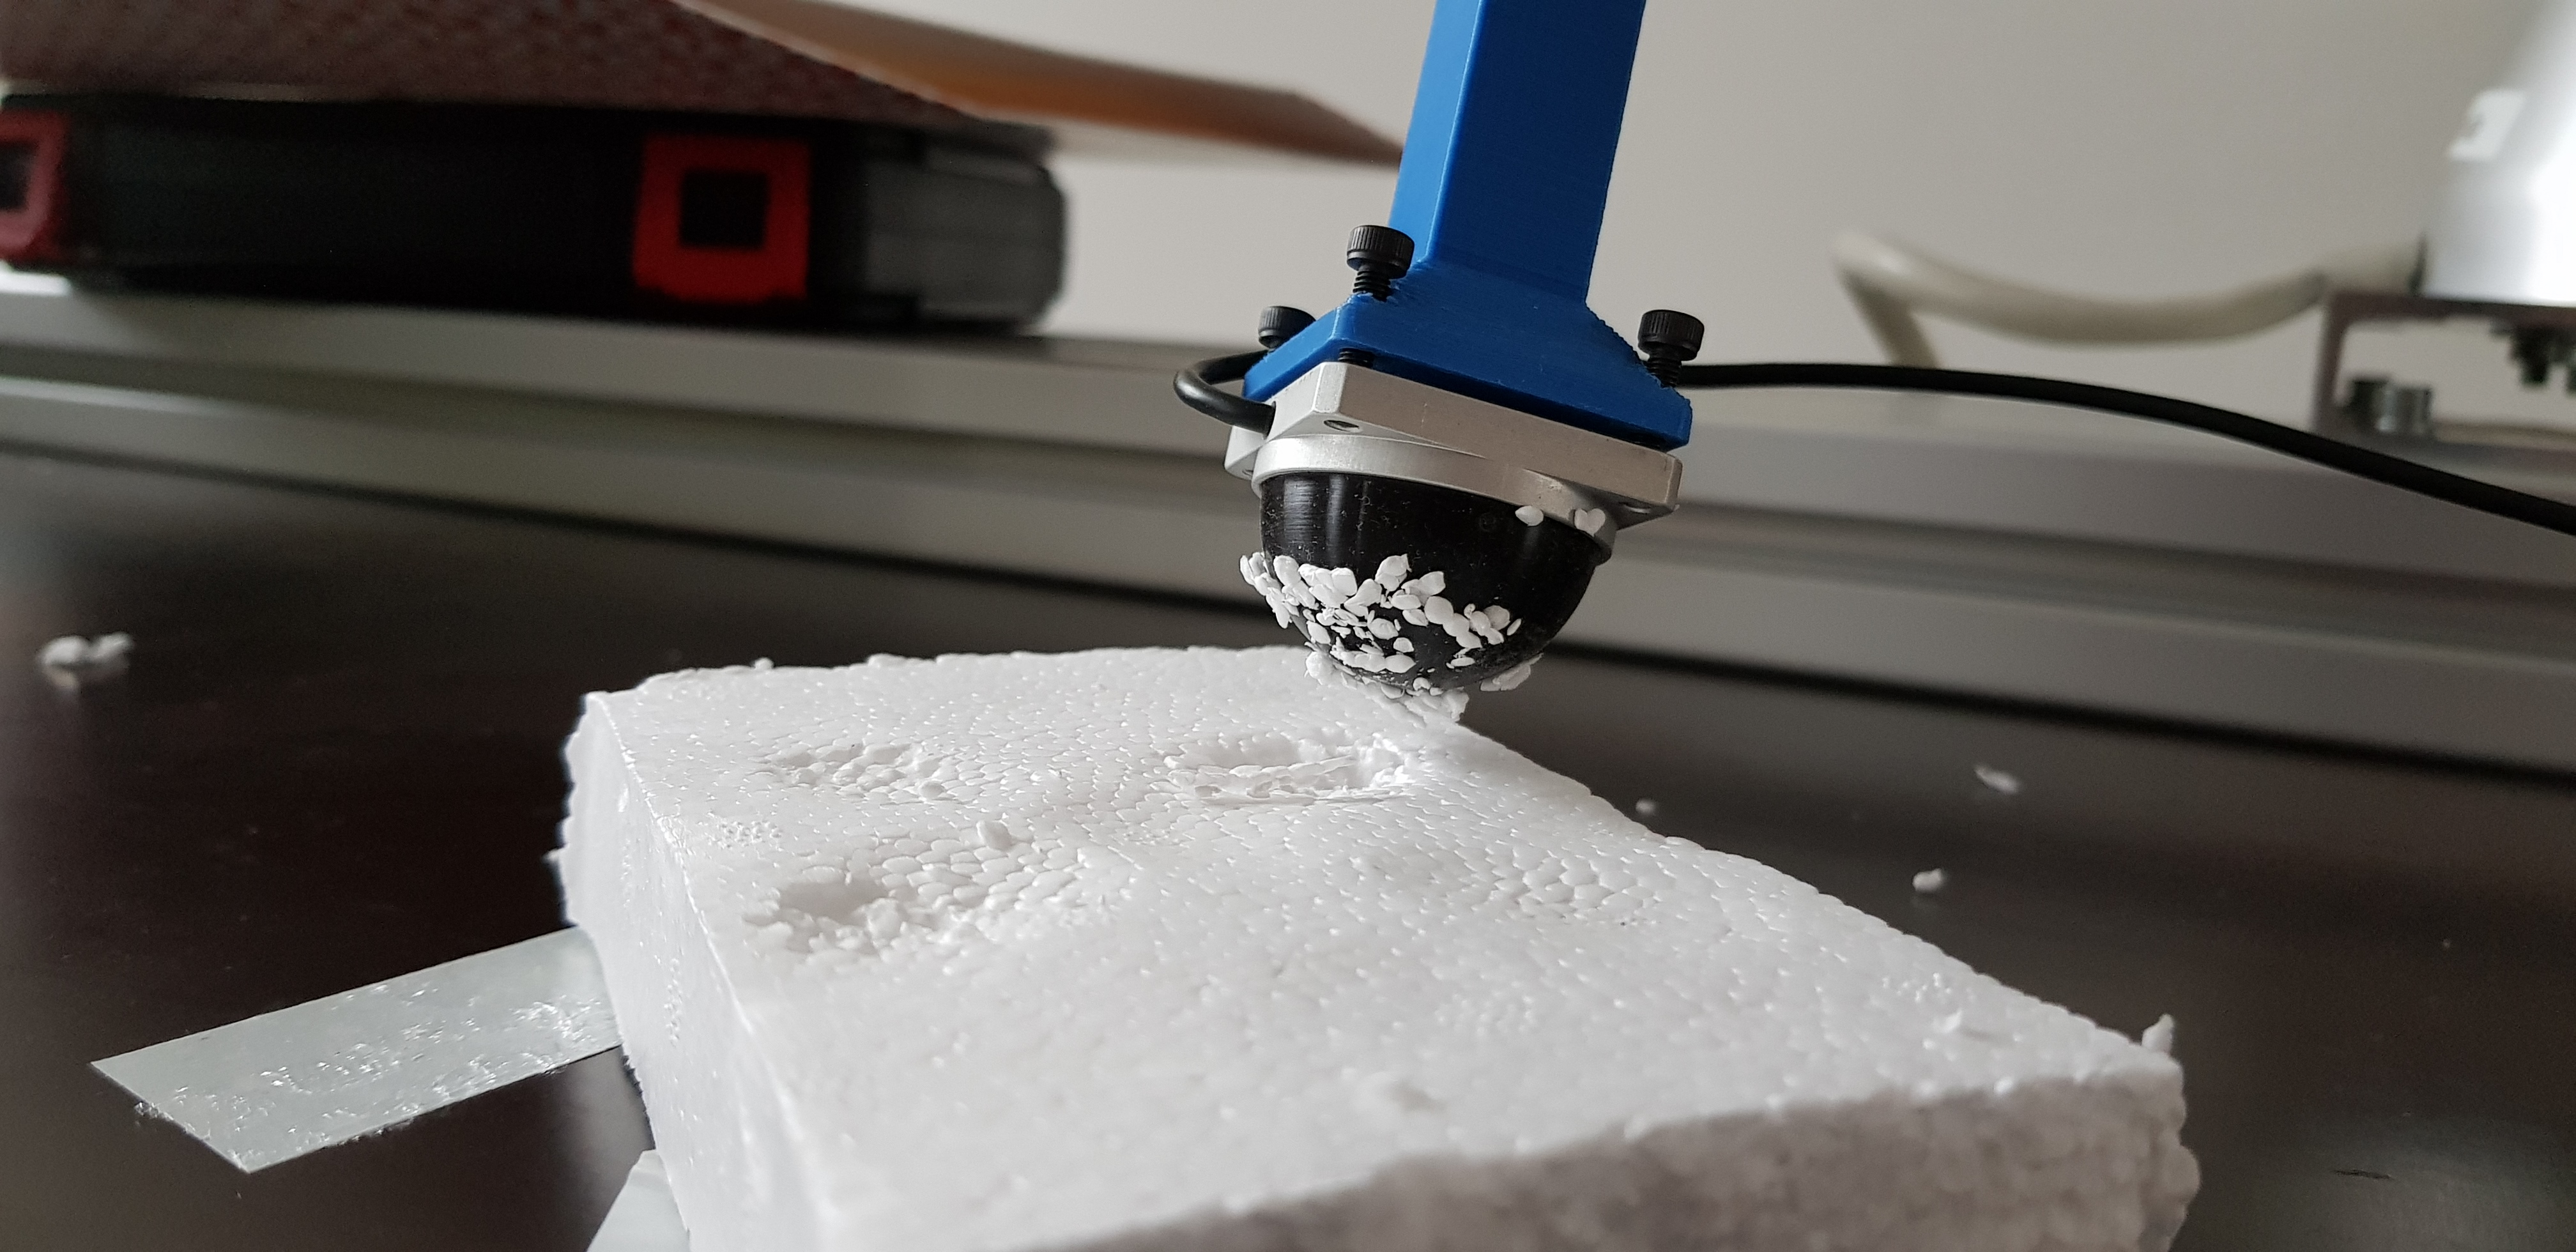
\includegraphics[width = 0.9 \columnwidth]{images/robotic_touch/robot_touching_closeup.jpg}
        \caption{Touching Styrofoam.}
        \label{fig:robot_touching_closeup}
    \end{subfigure}%
    \begin{subfigure}{.5\textwidth}
        \centering
        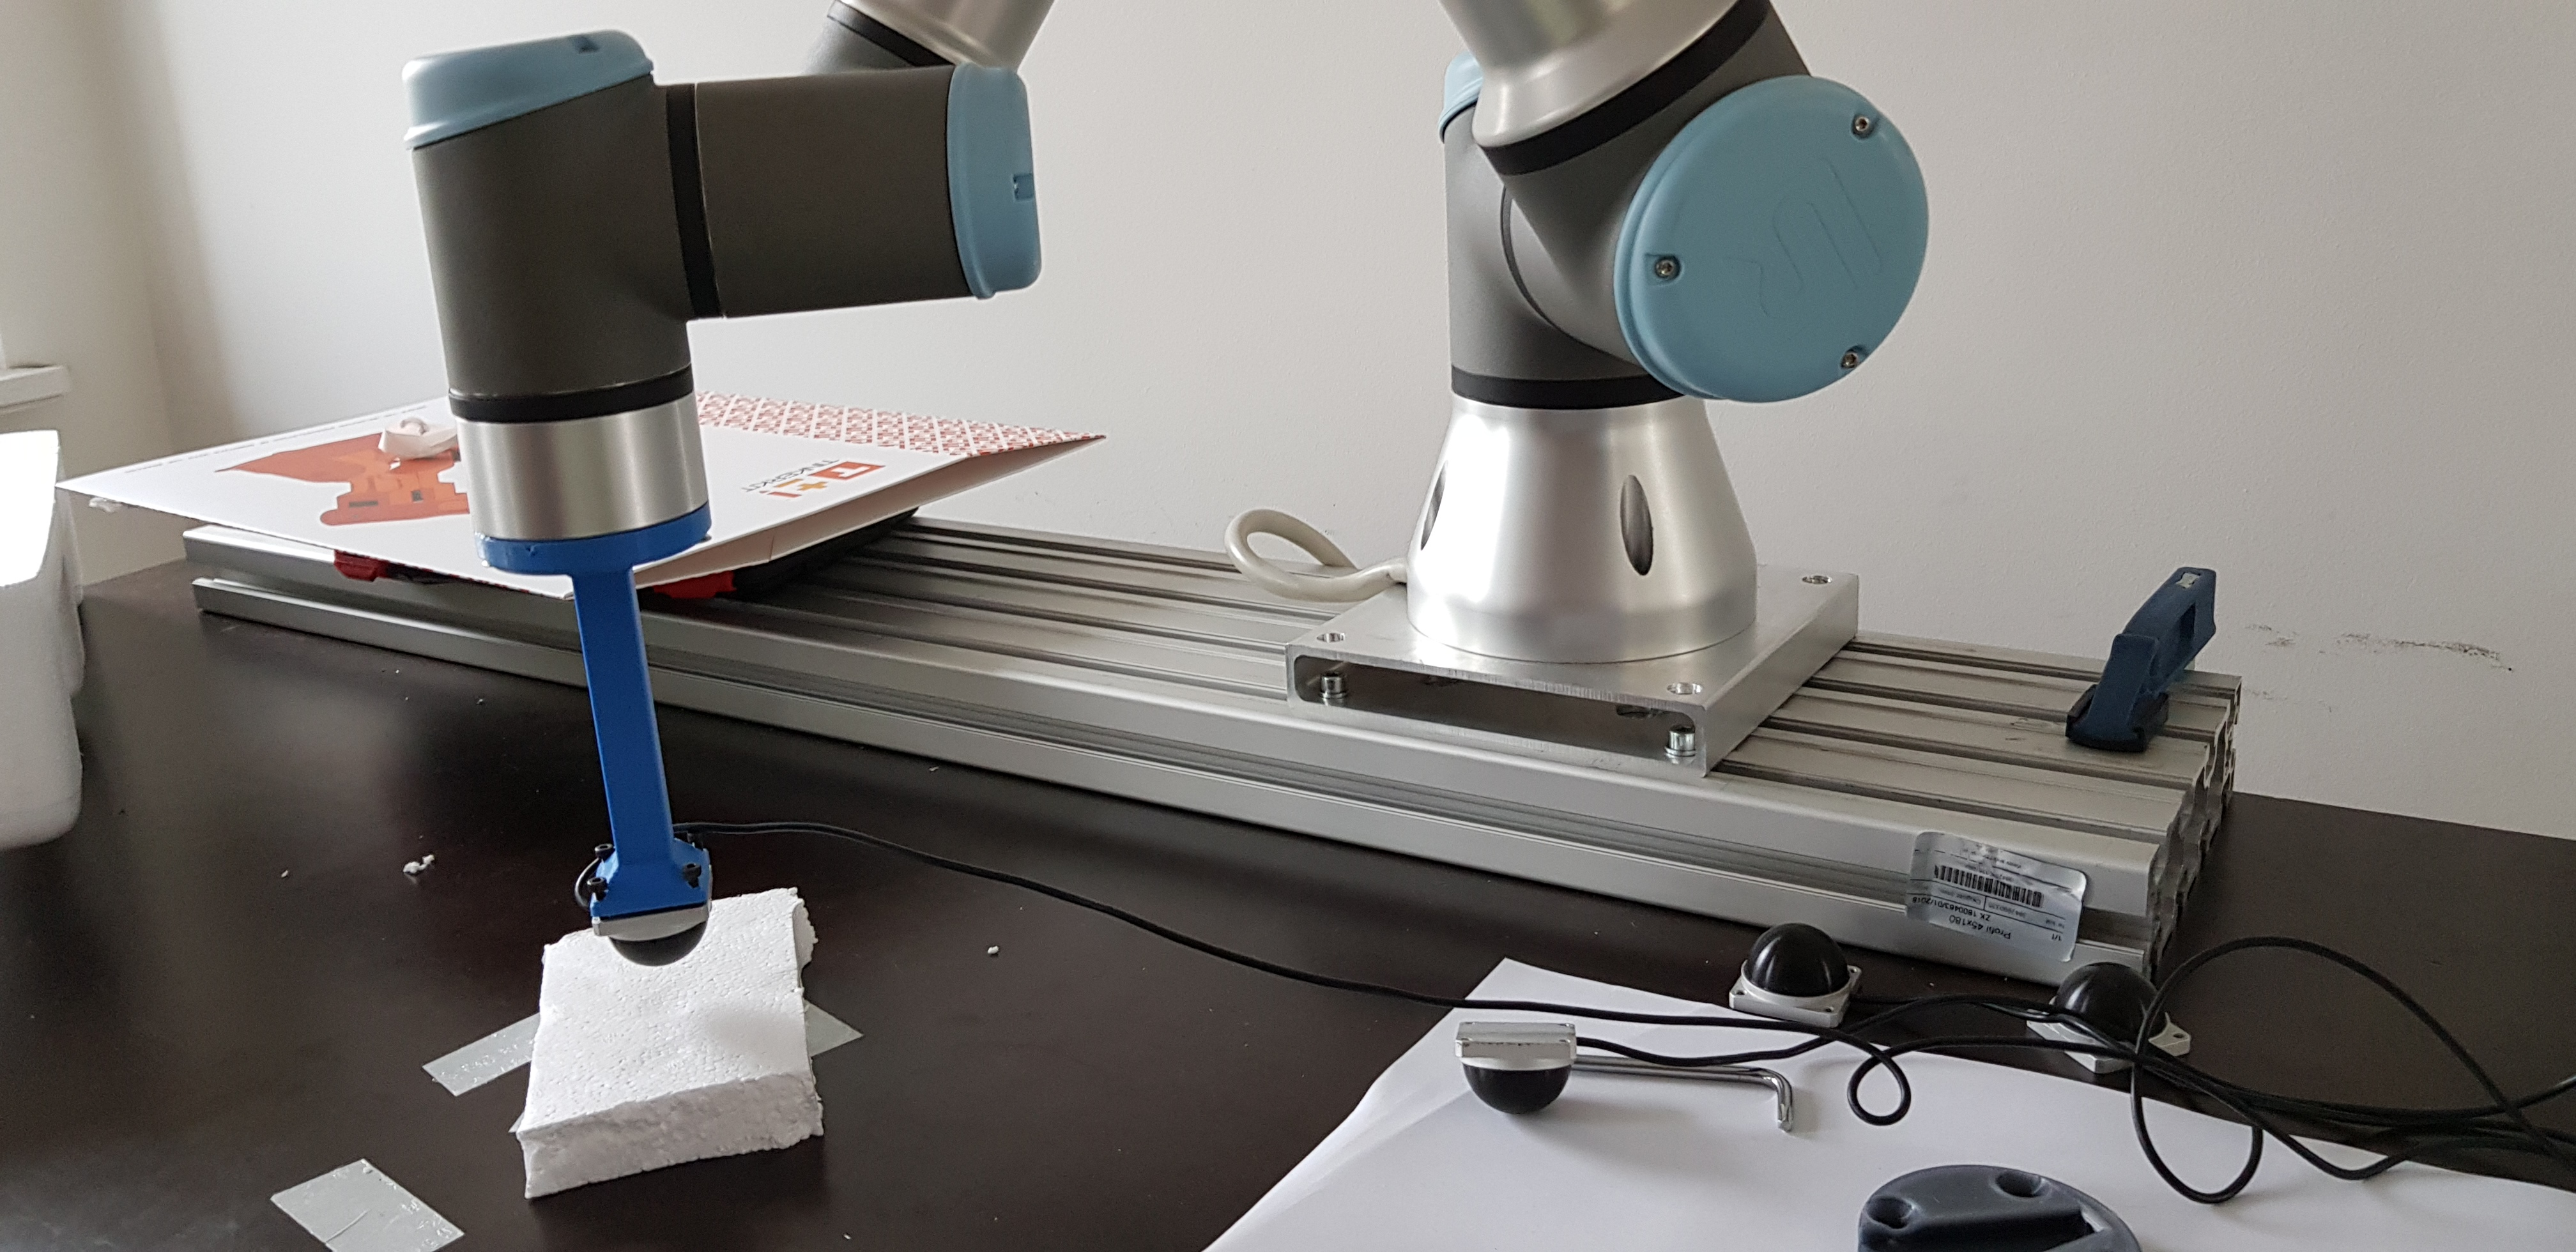
\includegraphics[width = 0.9 \columnwidth]{images/robotic_touch/robot_touching_overview.jpg}
        \caption{Overview of the setup.}
        \label{fig:robot_touching_overview}
    \end{subfigure}
\end{center}
\caption{The Figure presents robots and sensors used to create the touching datasets. The dataset focused on touching a variety of materials was created using a UR3 robot (\Figure\ref{fig:robot_touching_overview}) with an OptoForce sensor mounted on the top of the end-effector that is visible in \Figure\ref{fig:robot_touching_closeup}.}
\label{fig:dataset_gathering}
\end{figure}

The Touching dataset consists of 1293 labeled signals. Each sample consists of a 3-axis signal of forces recorded while touching the material with a length of 190 samples. The dataset includes ten classes of popular materials varying in thickness, stiffness, and texture. Items included are everyday objects, such as plane cardboard, corrugated cardboard, rubber, leather, linen bag, plastic plate, metal sheet, sponge, styrofoam, and a plastic bag. Sensors in experiments measure forces directly, allowing not only for the classification of materials but also to work on the regression, \ie estimation of physical parameters of the material. Using other sensors used for material classification from the contact, such as accelerometers~\cite{DALLAIRE2014422} or microphones~\cite{Kroemer11}, there is no possibility of estimating such parameters.

\subsection{\acrfull{bigs2}}
This dataset is an extended version of~\acrshort{bigs}~\cite{bigs} (used and described in other experiments of the following thesis regarding multi-modal fusion \ref{part:methods:fusion:multimodal:datasets}). The dataset follows the same structure as the original one and includes signals from it but adds 10 new classes, yielding possible benefits in any learning-based approach, especially unsupervised learning. That version consists of 5831 raw electrode readings recorded while grasping 51 different objects' categories. Each data sample is a measurement from three BioTac sensors mounted on a hand-like gripper. Three sensors on fingers are used to grasp objects, and each sensor returns a signal from 24 electrodes, giving 72 measurements per grasping episode. More information available in~\cite{biotac2} and the corresponding repository\footnote{\url{https://github.com/3dperceptionlab/biotacsp-stability-set-v2}}.

\subsection{Evaluation metrics}
\label{part:methods:materials:classification:metrics}

\paragraph{Clustering accuracy}
In the unsupervised setup, the accuracy might be obtained by solving a linear sum assignment problem~\cite{linear_sum_assignment} using a cost matrix $D$ of a bipartite graph. The $k \times k$  matrix $D$ includes assignments of each supervised class into unsupervised clusters. The metric achieves 100\% when all categories are separate clusters. In all algorithms to calculate the metric, the expected number of clusters was preset to the number of classes used at the training phase. However, it does not mean that the model will categorize data into the same number of clusters.

\paragraph{Mutual information}
The following metric~\cite{adjuster_mutual_info} shows the similarity between two clustering strategies in terms of the amount of surprise (or, in other words, uncertainty) in the results and mutual dependence between two random variables. It is typically used to evaluate the clustering quality or identify the most relevant features in a dataset. The non-normalized score ranges from zero to infinity, where higher values indicate more pure clusters. However, in the experiments, the normalized score was used. Similarly to clustering accuracy, it expects actual labels. Thus, it could be used with the desired number of clusters equal to the valid number of classes in the dataset.

\paragraph{Purity}
It shows to what degree each set contains one type (class) of samples -- how pure clusters are. Each group is assigned to the class most frequent in the cluster, and then the accuracy of this assignment is measured by counting the number of correctly assigned samples and dividing by the number of samples. Bad clustering has purity values close to 0. A perfect clustering has a purity of 1. High purity is easy to achieve when the number of clusters is significant - in particular, purity is 1 if each sample gets its cluster. Thus, we cannot use purity to trade off the clustering quality against the number of groups.

\subsection{Adapted methods}
\label{part:methods:materials:classification:methods}

\paragraph{Embedding clustering}

\acrfull{dec}~\cite{DEC} is a relatively new method that uses deep learning to learn feature representations of data, which are then used for clustering. This approach has several advantages over classical clustering algorithms from the Scikit-learn package. \acrshort{dec} can learn complex non-linear relationships in the data, whereas classical algorithms are limited to linear relationships. \acrshort{dec} allows deep embedding clustering, which produces more accurate and meaningful cluster assignments. Moreover, it is computationally efficient. It can handle large datasets and does not require extensive hyperparameter tuning, which can be time-consuming with classical algorithms. Overall, \acrshort{dec} is a powerful and efficient method for clustering data with many advantages over classical ones.

\paragraph{Ward}
The Ward algorithm is a hierarchical clustering method used to group objects based on their distance from one another. It works by iterative merging clusters to minimize the distance between the combined sets. This distance is typically measured using the Euclidean distance, the straight-line distance between two points. The algorithm continues to merge clusters until all objects are a single cluster. The result is a hierarchical tree or dendrogram that can be used to visualize the groupings of the entities.

\paragraph{Spectral}
It groups data points based on the eigenvectors and eigenvalues of a similarity matrix constructed based on the distance-based similarity between data points~\cite{SpectralClustering}. Eigenvectors and eigenvalues create a new feature space in which we look for clusters using other algorithms. The K-Means method was the final clustering strategy for these embeddings in the following experiments. However, it can be computationally expensive and sensitive to the choice of similarity measure. In the following experiments, the Spectral Clustering method is an improvement of the K-Means method with more sophisticated data preprocessing -- eigendecomposition reduces the number of features in the input data while preserving differences between data samples.

\paragraph{K-Means}
One of the most popular clustering algorithms used nowadays~\cite{tan2018introduction}. It scales well to large datasets and has been used across an extensive range of application areas in many fields. \textit{K} stands for the number of disjoint clusters in the data we expect. \textit{Means} refer to so-called centroids - the cluster centers we want to find. Finding sets is an iterative process of calculating distances from all data points to (initially random) centroids, classifying each sample based on the closest distance, and then recomputing centroids' positions by taking the mean of each created group. Generally, K-Means is a good starting point for clustering analysis because of its simplicity and speed (linear complexity). However, it is fragile to initial random choice of the centroids, and cluster shapes are considered elliptical, which is probably not valid in real-world data.

\paragraph{\acrfull{gmm}}
It is a probabilistic model that assumes that the data points follow a mixture of several multivariate normal distributions, each representing a cluster. The parameters of the \acrshort{gmm}, such as the mean, covariance, and mixing coefficients of the Gaussian distributions, are estimated from the data using the \acrfull{em} algorithm. The \acrshort{em} algorithm iteratively improves the estimates of the parameters until convergence, at which the data points belong to clusters based on the probabilities of each Gaussian distribution. The \acrshort{em} method is flexible and can handle non-spherical sets. Still, it can be sensitive to the initialization of the parameters.

\paragraph{\acrfull{birch}}
The method~\cite{birch} uses a hierarchical approach to identify clusters in large datasets. It starts by constructing an in-memory data structure called the Clustering Feature tree, which stores the feature vectors of the data points and summary statistics about the feature vectors. The Clustering Feature tree is constructed iteratively by inserting the feature vectors into the tree and merging similar nodes. Once we have the Clustering Feature tree, the clusters are identified by cutting the tree at a specific height, which determines the granularity of the groups. \acrshort{birch} is efficient and can handle large datasets, but it is sensitive to the choice of parameters, such as the maximum number of nodes in the Clustering Feature tree and the threshold for merging nodes.

\paragraph{Agglomerative}
A hierarchical clustering method works by splitting (top-down) or merging (bottom-up) data into groups and clustering by revealing a hierarchy presented originally in~\cite{sokal58}. The following experiments utilized the bottom-up approach. This method starts by treating each data point as a separate cluster, then iteratively merges the most similar clusters together based on the average distance between their points. It reveals the hierarchy in the data by a so-called dendrogram that can be cut at different heights to form a desired number of clusters.  Unlike other algorithms, it allows for the exploration of clusters at different levels of granularity. It is insensitive to the type of similarity measure used, but it brings a significant computational burden.

\subsection{Discussion on chosen methods}
\acrshort{dec} seems to be the best candidate for the specified task that has shown great potential in discovering meaningful structures in complex data such as images, text, and time series. Compared to other traditional clustering algorithms, \acrshort{dec} leverages the representation learning capabilities of deep neural networks to learn feature representations in an unsupervised manner automatically. Efficient representation learning lets the model identify underlying patterns and structures that may not be immediately apparent in the raw input data. Additionally, \acrshort{dec} is known to be more scalable and efficient than other methods, especially when dealing with high-dimensional data. Traditional methods rely on assumptions that could be unsuitable for such a complex task as unsupervised haptic recognition. \acrshort{gmm} assumes that the data follows the Gaussian distribution, which might not be accurate in real-world problems. Hierarchical algorithms like \acrshort{birch}, Ward, and Agglomerative clustering are sensitive to noise and outliers and may produce inconsistent results for datasets with high variability or irregularities. K-Means assumes that clusters are spherical and equally sized, which makes it inefficient in capturing complex and irregular shapes, as might be the case in haptic datasets. Finally, Spectral clustering may not be effective in identifying clusters with varying densities, as it relies on graph partitioning techniques that may need to handle such scenarios more effectively. \acrshort{dec} appears to overcome all the limitations of traditional methods. However, all methods tackle the clustering problem differently, and a thorough evaluation of the performance of all methods is necessary to ensure the best choice for the specific task. 

\chapter{Terrain recognition}
\label{part:methods:terrain}

\begin{notefromauthor}
    This chapter and the corresponding results in Part~\ref{part:experiments} incorporate material from the following publications.
    \begin{itemize}
        \item \ieee{2021} M. Bednarek, M. Łysakowski and J. Bednarek, M. R. Nowicki, K. Walas (2021) "Fast Haptic Terrain Classification for Legged Robots Using Transformer". In: European Conference on Mobile Robots (ECMR)
        \item \elsevier{2022} M. Bednarek, M. R. Nowicki, K. Walas (2022) "HAPTR2: Improved Haptic Transformer for Legged Robots' Terrain Classification". In: Robots and Autonomous Systems -- Selected papers from the 10th European Conference on Mobile Robots
    \end{itemize}
\end{notefromauthor}

\section{Introduction}
\label{part:methods:terrain:introduction}

The mobility of legged robots is a vital factor that gives them an advantage over wheeled platforms, which struggle to function in human-made domains with non-flat areas. Autonomously traversing kilometer-scale, natural environments demand excellent walking capabilities, \ie agility, robustness, and low-computational demand to avoid battery draining~\cite{AutoSpot}. They must fulfill a broad spectrum of mission-specific requests, including natural caves exploration, urban environments inspection (\eg sewers), or search and rescue tasks. One of the challenges of the real-world operation of legged robots is negotiating the unknown and unexplored terrain where the robot has to adapt its gait to the changing environmental circumstances. Planning and predicting the system's behavior in many scenarios is possible. However, there are cases when the robot has to react to unanticipated environmental measurements~\cite{aim}. In~\cite{DarioBellicoso2016}, authors presented such an adaptive behavior describing a robot's movement as a terrain function.

The following Chapter predominantly concentrates on the terrain classification with haptic contact, a well-researched topic with most solutions focusing on \acrshort{ft} signals from the sensors mounted on the feet~\cite{kolvenbach19,Ahmadi2021,bednarek2019icra,bednarek19}. These methods focus on obtaining the best results in accuracy measured on the registered dataset. However, the accuracy metric is only a part of the whole picture. A method should not achieve satisfactory classification only but also a short inference period. Moreover, computations should also be completed with limited processing resources as an autonomous walking robot has multiple nodes that must operate simultaneously to achieve desired outcomes in real-life challenges. Additionally, the following chapter argues that kinesthetic sensing, defined as sensing the position of a robot's limbs, leads to successful haptic perception. Typically, a sensor used to measure inertia in robotics is an \acrshort{imu} commonly mounted in a base of a walking machine. However, that placement is valid for kinesthesia because all haptic sensations, slopes, and terrain types must influence that sensor's readings.  
\begin{figure}[hbtp!]
    \begin{center}
        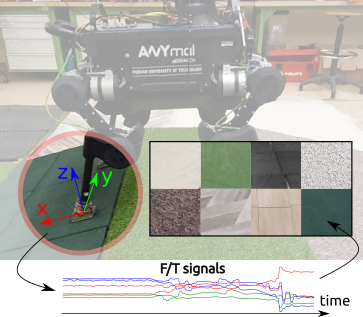
\includegraphics[width = 0.65 \columnwidth]{images/transformers/attentiongetter.png}
        \caption{\elsevier{2021} In the picture, the ANYmal robot collects haptic \acrshort{ft} measurements with its compliant feet when walking on diverse terrains. Terrain classification is paramount for gait adaptation to ensure stability. Moreover, there is a need to achieve a short inference period with resource-constrained processing units. Therefore, the transformer-based \acrshort{haptr} and \acrshort{haptr}2 methods were proposed.}
        \label{fig:anymal}
    \end{center}
\end{figure}

The following Chapter presents the deep learning model called \acrshort{haptr} with further extensions (\acrshort{haptr}2). Provided tests include a thorough evaluation of the \acrshort{haptr} model targeting previously omitted aspects like inference time and the method's robustness. This work contains a baseline in the results obtained with three adapted methods ranging from classical machine learning approaches to the \acrshort{cnn}. Moreover, the chapter provides results from other state-of-the-art solutions whenever possible and compares the accuracy on two publicly available datasets. Finally, an ablation study was employed to tackle the problem of the robustness of the proposed perception system. 

Therefore, the contribution presented in the following chapter comprises four items. Firstly, the work focuses primarily on transformer-based deep learning models for terrain classification -- \acrshort{haptr} and \acrshort{haptr}2. The lightweight implementation focused on short inference times and robustness against changes in input signals. Secondly, the research was conducted towards the \acrshort{mal} as a way to increase the robustness of terrain classification in real-world scenarios. Then, the experiments include a benchmark of terrain classification systems from the perspective of autonomy requirements. It includes the comparison of accuracy, inference time, and robustness against data degradation. Eventually, a transparent evaluation of the proposed and several adapted methods was included based on two publicly available terrain classification datasets to create a baseline for further works to compare and overcome the proposed solution.  All the code and datasets to reproduce the results are available online~\footnote{\url{https://github.com/mbed92/haptic_transformer}} publicly.

\section{Related work}
\label{part:methods:terrain:rw}

\subsection{Terrain recognition for legged robots}

In~\cite{Hoepflinger2010}, authors introduced one of the first contemporary approaches to terrain recognition for walking robots, where they tackled the problem of blindly assessing terrain properties using only currents from motors and contact forces of quadrupedal robot legs. Then, the AdaBoost~\cite{adaboost} algorithm processed extracted features from input signals, which revealed that a \acrfull{grf} is one of the essential properties describing a terrain under a moving leg. In~\cite{Wu2016}, authors proposed classifying terrain samples on tiny robots, where they directly measured a \acrshort{grf} from the designed miniature array of sensors. Direct measurements of the robot and ground substrate interaction were also described in~\cite{Li2017a}. A quadruped robot adjusted a \acrfull{cog} based on a terrain class to accommodate terrain properties changes. The step further in using terrain classification is to allow the robot to adapt its gate to changing traction conditions~\cite{Wu2020}. Predicting the risk of collapse of the structures negotiated by the legged machine~\cite{Tennakoon2020} is even further extension. Most of the research focuses on different types of hard materials, but there are also soft substrates in the dataset used in the following work. In~\cite{Bosworth2016}, the authors explicitly mentioned soft ground and provided the method of in situ measuring the terrain parameters. This work~\cite{Fahmi2021} and its further extension~\cite{Fahmi2020} presents a more analytical approach for the robots dealing with soft materials and gait adaptation. Terrain classification with other modalities like vision~\cite{Filitchkin2012} or acoustic sensors~\cite{Christie2016} is feasible yet less accurate than direct force measurements. For terrain classification, the fusion of three different modalities, vision, depth, and touch, was described in~\cite{Walas15a}.

Moreover, tactile data allowed for self-supervised visual terrain learning in~\cite{Wellhausen2019}. In~\cite{kolvenbach19}, authors analyzed tactile signals from impact motions of the quadrupedal robot's leg to classify different soil characteristics. In~\cite{bednarek19}, authors proposed a \acrshort{rnn} with convolutional blocks that achieved state-of-the-art results in the terrain recognition task. However, that method was able to work with fixed-length input data only. In~\cite{bednarek2019icra}, the masking mechanism for \acrshort{cnn}s was proposed to manage variable-length signals. In~\cite{Ahmadi2021}, authors also used raw and variable-length data recorded during walking sessions on different robots. Due to the semi-supervised machine learning approach, their terrain classification method achieved better performance than frequency-domain classifiers and required fewer annotations.

\subsection{Time series classification}

Time-series data mining has become an emerging field over the past decades due to the increased availability of temporal data~\cite{IsmailFawaz2019}. We can approach the problem by looking at the signal properties. Authors of~\cite{dtw_is_best} compared several similarity measures in the distance-based \acrfull{tsc}, showing that no individual distance measure is significantly better than the \acrfull{dtw}~\cite{DTW}. In the following experiments, a popular \acrfull{knn} classifier uses this distance measure to work on time-domain signals (\acrshort{knn}-\acrshort{dtw}), which the community considers a stable baseline in the field. However, authors of~\cite{dtw_is_best} also proved that using a heterogeneous \acrfull{ee} will outperform the \acrshort{dtw} even though any of the individual parts of EE were not achieving higher accuracy than \acrshort{dtw}. Authors of the \acrfull{cote} algorithm~\cite{cote} used such an ensemble of classifiers based on various feature spaces. The follow-up work -- \acrfull{hive} (\acrshort{hive}-\acrshort{cote})~\cite{hive-cote} leveraged the performance by the hierarchical voting system, which resulted in superior performance among other algorithms. The \acrshort{hive}-\acrshort{cote} is considered a state-of-the-art method for \acrshort{tsc}. Still, it exhibits a very high time-complexity due to many algorithms in an ensemble of classifiers. To illustrate that phenomenon, one of them -- the Shapelet Transform~\cite{shapelets} achieves the time complexity $O(n^{2}l^{4})$, which makes \acrshort{hive}-\acrshort{cote} impractical in many real-time scenarios~\cite{IsmailFawaz2019}. Authors of~\cite{BOSS} presented the \acrfull{boss} algorithm, which extracts words from input signals and learns to classify them in that space by measuring the frequency appearing of each word in a time series. An alternative method was presented in~\cite{ProximityForrest}, where the decision tree forest partitions the data under chosen distance measure. 

Recently, learning-based approaches started to play a significant role in the \acrshort{tsc}. In the range of state-of-the-art methods, the \acrshort{rnn}s with convolutional blocks, or \acrfull{cnn}s, play a prominent role. In~\cite{IsmailFawaz2020}, authors proposed the InceptionTime classifier based on the Inception-v4~\cite{inception} architecture that achieved cutting-edge scalability with decreased training time. A similar approach, called the \acrfull{rocket}, was proposed in~\cite{Dempster2020}. The authors showed that their model achieves state-of-the-art accuracy while maintaining a relatively short training time. It was possible by using multiple convolution kernels instead of stacking an ensemble of classifiers. In~\cite{bai2018empirical}, authors presented the \acrfull{tcn} as a convolutional alternative for \acrshort{rnn}s with a comprehensive comparison to the state-of-the-art recurrent models. 

Despite the undeniable success of transformers~\cite{transformers} in natural language processing~\cite{GPT3}, image recognition~\cite{dosovitskiy2020image} or object detection~\cite{DETR}, no prior works used transformers in the terrain classification in the real-world scenario with a walking robot.

\section{Proposed solution}
\label{part:methods:terrain:solution}

Mobile robots' popularity stems from their design, enabling them to interact with the environment in a plethora of outdoor and unpredictable scenarios~\cite{Miki2022}. Because of their versatility, resistance to environmental changes, and adaptive behavior, more and more companies consider them for commercial usage~\cite{Spot, Agility, Ghost, AnymalC}. Therefore, in many industrial applications, terrain recognition is a significant challenge. Walking robots can perceive their surroundings using various tactile-based or vision-based methods. However, vision-based methods exhibit limited applicability, as they are highly vulnerable to lighting conditions, fog, snow, dust, occlusions, low-texture surfaces, and other outcomes that might appear when a walking machine enters some hazardous area. One can observe that the focus of the robotics community turned mostly into tactile-based methods that utilize \acrshort{ft} sensors~\cite{kolvenbach19, Walas2016}, \acrshort{imu}~\cite{Ahmadi2021}, and proprioception~\cite{Walas15a, Cheng2019}.

The novel terrain classification method presented in this Chapter was primarily designed for fast and robust inference on a legged robot using raw sensory signals. The \acrshort{haptr} basis on the popular transformer architecture presented in~\cite{transformers} and~\cite{dosovitskiy2020image} formerly. The extensive experiments scope included an accuracy comparison on the \acrfull{putany}~\cite{KubaRNN} involving four different data-driven methods in multiple setups. Then, to verify our claims about the \acrshort{haptr}, there was added the section about cross-validation on another state-of-the-art \acrfull{qcat}~\cite{QCAT}, which presents the comparison against results presented in~\cite{Ahmadi2021}. Moreover, the work presents the novel \acrshort{mal} as a solution that increases the robustness of predictions against environmental impacts that might occur during a legged robot's operation. In all experiments, the \acrshort{haptr} achieved classification accuracy on the same level as the best models included in the comparison, having over 30×less learnable parameters and maintaining a short inference time. Finally, ablation studies on the \acrshort{mal} were included by deeply investigating its influence on the perception system's robustness.

\section{Terrain classification using Transformers}
\label{part:methods:terrain:haptr}

\subsection{Problem formulation}
\label{part:methods:terrain:haptr:problem}

Let the $f \colon \calS \mapsto \calC$ be the haptic classification function that assigns a discrete-valued class from the counter-domain $\calC$ to the raw, multidimensional signal sample from the set $\calS$. The set $\calS \colon \{s \in R^{n}\}$ consists of $n$-dimensional sensory signals from the available robot's equipment, such as \acrshort{ft} sensors, or the \acrshort{imu} mounted in its base. Typically, in the research software, the number $n$ is called the number of \textit{axes} of the input signal. The set $\calC = \{0, 1, 2, ..., c\}$ is integers, where $c$ is the total number of terrain classes expected in the dataset. Additionally, let the $f_{mod} \colon \calS \mapsto \calW$ be the modality weighting function that associates each multi-modal time series $s$ with a set of modality weights for each time step. The set $\calW \colon \{w \in \Real^{m \times t_{max}}\}$ includes floating-point numbers that correspond to the notion of \textit{importance} of input modalities, where $m$ is the total number of modalities, and $t_{max}$ is the time-length of an input signal. For the purposes of the dissertation, let's define \textit{modalities} as a set of axes associated with signal referring to the homogeneous physical value, \eg 3-axis \acrshort{ft} signals come from 2 different modalities. However, forces and torques might not be considered different modalities in the strictly physical sense, as they come from the same sensor for the sake of conciseness. The function $f_{mod}$ would associate to the \acrshort{ft} signal set of two weights for each time step, where weights at time $t$ are defined as $w_{t} = \{w_F, w_T\}$.

Given the problem formulation above, the following components of this work could be introduced:

\begin{itemize}
    \item an extensive comparison of classification methods in multiple experiments subsumed here under the common definition of $f^{\prime} \colon \calS \mapsto \calC$ for the sake of clarity, which approximate the function $f$ using deep neural networks or machine learning approaches;
    \item an attention module $f_{mod}$ in the form of a differentiable layer that increases the robustness of a function $f^{\prime}$ against input data deterioration;
\end{itemize}
\subsection{Terrain datasets}
\label{part:methods:terrain:haptr:dataset}

\paragraph{\acrfull{putany}} 

The following dataset is the set $\calS \colon \{\Real^{6}\}$ of 3-axis force and 3-axis torque data samples, where the ANYmal~\cite{anymal} robot was continuously walking on different real-world terrain samples with no additional exploratory moves. It had mounted \acrshort{ft} sensors on all feet. However, the dataset consists of samples representing signals from one foot only, so there was no information regarding which foot the signal was recorded from. \Figure\ref{fig:elevation} presents the map created with eight different terrain types. This dataset is the follow-up work of~\cite{bednarek2019icra}, but with the number of terrain classes $c = 8$ (previously six) and with several other improvements. Firstly, the robot had compliant, sensorized feet. Moreover, available terrains included also slopes to add samples at some inclination. Finally, all-terrain samples created a single walking area. The dataset is publicly available~\footnote{\url{https://drive.google.com/file/d/1QP-a1Y78LaKVN_mLt91b_10T_5YDyVD_/view}}.

\begin{figure}[htbp!]
    \begin{center}
        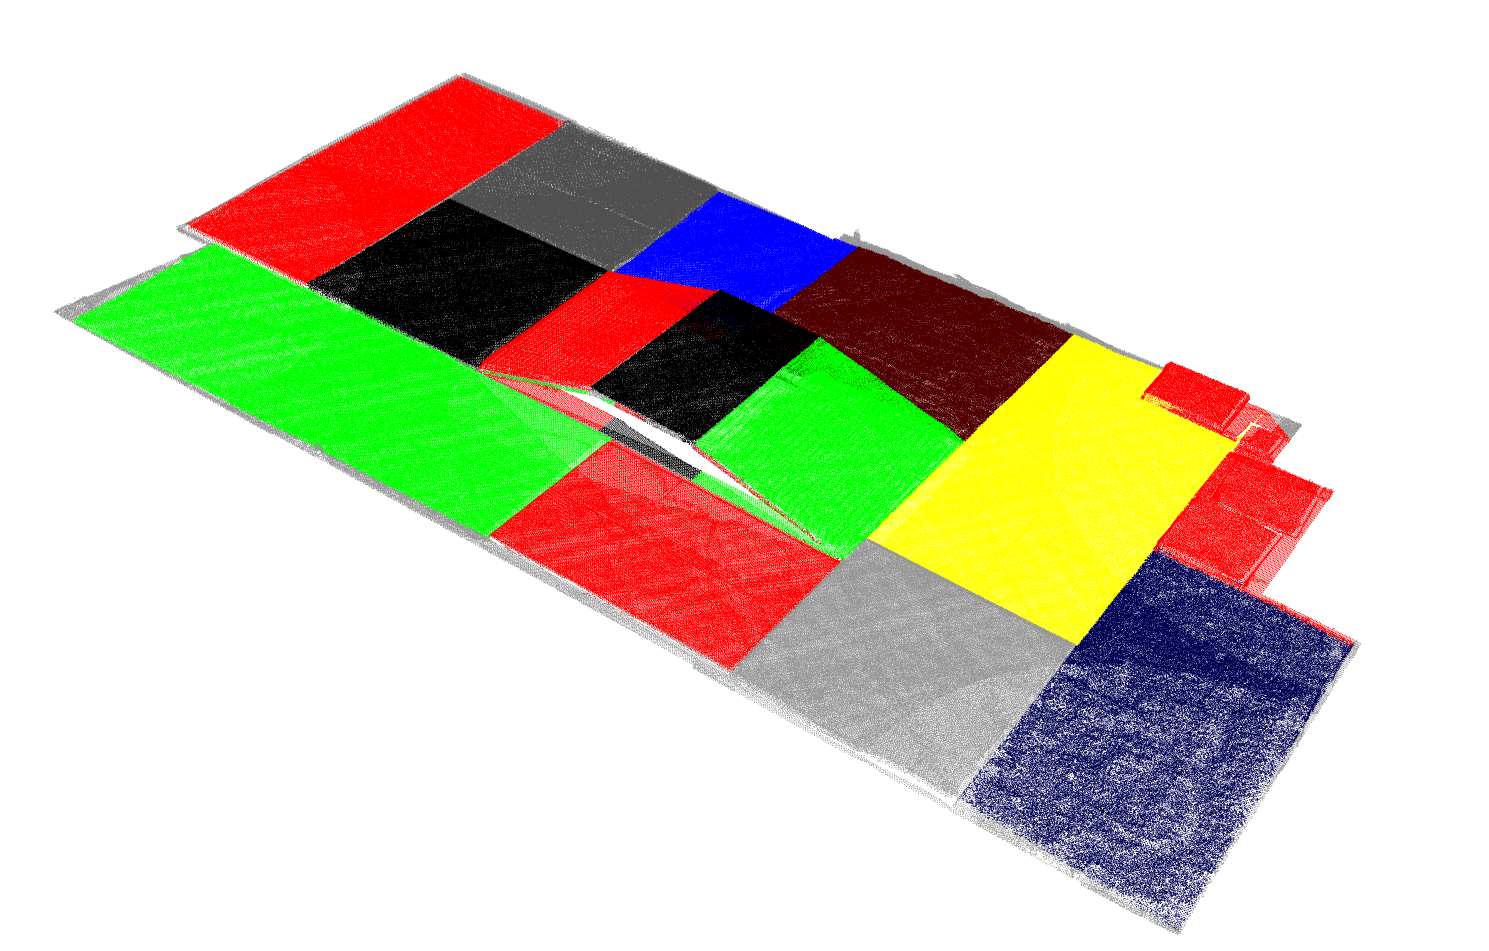
\includegraphics[width = 0.65 \columnwidth]{images/transformers/elevation_map_from_scanner.png}
        \caption{\elsevier{2021} The map with eight terrain classes and a slope was used to register the \acrshort{putany} dataset. The ground truth map for data labeling was registered with a 3D laser scanner (SURPHASER 100HSX), while the walking robot's pose was determined with the OptiTrack system. Colors correspond to different classes: red -- rubber, green -- carpet, blue -- \acrshort{pvc}, black -- artificial grass, yellow -- ceramic tiles, brown -- sand, dark blue -- rocks, grey -- foam.}
        \label{fig:elevation}
    \end{center}
\end{figure}

During the walking session, the ANYmal robot shown in \Figure\ref{fig:anymal} had sensorized, compliant feet~\cite{anyleg} that consist of flat contact surfaces with a range of motion $50^{\circ}$ for the pitch and $30^{\circ}$ for the roll axis. The robot traversed flat surfaces and a ramp requiring the feet to adapt to the terrain type and shape. \acrshort{ft} sensors placed inside the feet were custom-made and can sense up to 1000~N in the Z direction (along the robot's leg), 400~N in the ground surface, and up to 10~Nm of torque in each axis at a frequency 400~Hz. In the dataset \acrshort{ft}, signals were cropped to $t_{max} = 160$ registered during the instant of contact.

In the following chapter, eight different terrains were used (\Figure\ref{fig:terrains}): carpet, artificial grass, rubber, sand, foam, rocks, ceramic tiles, and \acrfull{pvc}. One can observe that the adaptive foot slopes differ depending on the terrain type, properties, and shape. The robot performed a statically stable gait with only one leg in a flight phase at a time. After a flight phase, all feet were on the ground. Then, a flight phase started all over again with a different leg.

\begin{figure*}[htbp!]
	\begin{center}
		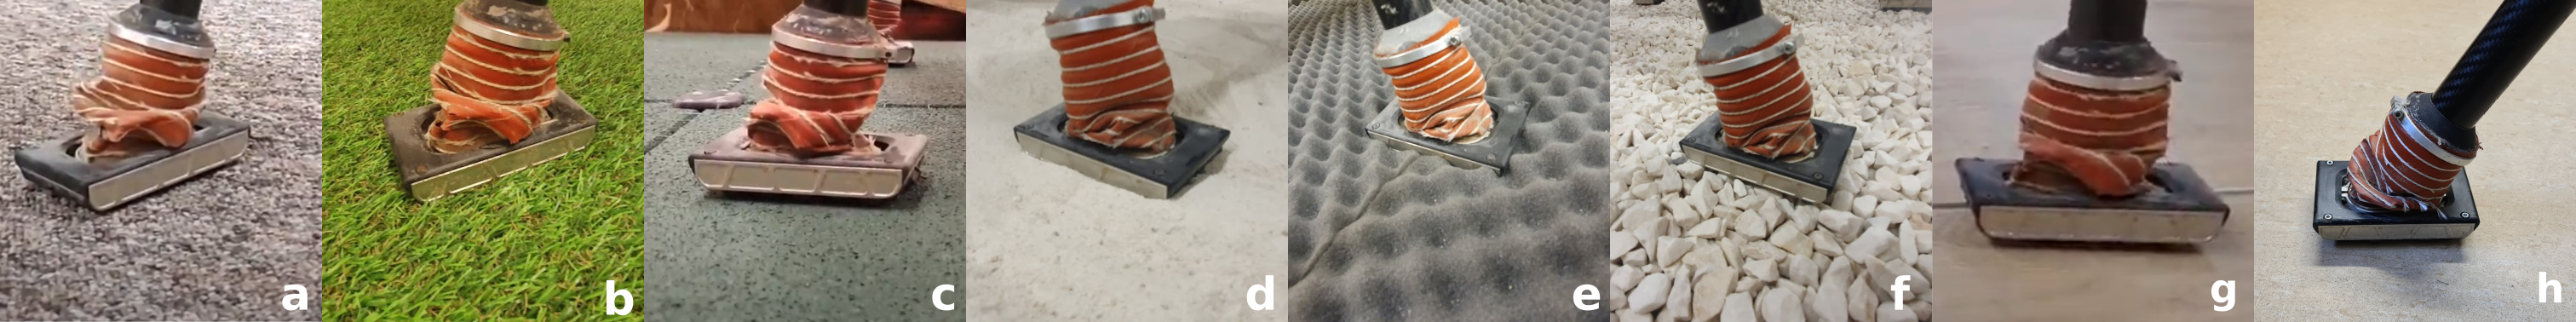
\includegraphics[width =  \textwidth]{images/transformers/terrains.png}
		\caption{\elsevier{2021} Terrain types included in the dataset: \textit{carpet} (a), \textit{artificial grass} (b), \textit{rubber} (c), \textit{sand} (d), \textit{foam} (e), \textit{rocks} (f), \textit{ceramic tiles} (g), \textit{\acrshort{pvc}} (h). Each terrain gave unique \acrshort{ft} feedback enabling the classification of these samples.}
		\label{fig:terrains}
	\end{center}
\end{figure*}

The dataset consists of recorded terrain samples divided into 3443 training, 1148 validation, and 1148 test subsets. Each signal contains 160 3-axis force and 3-axis torque measurements. The dataset comes from the continuous walking session, which is why it consists of an uneven number of samples registered for different classes (\Figure\ref{fig:hist} presents their distribution). In the dataset, there is no difference between samples for each foot. All samples have equal $t_{max}$.

\begin{figure}[htbp!]
    \begin{center}
        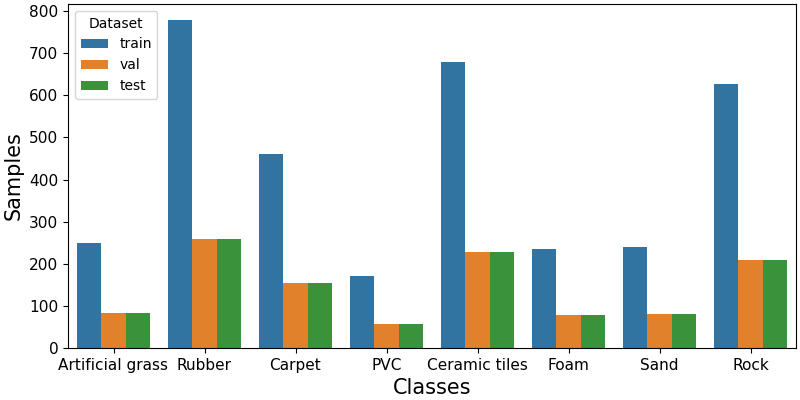
\includegraphics[width = \columnwidth]{images/transformers/histogram.png}
        \caption{\elsevier{2021} The distribution of terrain samples for the \acrshort{putany} dataset.}
        \label{fig:hist}
    \end{center}
\end{figure}

\paragraph{\acrfull{qcat}}

Another state-of-the-art dataset was employed to measure the performance of \acrshort{haptr} models -- the \acrshort{qcat} dataset. It consists of recordings from multiple walking sessions of the quadrupedal, self-configurable robot called DyRET~\cite{DyRET}. Raw signals come from the \acrshort{imu} mounted in its base and 3-axis forces from spherical sensors mounted at the tips of the robot's legs. 
DyRET~\cite{DyRET} is a four-legged robot with a dynamic morphology, designed to adapt the lengths of its limbs to different terrains. The kinematic chain of its leg was composed of two rotational joints intended for locomotion, and two, slow-changing prismatic joints for elongating and shortening the leg. It had the Xsens MTI-30 \acrshort{imu} mounted in its base consisting of a 3-axis gyroscope, a 3-axis accelerometer, and a 3-axis magnetometer. Each foot has the 3-axis force sensor Optoforce OMD-20-SH-80N.

The \acrshort{qcat} dataset consists of 2880 force and \acrshort{imu} samples -- 6 terrains $\times$ 10 trials $\times$ 6 speeds $\times$ 8 steps. Each force and \acrshort{imu} time series had $n = 22$ axes -- 4 $\times$ 3-axis force sensor and 2 $\times$ 3-axis angular velocities/linear accelerations, and 4-axis quaternion representing base's orientation. In the experimental section with the attention module, those axes created two modalities representing data from homogeneous classes of sensors  -- force and \acrshort{imu} separately. Each signal had $t_{max} = 662$. Similar to the \acrshort{putany} dataset, it does not differentiate feet or evaluate performance for each foot separately. The \acrshort{qcat} dataset is publicly available~\footnote{\url{https://data.csiro.au/collection/csiro:46885v2}}.

\subsection{Adapted methods included in the comparison}
\label{part:methods:terrain:haptr:models}

\paragraph{Convolutional neural network with recurrent modules (\acrshort{cnn}-\acrshort{rnn})}
In~\cite{bednarek2019icra}, authors tackled the problem of a terrain classification for the legged robots. In their experiments, they verified two deep learning models (\acrshort{rnn} and \acrshort{cnn}), a well-established \acrshort{svm}~\cite{SVM} as a baseline, and the \acrshort{fc} network working on \acrfull{fft} features extracted from raw signals. They compared all of the mentioned models on the fixed-length and variable-length time series. Both deep learning models and \acrshort{cnn} performed better than the traditional \acrshort{svm} method. However, this does not necessarily imply that they are faultless. Long sequences of \acrshort{ft} signals caused a well-known problem of gradient vanishing in the \acrshort{rnn}, resulting in significantly deteriorating classification accuracy. \acrshort{cnn} was free of this shortcoming, but using 1D convolutional layers forces working only on fixed-length input signals. Eventually, the feature-engineering solution based on \acrshort{cnn} required calculating the descriptors of input signals, thus, not achieving satisfactory accuracy. The most recent version of this model described in~\cite{KubaRNN} is the composition of all three components described before -- \acrshort{rnn}, \acrshort{cnn}, and the \acrshort{mlp} at the top. \acrshort{rnn} and \acrshort{cnn} components process variable-length data. When it comes to the \acrshort{rnn}, it is a natural consequence of the recurrence, but \acrshort{cnn} uses an additional masking mechanism. It pads variable-length input signals with zeros to match the fixed length. This model achieved the highest accuracy among all tested methods. 

\paragraph{Dynamic Time Warping K Nearest Neighbors (\acrshort{knn}-\acrshort{dtw})} The \acrshort{knn}-\acrshort{dtw}~\cite{dtw_is_best} was a baseline in the experimental section about the terrain classification. It is a well-established, distance-based classifier that uses the \acrshort{dtw} algorithm to measure the similarity between query signals (input time series) to the database of signals created during the training. While classifying, it determines the three closest matches (k=3) to the query signal by matching a training sample to the whole database. A training sample is then classified if the majority (at least 2) of matched sequences from the database represent the same terrain class. The experimental section includes results gathered using an efficient implementation of the \acrshort{knn}-\acrshort{dtw} in Python available in Sktime~\cite{Loning2019} library.

\paragraph{\acrfull{rocket}}
The authors of the \acrshort{rocket} algorithm proposed a method for the \acrshort{tsc} that works with a low computational burden while being invariant to the representation of the input features (\eg a shape or a frequency) because it uses a single, general mechanism -- a convolution. Firstly, some significant number of random convolutional kernels transform input time series into a feature space. The authors claim that these features -- in combination -- capture relevant information for the \acrshort{tsc}. Finally, any classifier might use them for training. However, the authors recommend linear classifiers (\eg a logistic or Ridge) because they can utilize a small fraction of information from all input features. Unlike artificial neural networks, kernels' weights are not learnable but randomized. Hence, the computational cost of training is low. The initial design was to work primarily with univariate signals. In the experimental section, each axis of \acrshort{ft} signal was transformed separately to a feature space using 10000 random kernels. Once in a feature space, different information channels were concatenated to form one feature sequence passed to the final classifier.

\paragraph{\acrfull{tcn}}
In~\cite{bai2018empirical} authors proposed a general, convolutional-based framework called the Temporal Convolutional Network for time series processing. It fits the requirements established in this work and handles longer sequences than recurrent neural networks. The \acrshort{tcn} consists of multiple 1D fully-convolutional layers, where all subsequent hidden layers are in the same length as previous ones. It keeps the output of the \acrshort{tcn} the same length as the input. The \textit{casual convolution} is a mechanism added to keep the past time samples away from the current ones, so there is no leakage from the future into the past. The more time steps are in the input signal, the more complexity it adds to the \acrshort{tcn}. To overcome this shortcoming, the authors proposed to use dilated convolutions with the exponential receptive field in the consecutive layers. This procedure allows handling significantly longer sequences while achieving a relatively low computational burden. The \acrshort{tcn} does not contain any form of memory or recurrence while providing state-of-the-art results. The original \acrshort{tcn} returns a features sequence, which does not apply to the task of terrain classification. Therefore, the adapted model includes the \acrfull{mlp} layer at the top to predict terrain classes. In the experimental section there were evaluated several configurations of the \acrshort{tcn} that differ when it comes to the number of convolution levels (LE), hidden units per each level (HI), and the number of hidden neurons in the (\acrshort{mlp}):

\begin{itemize}
    \itemsep0pt
    \item \textit{Light} - LE=4, HI=8, \acrshort{mlp}=128,
    \item \textit{Base} - LE=8, HI=16, \acrshort{mlp}=256,
    \item \textit{Large} - LE=16, HI=25, \acrshort{mlp}=256.
\end{itemize}

The authors of~\cite{bai2018empirical} shared the implementation of their \acrshort{tcn}, which was a basis for the experimental verification in the following work.
\subsection{Contributed methods based on transformers}
\label{part:methods:terrain:haptr:contributed}

\begin{notefromauthor}
    The following section presents two methods in chronological order, as they appeared in the publications of the author of this thesis. They work under the same principles. However, the second one was the follow-up work that included an improved version of the \acrshort{haptr} with the \acrshort{mal}.
\end{notefromauthor}


\paragraph{Haptic Transformer \acrshort{haptr}}

The most recent peak in popularity of transformers, specifically their application to computer vision problems~\cite{DETR}, was a foundation under consideration of this approach for terrain classification. No previous methods utilized transformer architecture to process multi-modal, raw sensory feedback to classify terrains. However, when writing this dissertation, it became apparent that other research groups were at the same time working on the same subject but in different research domains. The time series transformer appeared, \eg in~\cite{TST} -- the submission of this article took place one month after the author's initial \acrshort{haptr} article~\cite{ecmr21}, which indicates the high priority in the research community of the issue addressed. The \acrshort{haptr}~\cite{ecmr21} comprises the first proposition to tackle the problem using such an architecture. It uses a self-attention mechanism instead of convolutions to classify the terrain. As the authors of~\cite{park2022how} point out, the usage of multi-head attention modules improves the accuracy and generalization ability of the method by turning the training to domain-specific knowledge instead of data-specific (as is the case using convolutions), which would be beneficial in the robotic application. Similar to Vision Transformer (ViT) used in~\cite{dosovitskiy2020image}, the \acrshort{haptr} uses a learnable linear projection layer to map a signal $s\in\Real^{6}$ (\eg a 3-axis force and 3-axis torque) into a sequence of the same length $t_{max}$ in feature space of 16 axes. In the following work, samples of that sequence are called patches. Then, positional encoding (PE) is added to every patch to retain position information and passed to the Transformer Encoder Layer. Eventually, every vector is reduced in dimensionality before the final classification with the \acrshort{mlp}. The implementation of the \acrshort{haptr} is based primarily on PyTorch modules, especially TransformerEncoder and TransformerEncoderLayer.

For the \acrshort{haptr}, there were evaluated variants with a different number of encoder's layers (L) and attention heads (H). Models are referred as: 
\begin{itemize}
    \itemsep0pt
    \item \textit{Light} - L=2, H=4,
    \item \textit{Base} - L=4, H=8,
    \item \textit{Large}  - L=8, H=8.
\end{itemize}

\paragraph{Improved Haptic Transformer with the \acrshort{mal}}

The \acrshort{haptr} is the first attempt to tackle the problem of terrain classification using a transformer-based neural network. With a piece of domain knowledge about the problem itself, the \acrshort{haptr} evolved to an improved version called the \acrshort{haptr}2 as presented in \Figure\ref{fig:haptr}.

\begin{figure}[htbp!]
    \begin{center}
        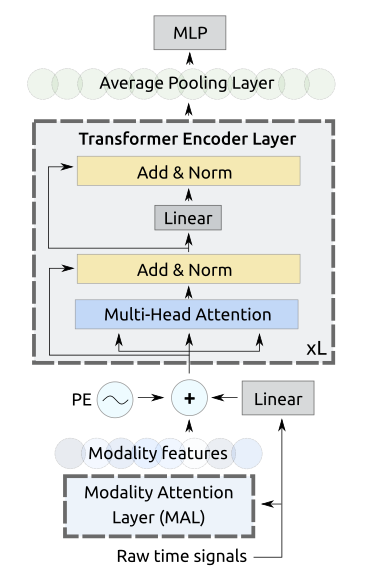
\includegraphics[width = 0.65\columnwidth]{images/transformers/models_v4.png}
        \caption{\elsevier{2022} Improved \acrshort{haptr} is the follow-up model based on~\cite{ecmr21} with \acrshort{mal}.}
        \label{fig:haptr}
    \end{center}
\end{figure}

The main novelty of the presented method is the \acrshort{mal}, which basis on the Multi-Head Attention mechanism introduced in the~\cite{transformers}. In~\cite{park2022how}, the authors show that the composition of the attention mechanism with convolutional layers is complementary and generally beneficial. The former behaves like a low-pass filter due to the weighting mechanism presented in the \Equation~\ref{eq:attention}, which flattens the feature maps. On the other hand, the convolutions are prone to capture high-frequency features and focus on data-specific knowledge (\eg spikes, slopes, mean and variance changes). This phenomenon suggests that using the multi-head attention mechanism would improve the robustness of the robotic system, which might undergo a plethora of data-degradation scenarios in the real world. The \acrshort{mal} implements the $f_{mod} \colon \calS \mapsto \calW$ function and assigns importance weights $w$ to the input modalities at each time step $t$. Firstly, input time series $s$ is split according to its modalities (\ie 3-axis force and 3-axis torque signals measured at the robot feet are separate modalities) and passed to 1D convolutional layers, which creates flattened representations of the multi-axes, modality signal representations of the same length $t_{max}$ as inputs. Learnable linear layers process and shape each modality representation to so-called queries (Q), keys (K), and values (V) for the dot product attention layer. There are as many queries as input samples. Then, each sample is weighted between existing modalities and scaled by the factor of ($1/\sqrt{d_k}$), where $d_k$ is the dimensionality of multiplied queries and keys. Therefore, the \Equation\ref{eq:attention} describes activation of the \acrshort{mal} layer:

\begin{equation}
    \label{eq:attention}
    Attention(Q, K, V) = softmax(\frac{QK^{T}}{\sqrt{d_k}})V.
\end{equation}

The keys are formed of a matrix with size $d_k \times d_k$. Rows represent a $d-th$ modality with $d=1, 2, ..., d_k$. Therefore, the closer the query is to the corresponding key, the higher weight is associated with that modality. \acrshort{mal} can work with any number of user-defined modalities, but in the scenario with forces and torques, they are two separate modalities. The $d_k$ is equal to 2, and keys are composed of the $2 \times 2$ matrix. Finally, a softmax is applied on the scaled dot-product to obtain a probability distribution. \Figure~\ref{fig:modatt_layer} presents the information flow of \acrshort{mal}. Typically in transformer models, the self-attention layer delivers weights between all time steps, e.g., in Natural Language Processing, to reveal the contextual associations between the first and other words in the sentence. Nevertheless, in the following work, the attention layer discovers weights between time steps and entire modalities rather than between all pairs of time steps in the input signal.

\begin{figure}[htbp!]
    \begin{center}
        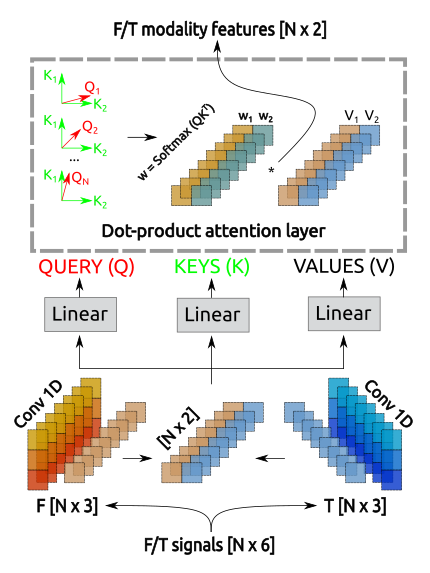
\includegraphics[width = 0.75\columnwidth]{images/transformers/modality_attention.png}
        \caption{\elsevier{2022} The visual explanation of the \acrshort{mal} used in the experiments. It was used to increase the robustness of the \acrshort{haptr} model.}
        \label{fig:modatt_layer}
    \end{center}
\end{figure}

Apart from the \acrshort{mal}, a complete list of changes introduced in \acrshort{haptr}2 in comparison to the initial version includes:
\begin{itemize}
    \item used an improved learning rate scheduling~\cite{loshchilov2017sgdr},
    \item an output from the \acrshort{mal} was concatenated with original input signals by channels axis,
    \item an average pooling layer replaced a mean operation before an \acrshort{mlp} classification layer,
    \item included a batch normalization layer in the final \acrshort{mlp} classification layer.
\end{itemize}

\subsection{Discussion on chosen methods}

The section discusses terrain classification using haptic signals and proposes four adapted methods for further experimentation: \acrshort{cnn}-\acrshort{rnn}, \acrshort{knn}-\acrshort{dtw}, \acrshort{rocket}, and \acrshort{tcn}. \acrshort{cnn}-\acrshort{rnn} leverages the power of convolutional and recurrent neural networks to learn spatiotemporal features from high-dimensional haptic signals efficiently. This combination has shown great potential in similar tasks. However, one of the main challenges might be overfitting and a lack of interpretability of learned features. Moreover, they have limited usability when the sequence is variable-sized (however, that aspect was not considered in this study). A distance-based method such as \acrshort{knn}-\acrshort{dtw} can show potential in handling time series and are generally easy to implement. On the other hand, they are computationally expensive, especially for large datasets, which can exclude them from real-world applications for terrain classification. \acrshort{rocket} was implemented to be fast and straightforward. However, because of using convolutional kernels \acrshort{rocket} will suffer from the same limitations. Finally, \acrshort{tcn} appears to be a perfect choice for terrain classification of haptic signals as it leverages the advantages of \acrshort{cnn} with the lack of disadvantages of recurrent modules of \acrshort{rnn}. However, it might require careful hyperparameter tuning and a large amount of training data to avoid overfitting.

In the following experiments, there was presented \acrshort{haptr} -- a \acrshort{cnn} model with attention layers that will possibly overcome the limitations of other methods by selectively focusing on the most informative parts of the input. Attention mechanisms allow the model to learn to selectively attend to specific parts of the input data based on their relevance to the task at hand. This selective focus can help to reduce noise and irrelevant information and improve the model's ability to classify complex data such as haptic signals. Additionally, by focusing on the most informative parts of the input, the attention mechanism can help to overcome limitations such as overfitting and improve the interpretability of learned features. In the following thesis, the author proposed to use additionally the \acrfull{mal} that pushes further the ability to select relevant channels of the multi-dimensional signals and increase the interpretability of decisions made by the model.

\chapter{Robust multi-modal fusion}
\label{part:methods:fusion}

\begin{notefromauthor}
    The following Chapter and the corresponding results in Part~\ref{part:experiments:fusion} basis on the following publication of the author of this thesis. 
    
    \begin{itemize}
        \item M. Bednarek, P. Kicki, K. Walas (2020) "On Robustness of Multi-Modal Fusion -- Robotics Perspective". In: Electronics Journal

    \end{itemize}
\end{notefromauthor}

\section{Introduction}
\label{part:methods:fusion:introduction}

The multi-modal information fusion remains crucial in a wide range of robotic applications that require understanding various physical properties, like the texture of an object, its color, softness, and more. Due to the complex behavior needed to complete such a task, a coalescence of visual and haptic stimuli might be beneficial in, \eg dexterous manipulation of rods. In the classical work~\cite{mcgurk_76}, the authors observed relations between information from different human senses, which caused a multi-sensory illusion further called the McGurk effect. In robotics, various probabilistic models based on Bayesian inference are distinctive to multi-modal data fusion. However, commonplace methods might not be adequate due to many available multi-modal and multi-relational datasets. Deep learning methods typically manage such extensive size datasets with great success; however, everything comes with a price, which in this example is learning data contamination, biases, and a lack of explainability. In recent years, there has been a lot of research on efficient data fusion using machine learning, especially using deep neural networks~\cite{survey_morrency}. Nevertheless, researchers focused on the improvements in the accuracy of their models and paid almost no attention to their robustness to non-nominal conditions, which are ubiquitous in robotics tasks.

\begin{figure}[htbp!]
    \centering
    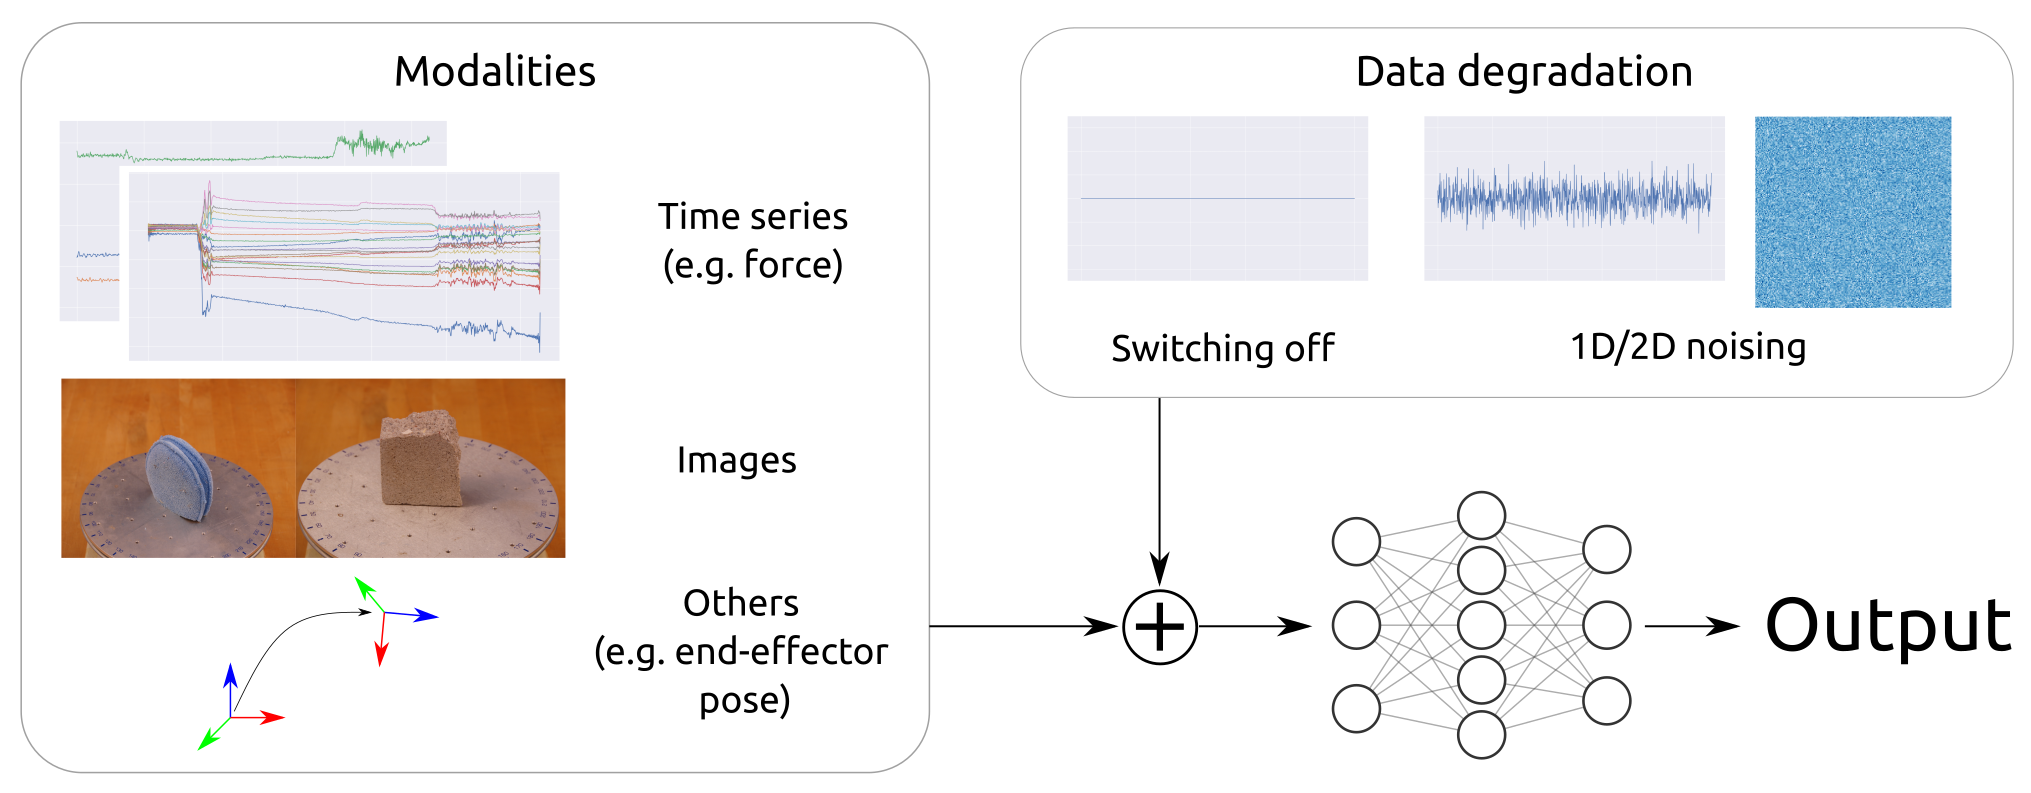
\includegraphics[width=0.95\textwidth]{images/on_robustness/overview.png}
    \caption{\Figure presents a general setup in conducted experiments. Different modalities subjected to different data degradation procedures were fed into the tested learning-based methods to evaluate their performance and robustness.}
    \label{fig:overall}
\end{figure}

The multimodal fusion in dexterous manipulation~\cite{see_feel_act, Lee_ICRA19} nowadays is an emerging field. However, the development of the field for such complicated robotic applications very often depends more on advances in sensors, such as skin-like measurement devices~\cite{gelsight_sensor, PointCloudsPlusTouch, biotac_sensor} than fusion algorithms themselves. The emphasis on research of multi-modal systems in the field of robotics is especially visible in areas like image segmentation~\cite{late_supervised, late_supervised_applied, hung2013orchard}, 3D reconstruction~\cite{fusing-senses-under-symmetry} and a tactile understanding~\cite{haptic_from_vision_and_biotac}. 

From the robotics perspective, the robustness of the multi-modal perception system against data corruption is of paramount importance. It can be achieved by finding interchangeable and complementary portions of information from different modalities in the input data stream. However, researchers mainly concentrated on establishing a benchmark in solved tasks rather than exploiting this complementarity. In state-of-the-art, there are very few examples of works where authors consider such interchangeability of modalities in the context of robustness, typical for real-life scenarios, noises, and sensor faults.

Multi-modal machine learning constitutes a scientific field of growing interest that brings many challenges. In~\cite{survey_morrency}, the authors have listed open questions that should find answers to advance state-of-the-art development. Firstly, how to represent the data (representation)? Then, how do we map knowledge from one modality to another (translation)? How do we find dependencies between heterogeneous modalities (alignment)? How do we join the multi-modal data stream together (fusion)? Finally, how to successfully transfer knowledge from training a model on one modality to another (co-learning)? Many data fusion techniques, such as the Kalman filter, Bayesian inference, and early fusion, can be found in the literature. Unfortunately, each solution is somewhat limited to low-dimensional or homogeneous data. Therefore, the proposed comparison does not cover them and focuses on the most flexible model-independent methods that can work with any data type. 

The following chapter investigates state-of-the-art data fusion methods based on artificial neural networks in robotics-oriented tasks. In the experiments, multiple scenarios were employed, like grasp outcome classification, haptic and visual fusion, haptic-only signals fusion, and multiple scenarios where the input modalities were subjected to noises.

\section{Related work}
\label{part:methods:fusion:rw}

\subsection{Data fusion approaches}
\label{part:methods:fusion:rw:approaches}

In the review~\cite{survey_morrency}, the authors separated the multi-modal fusion methods into subfields -- model agnostic and model-based. In the following work, experiments focused on the model agnostic methods because, typically, they are more general and widespread among roboticists. In the experimental section, chosen deep learning methods consist of three major categories of data fusion -- early (data-level), intermediate (feature-level), and late (decision-level)~\cite{survey_taylor}. Additionally, at least two of them might also be combined into one hybrid fusion method~\cite{survey_morrency}. In~\cite{Castanedo2013ARO}, the authors systematically divided different sensor fusion methods.

\paragraph{Early fusion} Generally, this type of fusion is based on combining information from different modalities at the very beginning of processing, \eg by concatenating input time series (if possible). This method enables the deep learning model to \textit{understand} low-level interactions between modalities and capture them together to produce meaningful features for further layers. However, a significant limitation exists for such approaches, \ie when input signals or low-level features from initial layers do not fit each other because they are heterogeneous. For example, it is not obvious how to incorporate 2D images with a 1D time series into one feature space. It would be possible to concatenate both modalities by flattening the 2D image into a 1D vector. However, it would cause a loss of information about each pixel's position and significantly decrease that modality's information gain. For that reason, an early fusion approach was not incorporated in the experimental section, as it generally does not apply to all data types in the comparison. 

\paragraph{Feature-level fusion} Combining different data representations at some high level of abstraction is a common practice in machine learning for data fusion. This technique allows for combining heterogeneous data from different modalities and lets the predictive model process joint representation. Among others, that type of fusion is popular in robotics-related areas such as object recognition~\cite{mid_object_recognition} and scene recognition~\cite{mid_scene_recognition}. In~\cite{mid_planning}, authors proposed a method for multi-modal data fusion applied to motion planning. In~\cite{Lee_ICRA19}, authors employed an early multi-modal fusion for the contact-rich manipulation task. Their compelling results were appreciated, and the authors received the best paper award at the International Conference on Robotics and Automation (2019). The authors of~\cite{mid_robust} proposed another method of feature-level fusion, where instead of concatenation, they fused only some random parts of feature vectors from different modalities. Alternative intermediate fusion approach~\cite{mid_LMF, mid_HPFN} use so-called Tensor Fusion Networks, which often appear in multi-modal sentiment analysis literature. However, to the best of the author's knowledge, they were not used in robotic applications yet. This type of deep learning model suffers from low computational efficiency; however, the follow-up work on the \acrshort{lmf} model in~\cite{mid_ELMF} further addressed this problem. The authors exploited a tensor decomposition to reduce the number of model parameters.

\paragraph{Late fusion} Generally, late fusion methods manage to work with any data type, similar to feature-level fusion methods. They do not combine information but only the outputs of separate models used to process different modalities. The work~\cite{Kittler98} presents an outstanding review of late fusion techniques. Authors of~\cite{late_ss, late_object_recognition, late_object_candidates} showed a typical plan of a late fusion. In~\cite{late_object_recognition,late_object_candidates}, the authors presented the late fusion method to process \acrshort{rgbd} data in object detection and discovery. The work~\cite{late_ss} showed the method to combine images and point clouds for the semantic segmentation of the urban environment for autonomous vehicles. In~\cite{late_uno}, the authors proposed a late fusion deep learning model, which took into account the influence of a data deterioration on the model's decision and used a noisy-or operation to integrate these decisions. The experimental section of the following work also investigates the robustness of fusion methods.

\paragraph{Hybrid fusion} This is an alternative approach to data fusion to the ones previously presented. It integrates information from different modalities at two or more levels. Authors of~\cite{late_supervised, late_supervised_applied} presented methods of such approaches for robust semantic segmentation in the outdoor environment for autonomous navigation. The authors proposed a convoluted mixture of deep experts that uses importance weights determined by a specialized gating network. This module, in turn, uses a feature-level representation of all modalities. The \acrfull{moe} can choose which modality should influence final segmentation more based on these weights.

\subsection{Fusion robustness}
\label{part:methods:fusion:rw:robustness}

Multi-modal and robotics-related literature very rarely considers fusion robustness. However, the author of the following thesis finds this problem urgent to solve regarding deploying an autonomous robot to the real world. Only several papers~\cite{mid_robust, late_uno, robust_gating, robust_lel, robust_pedestrians, robust_ugv} took into account the non-nominal conditions of a multi-modal fusion and provided some analysis of fusion robustness to data corruption. Such degradation could occur due to sensor noise, failure, or unexpected conditions like \eg electromagnetic influence of motors used in industrial areas. The method presented in~\cite{late_supervised} can potentially take into account mentioned data degradation and express its \textit{beliefs} in terms of the weighted model's decisions. However, the authors of this work did not elaborate more on that matter. Although one can find literature on the robustness of multi-modal fusion methods in robotics, it is noticeable that this area does not have any comprehensive and collaborative benchmark of fusion principles. 

\section{Proposed solution}
\label{part:methods:fusion:solution}

Typically, robots operating in the real world have at their disposal multiple onboard sensors like cameras, \acrshort{ft} measurement devices, \acrshort{lidar}s, \acrshort{imu}s, and others. They all play a significant role in robotic perception tasks, including haptic perception or scene reconstruction. However, they also produce a vital piece of information that needs to be efficiently processed to exhibit to ensure robustness against disturbances. As the volume and dimensionality of sensory-feedback increase, it might be troublesome to manually design a multi-modal data fusion system that can handle heterogeneous data. Recently, multi-modal machine learning became an emerging field with research focused mainly on analyzing vision and audio information. Although, from the robotics perspective, haptic sensations experienced from interaction with an environment are essential. The following experiments focused on four learning-based fusion methods and three datasets containing haptic signals, images, and robots’ poses. Tests related to grasp outcome classification, texture recognition, and -- most challenging -- a multi-label haptic adjectives classification based on haptic and visual data. Conducted experiments were focused not only on the verification of the performance of each method but mainly on their robustness against data degradation. Such degradation of sensory feedback might occur when the robot interacts with its environment. Additionally, the data augmentation technique was validated to increase the robustness of data fusion methods.

\section{Multi-modal fusion from the robotics perspective}
\label{part:methods:fusion:multimodal}

\subsection{Problem formulation}
\label{part:methods:fusion:multimodal:problem}

The following section investigated three types of recognition problems present in the literature. 

\paragraph{Binary classification of a grasp outcome} Let the $f_{binary} \colon \calS \mapsto \calC$ be a grasp outcome prediction function that assigns a Boolean value representing the predicted grasp outcome. It is based on sensory feedback from the set $\calS \colon \{s \in \Real^{3 \times n}\}$, where $3 \times n$ represents axes of the input data stream created with three tactile sensors mounted on a gripper.

\paragraph{Multi-class classification of textures} Let the $f_{single} \colon \calS \mapsto \calC$ be a grasp outcome prediction function that assigns a discrete value from the class counter-domain $\calC$ to a sensory measurement from the set $\calS \colon \{s \in \Real^{1}\}$ of signals registered while the unconstrained motion of a haptic sensor on a variety of surfaces.

\paragraph{Multi-label classification of haptic adjectives} Let $f_{multi} \colon \calS \mapsto \calH$ be a multi-label haptic classification function that assigns a subset of haptic adjectives from the set of strings $\calH = \{h_1, h_2, ..., h_m\}$ to a signal sample from the sensory domain $\calS \colon \{s \in \Real^{2\times n}\}$, where $2 \times n$ is a number of axes of the sensory feedback from two distinct sensors. Haptic adjectives assigned to each sample are not mutually exclusive, and each example might have an undefined number of haptic adjectives ranging from $1$ to $m$. In this task, the sensory domain $\calS$ contains heterogeneous data composed of \acrshort{rgb} images of household objects with associated 2 $\times$ 19-axes sensory feedback from the tactile sensor's electrodes.

Given the problem formulations above, the following components could be introduced:

\begin{itemize}
    \item an implementation and thorough comparison of four different deep learning methods for the fusion of multi-dimensional signals, including non-heterogeneous data -- Late, \acrshort{moe}, \acrshort{mid} and \acrshort{lmf}, that approximate functions $f_{binary}$, $f_{single}$, and $f_{multi}$ in respective tasks;
    \item research on the impact of the data deterioration and leading modalities on the predictions of each model in the aforementioned tasks;
\end{itemize}

\subsection{Multi-modal datasets}
\label{part:methods:fusion:multimodal:datasets}

\paragraph{\acrfull{bigs}} This is a dataset that consists of 2000 samples of sensory feedback from the BioTac~\cite{biotac_sensor} for the grasp-stability prediction. Haptic signals come from grasping three objects: a ball, a box, and a cylinder. Each was associated with the registered outcome -- a \textit{success} or a \textit{failure}. The authors of the following dataset used three bio-inspired BioTac sensors mounted on the fingers of a gripper and a \acrshort{ft} sensor mounted on the wrist to gather tactile sensory feedback. The experimental section of the following work shows the results of grasp outcomes based on the gripper's positions, orientation, and registered force signals. Each motion had a constant length by using the Fourier method to crop them. Eventually, each signal consisted of multi-dimensional time series with a length equal to 1053 time steps. Positions were 3-axis vectors, while orientation was 4-axis quaternion readings, and force readings were composed of 3-axis series. The training dataset for the cross-validation included 3197 signals from each modality, while the test set 801 such samples. All samples were independent of each other.

\paragraph{\acrfull{hatt}} The toolkit~\cite{penn_haptix} consists of 100 different textures photographed and presented as \acrshort{rgb} images. Each photo had associated normal force, acceleration, and position signals registered while the unconstrained motion of an impedance-type haptic device SensAble Phantom Omni~\cite{haptic_device}. \Table~\ref{tab:hatt_names} presents classes chosen for the experiments.

\begin{table}[H]
\centering
\caption{Textures from the \acrshort{hatt} chosen for the experiments.}

    \resizebox{\columnwidth}{!}{
\begin{tabular}{ccccc}
\toprule
ABS Plastic & Aluminum Foil & Aluminum Square & Artificial Grass & Athletic Shirt \\
\midrule
Binder      & Blanket        & Book             & Brick 1          & Brick 2        \\ \bottomrule
\end{tabular}
}
\label{tab:hatt_names}
\end{table}

Signals in the \acrshort{hatt} dataset register the motion of a haptic device's tool-tip on different surfaces for 10 seconds. The experimental section utilizes normal forces, acceleration, and velocity signals as input modalities. To combine 3-axis signals into a single axis, the authors of the dataset used the method DFT321~\cite{DFT321}. Hence, the experiments involve this flattened representation. The authors motivated the dimensionality reduction because humans cannot sense the direction of high-frequency vibrations~\cite{BELL199479}. The training dataset had 8000 signals, while the test set included 2000. All signals were fixed-length (200 time-steps each), while the number of samples inside each class remained balanced.

\paragraph{\acrfull{phac}} The experimental section regarding this dataset investigates the problem of multi-label classification of haptic adjectives. The authors of~\cite{CHU2015279} proposed an initial version of the \acrshort{phac} dataset, which has been updated in~\cite{haptic_from_vision_and_biotac}. The following dataset includes 53 objects photographed from 8 different views. Each photo received a corresponding haptic signal from squeezing an object with two BioTac sensors mounted on a gripper. Moreover, every example corresponds with several haptic adjectives used as labels. In the dataset, there were 24 haptic adjectives in total. \Figure~\ref{fig:phac_bar} presents the histogram of classes of the balanced dataset.

\begin{figure}[H]
\centering
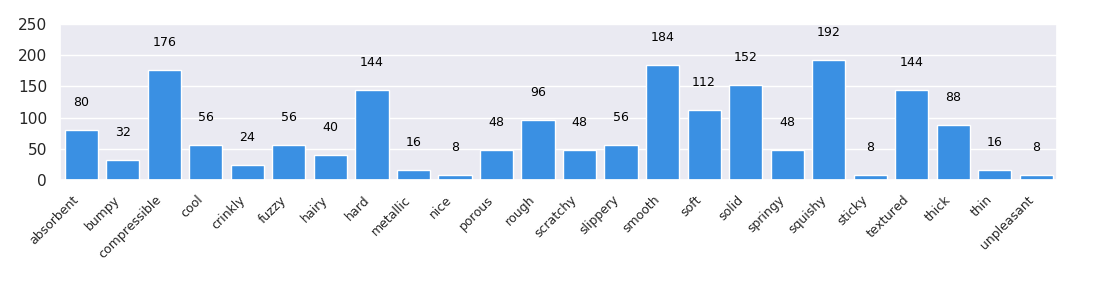
\includegraphics[width=0.98\textwidth]{images/on_robustness/barplot.png}
\caption{Occurrences of each adjective in the \acrshort{phac}.}
\label{fig:phac_bar}
\end{figure}   

In the experimental section, one had to ensure that the adjectives distribution remained fixed among train and test subsets. The iterative stratification method~\cite{iter_strat} enabled us to avoid over/under-representing haptic adjectives in the train/test subsets. The such imbalance would lead to a significant decrease in the prediction performance and misleading results. Hence one can find this procedure of paramount importance. An RBG image with the spatial resolution of 224 $\times$ 224 with two raw signals from 19-electrode arrays from both BioTac sensors represented one input sample. All time series remained fixed-length with 67 values each. Eventually, 265 data samples were in the training dataset, while 159 appeared in the test set.

\subsection{Fusion methods}
\label{part:methods:fusion:multimodal:approaches}

The literature review shows several model-agnostic data fusion techniques, but the experimental analysis incorporates four of them, as it was shown in~\Figure~\ref{fig:fusion}. Due to the simplicity and popularity of late and intermediate fusion, they inevitably appeared in the benchmark. The \acrfull{moe}~\cite{late_supervised} was another candidate for the experimental section. The proposed architecture was similar to the late fusion one, but it also can determine modality importance based on latent representations. The \acrfull{lmf} is a novelty in robotics, which appeared in the experimental analysis because of promising results in other areas, such as sentiment analysis. All of the chosen methods work on embeddings in the feature space. An encoder was a backbone for all models that transformed input signals into a 10-dimensional latent space. Each fusion method obtained $N$ latent vectors $L_1, L_2, \ldots, L_N$ fed to selected network architectures. Methods to data fusion examined in the experimental validation were presented schematically in \Figure ~\ref{fig:fusion} and described in detail below.

\paragraph{Late Fusion} Generally, that method's core operation principle is to process each input modality separately and combine predictions at the very end, assuming they are equally important. In ~\cite{Castanedo2013ARO}, authors described this merging process at the decision level. According to Dasarathy's fusion classification~\cite{Dasarathycls}, this approach is called the \acrfull{deideo}. Each latent vector was processed separately using neural networks in the experimental section. The overview shown in \Figure\ref{fig:fusion} illustrates these networks as arrows. This type of architecture was proposed to obtain predictions for each modality $p_1, p_2, \ldots, p_N$ in the form of logits. Next, these logits were summed up and transformed into class probabilities using a softmax function.

\paragraph{\acrfull{moe}} This method works according to the same principle as the Late Fusion, but it can also determine input modalities' importance weights through the gating network. That judgment was encoded in a vector $w$ representing weights, such that $\sum_{i=1}^{N} w_i = 1$. In contrast to the Late Fusion, corresponding weights influence predictions from modalities by multiplication. At the top, an \acrshort{mlp} takes all latent vectors and produces final predictions $w$. That architecture potentially facilitated a neural network to learn reactions to the input data degradation by assigning lower weights to the degraded modalities. On the other hand, if the data deterioration did not occur during a training phase, there was a possibility that the \acrshort{moe} would put too much emphasis on the modality affected by some noise during testing, which might result in false predictions.

\paragraph{\acrfull{mid}} The fusion of information carried by individual modalities happened by concatenating their representations in the latent space. This shared representation was processed further to obtain a prediction based on common features. Authors of~\cite{Castanedo2013ARO} presented a merging process at the feature level. According to Dasarathy's classification, this approach is the \acrfull{fifo}. That method lets a fusion model draw information from all modalities in the latent space and process them freely. The \acrshort{mid} method would also be able to gain some robustness to the data degradation during the training, as it could learn to reduce the impact of degraded modalities. However, in contrast to \acrshort{moe}, its robustness and decisions were not interpretable at any stage of calculations.

\paragraph{\acrfull{lmf}} This tensor-based approach for multi-modal fusion primarily focuses on revealing interactions between features extracted from different modalities. This technique aims to create some high-dimensional tensor-based representation by taking outer products over the uni-modal latent vectors $L_1, L_2, \ldots, L_N$. Then that representation linearly maps to the low-dimensional space using learned weights and biases. Fusion methods based on outer products typically suffer from computational inefficiency as tensor weights with the number of multiplications scale exponentially as the number of modalities. Nevertheless, the technique proposed by the authors of~\cite{mid_ELMF} does not use a high-dimensional weight tensor directly with the tensor representation of the data. The authors proposed decomposing tensor weights into $N$ sets of modality-specific factors to improve the method's efficiency. Such decomposition significantly reduced the number of computations, as it lets to map from feature space to predictions directly. Moreover, it does not require any more explicitly creating any high-dimensional tensors. 

\begin{figure}[H]
\centering
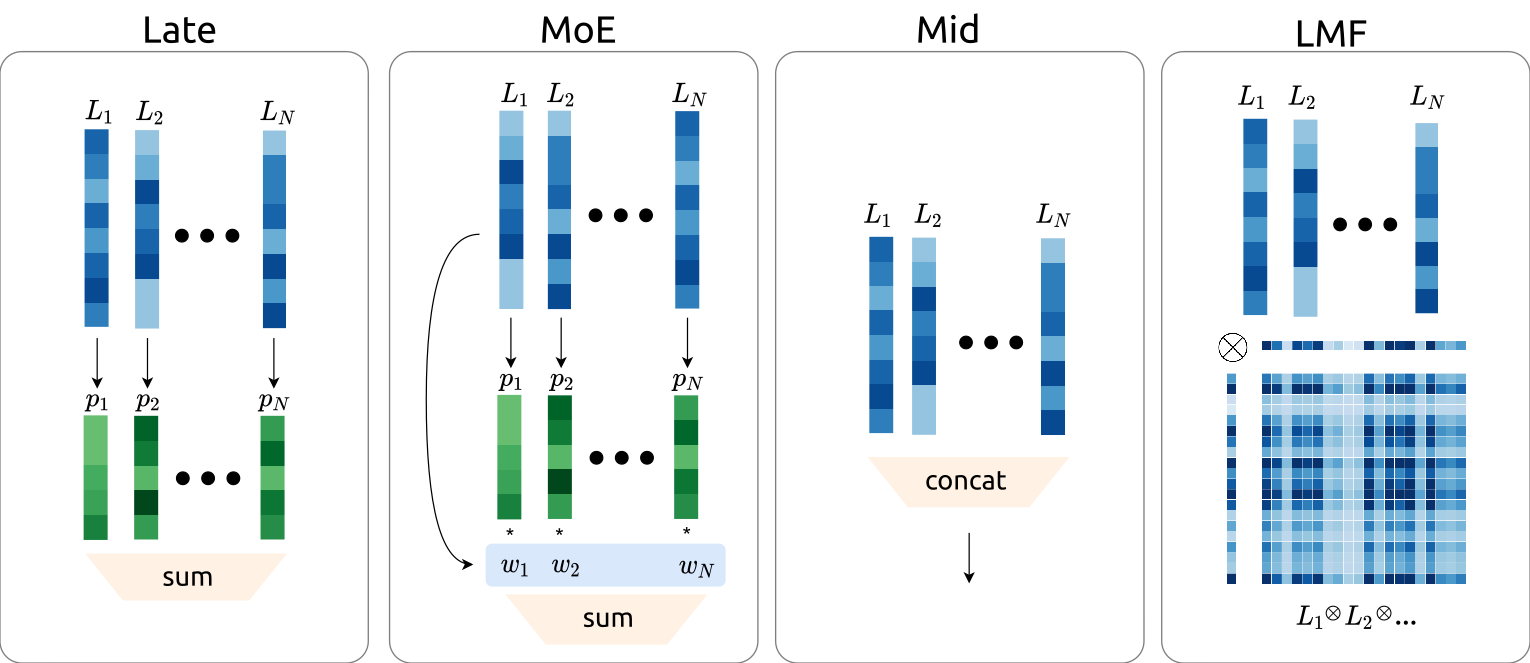
\includegraphics[width=0.98\textwidth]{images/on_robustness/arch.png}
\caption{Multi-modal fusion architectures used in experiments. From left: Late Fusion (Late), \acrfull{moe}, \acrfull{mid}, \acrfull{lmf}. Arrows represent transformations with neural networks, while $L_i, p_i, w_i$ denotes latent vectors, predictions, and trainable weight associated with $i$-th modality.}
\label{fig:fusion}
\end{figure}

\subsection{Discussion on chosen methods}
\label{part:methods:fusion:multimodal:models}

The four fusion methods presented in the following section have their advantages and disadvantages. Late Fusion is a relatively simple-to-implement method that does not require complex architectures and allows each modality to be processed independently. However, it assumes that all modalities are equally important, which may not be true in many scenarios. On the other hand, \acrshort{moe} gains an additional degree of freedom when learning the importance of each modality and adjusting its predictions accordingly. Still, it may assign too much weight to noisy or irrelevant modalities, leading to incorrect predictions. \acrshort{mid} allows the fusion model to draw information from all modalities in the latent space, which can improve robustness to data degradation during training. However, similar to \acrshort{moe}, its decisions are not interpretable again. Finally, \acrshort{lmf} aims to reveal interactions between features extracted from different modalities, but it suffers from computational inefficiency. The proposed decomposition in~\cite{mid_ELMF} significantly reduces the number of computations, but it still requires mapping from feature space to predictions directly. Thus, the choice of the fusion method should depend on the specific application's requirements and characteristics of the input modalities.

All models in the experimental section share a comparable number of learnable parameters. As datasets in the following experiments contained two heterogeneous types of data, \ie time series and images, 1D convolutional layers (Conv1D) followed by the \acrshort{lstm} units processed time-series, while the \acrshort{fc} at the top returned final predictions. Similarly, images were processed using 2D convolutional layers (Conv2D) with a few \acrshort{fc} layers on top.

Similar neural network architectures were used for the \acrshort{bigs} and \acrshort{hatt} datasets to produce latent vectors -- 3 $\times$ Conv1D layers with 64 filters of size 5 $\times$ 5 with stride equal to 2, followed by the \acrshort{lstm} layer with 32 units, and 2 \acrshort{fc} layers with 128 and 10 neurons respectively. However, in the case of the \acrshort{bigs} dataset, for \acrshort{mid}, Late, and the \acrshort{moe}, the number of units in the last \acrshort{fc} layer was changed to 2, as it was a binary classification. In the case of the \acrshort{moe} (for the \acrshort{bigs} and \acrshort{hatt}), the number of convolutional layers filters was reduced. This architecture uses an additional layer to produce $w_i$. This network for all datasets had the same architecture, namely, 3 $\times$ \acrshort{fc} layers with 128, 64, and $N$ units, where $N$ is the number of modalities. Similarly, in the \acrshort{mid} fusion to process the concatenated latent vectors into the predictions, but in the last layer, the number of units was equal to the number of classes.

In the experiments regarding the \acrshort{phac} dataset containing time series and images, heterogeneous data samples had to be processed together. Models used for time series had similar architecture as for \acrshort{bigs} and \acrshort{hatt} datasets, however with 24 neurons in the last \acrshort{fc} layer and 2 $\times$ Conv1D layers for all methods except the \acrshort{lmf}. While processing images, the neural network had 2$\times$ Conv2D layers with 64 filters of size 5$\times$5, stride 2, followed by 2 $\times$ \acrshort{fc} layers with 128 and 24 neurons. Again, except the \acrshort{lmf}, which had 10 neurons in the final layer.

The code used in the experimental section to create the following comparison is available online~\footnote{\url{https://bitbucket.org/m_bed/sense-switch/}}. It contains additional implementation details of fusion methods and the architectures of neural networks used in the experiments.

\part{Experimental verification}
\label{part:experiments}

\chapter{Material recognition}
\label{part:experiments:materials}

\section{Supervised stiffness estimation}
\label{part:experiments:materials:stiffness}

The main focus of this section is to introduce the results from the experiments on supervised stiffness estimation, which will be the subject of the subsequent section. I encourage readers to refer to the section \ref{part:methods:materials:stiffness} for formulating this topic.

\subsection{Comparison of architectures}
\label{part:experiments:materials:stiffness:comparison}

The experimental section contains the results of three types of neural networks tested using simulated signals to choose the best one for further experiments. Experiments on the performance of compared models focused on \acrfull{mae} defined as:

\begin{equation}
MAE(y_{true}, y_{pred}) = \frac{1}{n}\sum_{i=1}^{n}\left| y_{true_i} - y_{pred_i} \right|
\end{equation}

Where $y_{true}$ represents the true labels, $y_{pred}$ represents the predicted labels, $n$ represents the number of samples in the dataset, and $\left| \cdot \right|$ denotes the absolute value. The second evaluation metric was \acrfull{mape} defined as:

\begin{equation}
MAPE(y_{true}, y_{pred}) = \frac{100\%}{n}\sum_{i=1}^{n}\left|\frac{y_{true_i} - y_{pred_i}}{y_{true_i}}\right|
\end{equation}

\Table~\ref{tab:1st} presents values of \acrshort{mae} and \acrshort{mape} from the cross-validation. The objective of the comparison was to evaluate the performance of the proposed algorithms and choose the best-performing method for further experiments on shape generalization and to close the reality gap.

\begin{table}[hbt]
\centering
\caption{Comparison of three architectures according to \acrshort{mae}/\acrshort{mape} metrics. }
\begin{tabular}{c|c|c|c|c|c|c|}
\cline{2-7}
 & \multicolumn{2}{c|}{\textbf{\acrshort{cnn}}} & \multicolumn{2}{c|}{\textbf{ \acrshort{cnn}-\acrshort{lstm}}} & \multicolumn{2}{c|}{\textbf{\acrshort{cnn}-\acrshort{bilstm}}} \\ \hline
\multicolumn{1}{|c|}{\textbf{k-fold}} & \textbf{\acrshort{mae}} & \textbf{\acrshort{mape}} & \textbf{\acrshort{mae}} & \textbf{\acrshort{mape}} & \textbf{\acrshort{mae}} & \textbf{\acrshort{mape}} \\ \hline
\multicolumn{1}{|c|}{\textbf{I}} & 19,1 & 2,4 & 6,2 & 0,8 & 6,2 & 0,8 \\ \hline
\multicolumn{1}{|c|}{\textbf{II}} & 11,8 & 1,6 & 5,4 & 0,7 & 5,4 & 0,7 \\ \hline
\multicolumn{1}{|c|}{\textbf{III}} & 15,1 & 2,2 & 7,8 & 1,1 & 7,8 & 1,1 \\ \hline
\multicolumn{1}{|c|}{\textbf{IV}} & 14,6 & 1,9 & 6,7 & 0,9 & 6,7 & 0,9 \\ \hline
\multicolumn{1}{|c|}{\textbf{V}} & 18,1 & 2,1 & 6,2 & 1,0 & 6,2 & 1,0 \\ \hline
\multicolumn{1}{|c|}{\textbf{MEAN}} & 15,7 & 2,0 & 6,8 & 0,9 & \textbf{6,5} & \textbf{0,9} \\ \hline
\multicolumn{1}{|c|}{\textbf{SD}} & 2,9 & 0,3 & 0,9 & 0,2 & \textbf{0,7} & \textbf{0,1} \\ \hline
\end{tabular}
\label{tab:1st}
\end{table}

The experiments showed the performance of three types of neural networks in a stiffness parameter estimation based on inertial and sensory feedback. We were able to choose the best one for further analysis. Initially, experiments restricted all models to using only the simulation dataset without any real-world data samples. \Table~\ref{tab:1st} shows results from the cross-validation procedure on the simulation dataset to verify the consistency of the dataset and to find the best-performing model. The mean results of the \acrshort{mae}/\acrshort{mape} show the advantage of \acrshort{lstm} models in the stiffness estimation using raw inertial recordings. Firstly, the \acrshort{cnn}-\acrshort{bilstm} is more accurate in its predictions than \acrshort{cnn}, resulting in \acrshort{mae} of $6,5\frac{N}{m}$ and \acrshort{mape} of $0,9\%$, which means the improvement over $9,5\frac{N}{m}$ and $1,1\%$ achieved by the \acrshort{cnn}. Secondly, the resilience of the learning process also improved, and reduced deviations of errors obtained between cross-validation folds prove that statement. For \acrshort{cnn} a standard deviation of results is $2,9\frac{N}{m}$ \acrshort{mae} and $0,3\%$ \acrshort{mape}, while the \acrshort{cnn}-\acrshort{bilstm} reduced these metrics to $0,9\frac{N}{m}$ and $0,2\%$ respectively. Although the results for both recurrent models appear on the same level, the \acrshort{cnn}-\acrshort{bilstm} exhibited a slightly better performance resulting in a smaller \acrshort{mae}. It means a lower absolute error on average. Finally, any further experiments utilized that architecture.

\subsection{Shape generalization}
\label{part:experiments:materials:stiffness:estimation:generalization}

The experimental section includes more experiments concerning the simulation-only datasets to verify the capability of the \acrshort{cnn}-\acrshort{bilstm} in the stiffness estimation. They started from the cross-validation for chosen model and reported the \acrshort{mae}/\acrshort{mape} for three different datasets in \Table~\ref{tab:2nd}. Each test dataset consists of sensor readings from squeezing episodes of only one object to report outcomes on the shape-dependent regression. 

\begin{table}[hbtp!]
\centering
\caption{Results from experiments on the shape-invariant estimation of the stiffness parameter using \acrshort{cnn}-\acrshort{bilstm}.}
\begin{tabular}{|c|c|c|c|c|c|c|}
\hline
\multirow{3}{*}{\textbf{k - fold}} & \multicolumn{6}{c|}{\textbf{Dataset}} \\ \cline{2-7} 
 & \multicolumn{2}{c|}{\textbf{Ball}} & \multicolumn{2}{c|}{\textbf{Box}} & \multicolumn{2}{c|}{\textbf{Cylinder}} \\ \cline{2-7} 
 & \acrshort{mae} & \acrshort{mape} & \acrshort{mae} & \acrshort{mape} & \acrshort{mae} & \acrshort{mape} \\ \hline
\textbf{I} & 20,3 & 2,0 & 24,1 & 1,8 & 15,6 & 1,8 \\ \hline
\textbf{II} & 29,6 & 2,6 & 12,9 & 1,6 & 15,8 & 1,9 \\ \hline
\textbf{III} & 27,1 & 2,0 & 22,8 & 1,8 & 16,0 & 1,9 \\ \hline
\textbf{IV} & 21,8 & 2,1 & 17,7 & 1,6 & 18,4 & 1,9 \\ \hline
\textbf{V} & 19,3 & 2,0 & 24,4 & 1,5 & 20,8 & 1,9 \\ \hline
\textbf{MEAN} & 23,6 & 2,1 & 20,4 & \textbf{1,7} & \textbf{17,3} & 1,9 \\ \hline
\textbf{SD} & 4,5 & 0,3 & 5,0 & \textbf{0,1} & \textbf{2,2} & 0,0 \\ \hline
\end{tabular}
\label{tab:2nd}
\end{table}

\begin{figure}[hbtp!]
    \centering
    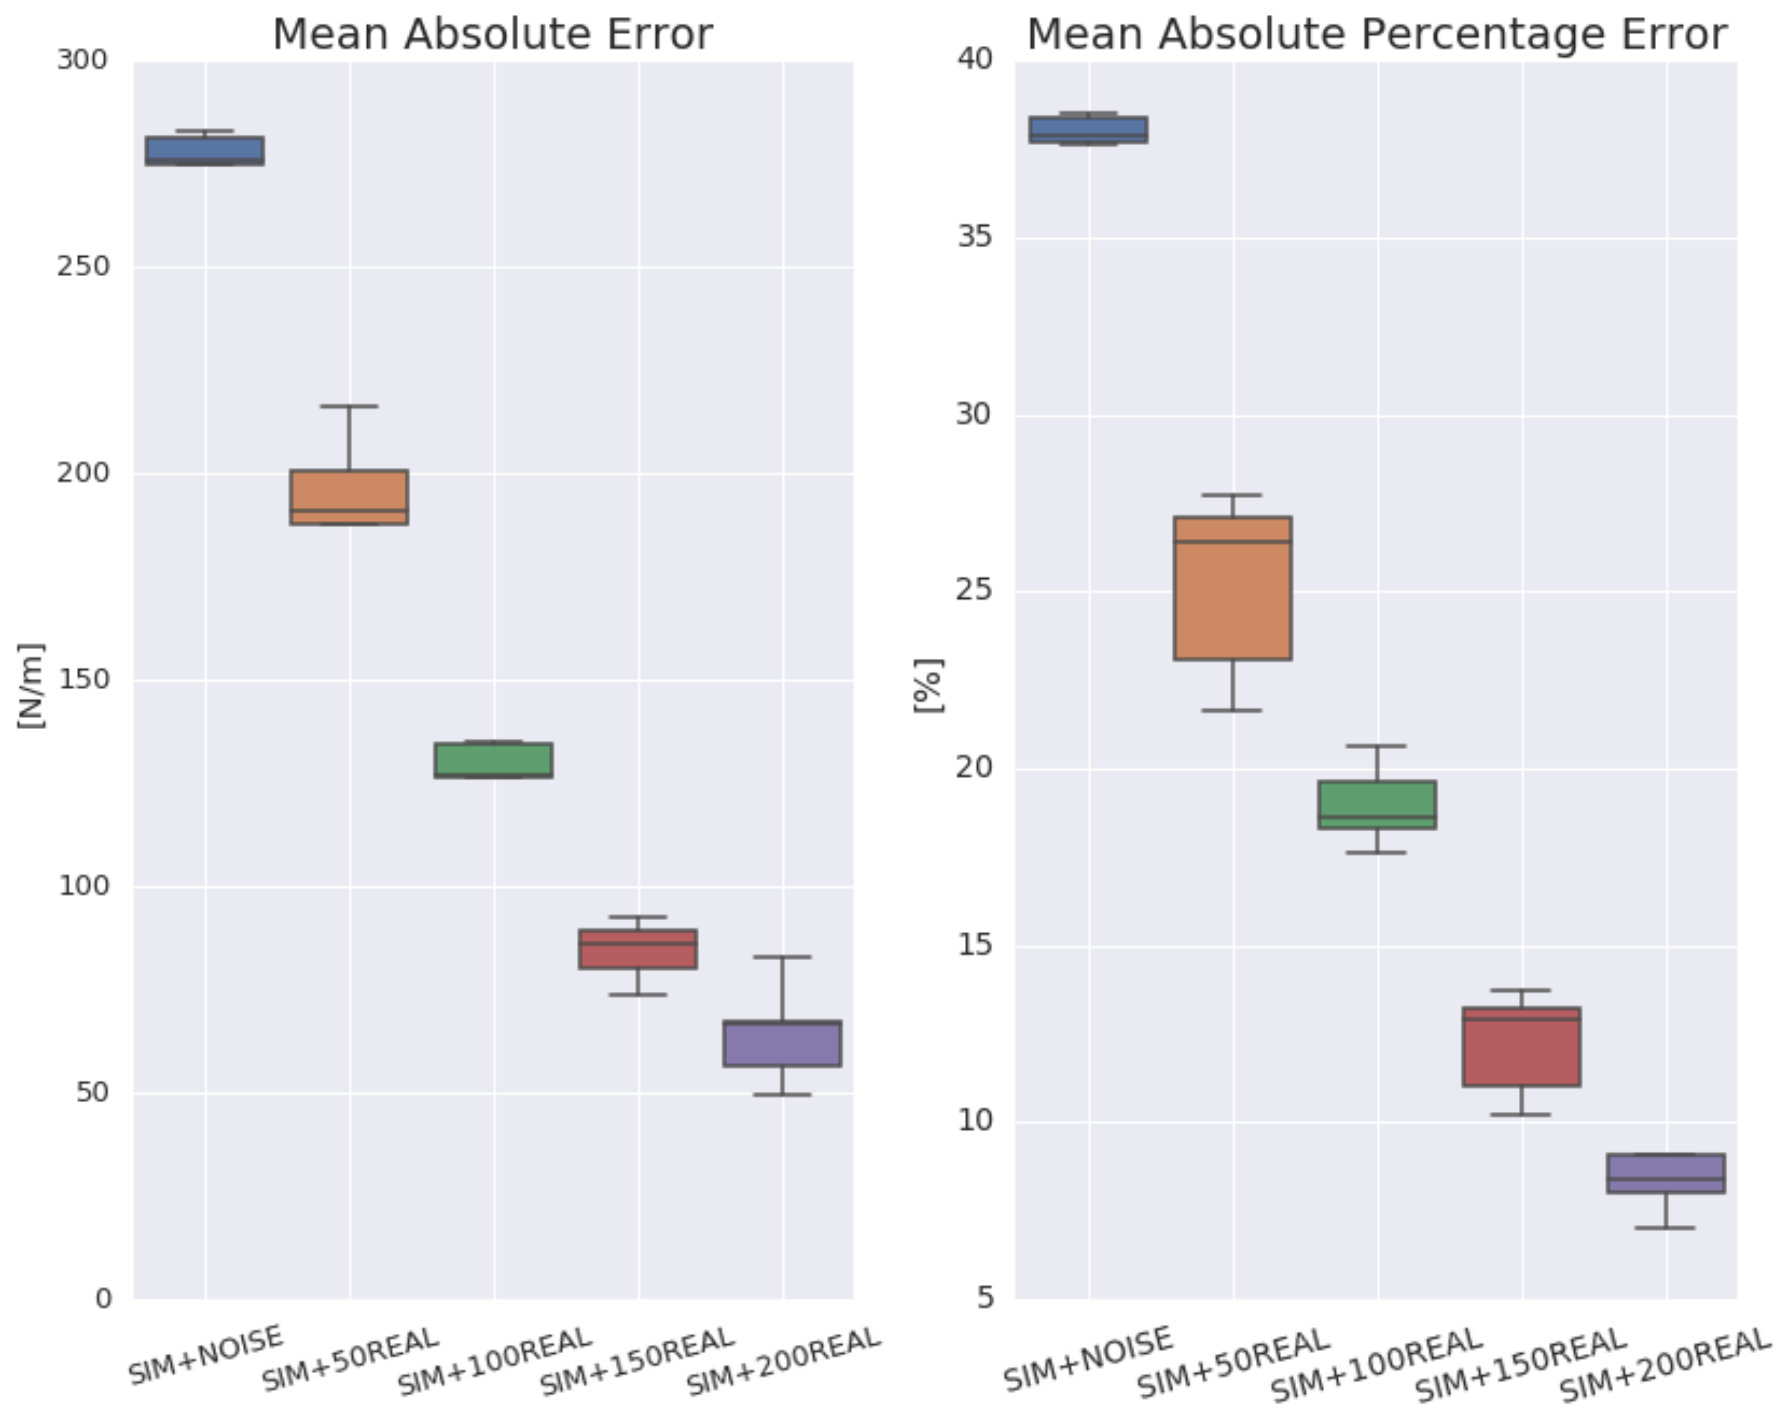
\includegraphics[width=0.8\textwidth]{images/gaining_sense_of_touch/MAE_MAPE.png}
    \caption{The box plot presents stiffness estimation performance metrics \acrshort{mae}/\acrshort{mape} obtained on real-world test dataset. The number of real-world data samples included in the training dataset increases while the test error decreases. Boxes represent successive experiments and consist of the five-number summary of the result (from the bottom of each box): minimum, first quartile, median, third quartile, and maximum value.}
    \label{tab:maemape}
\end{figure}

The generalization capability of the \acrshort{cnn}-\acrshort{bilstm} and verification of its performance on different types of objects need some additional experiments. \Table~\ref{tab:2nd} presents the \acrshort{mae}/\acrshort{mape} from testing the network on three separate datasets, each of which includes only one shape of an object while training all at once. The results show that the model performed well in the shape-invariant stiffness parameter prediction and generalized to different shapes. The cylinder-shaped instances apparently let the \acrshort{bilstm} achieve the lowest error than other shapes of $17,3\frac{N}{m}$ \acrshort{mae} and $1,9\%$ \acrshort{mape}. However, box objects gave smaller values of \acrshort{mae} ($20,4\frac{N}{m}$) than ball-shaped objects ($23,6\frac{N}{m}$), while looking at the \acrshort{mape}, the situation was the opposite, and some larger error was observed for boxes ($4,7\%$ / $2,1\%$). The model was inaccurate more often while predicting large stiffness values for boxes that resulted in the increased relative metric \acrshort{mape}. For spherical shapes, the estimation quality decreased to small values that gave increased absolute measure (\acrshort{mae}). 

\subsection{Closing the reality gap}
\label{part:experiments:materials:stiffness:estimation:gap}

\begin{table}[htbp!]
\centering
\caption{The table presents performance metrics \acrshort{mae}/\acrshort{mape} for best epochs from each of the cross-validation turns. Injecting even a small number of real-world sensor readings into the training resulted in a significant improvement in performance.}

\resizebox{\textwidth}{!}{%
\begin{tabular}{|l|c|c|c|c|c|c|c|c|c|c|c|c|}
    \hline
    \multicolumn{1}{|c|}{\multirow{3}{*}{\textbf{\begin{tabular}[c]{@{}c@{}}Experiment\\ Name\end{tabular}}}} & \multicolumn{10}{c|}{\textbf{k - fold}} & \multicolumn{2}{c|}{\textbf{MEAN}} \\ \cline{2-13} 
    \multicolumn{1}{|c|}{} & \multicolumn{2}{c|}{\textbf{I}} & \multicolumn{2}{c|}{\textbf{II}} & \multicolumn{2}{c|}{\textbf{III}} & \multicolumn{2}{c|}{\textbf{IV}} & \multicolumn{2}{c|}{\textbf{V}} & \multirow{2}{*}{\textbf{\acrshort{mae}}} & \multirow{2}{*}{\textbf{\acrshort{mape}}} \\ \cline{2-11}
    \multicolumn{1}{|c|}{} & \acrshort{mae} & \acrshort{mape} & \acrshort{mae} & \acrshort{mape} & \acrshort{mae} & \acrshort{mape} & \acrshort{mae} & \acrshort{mape} & \acrshort{mae} & \acrshort{mape} &  &  \\ \hline
    \textbf{sim + noise} & 281,3 & 37,7 & 275,0 & 38,5 & 275,6 & 38,4 & 282,7 & 37,6 & 256,6 & 37,9 & \textbf{274,2 $\pm$ 10,4} & \textbf{38,0 $\pm$ 0,4} \\ \hline
    \textbf{sim + 50 real} & 190,6 & 23,1 & 216,1 & 27,1 & 187,8 & 26,4 & 151,8 & 21,6 & 200,7 & 27,7 & \textbf{189,4 $\pm$ 23,8} & \textbf{25,2 $\pm$ 2,7} \\ \hline
    \textbf{sim + 100 real} & 134,6 & 20,6 & 108,3 & 17,6 & 134,9 & 19,6 & 126,8 & 18,6 & 126,6 & 18,3 & \textbf{126,2 $\pm$ 10,8} & \textbf{18,9 $\pm$ 1,2} \\ \hline
    \textbf{sim + 150 real} & 89,3 & 12,9 & 85,9 & 13,7 & 92,7 & 13,2 & 73,9 & 11,0 & 79,9 & 10,2 & \textbf{84,3 $\pm$ 7,5} & \textbf{12,2 $\pm$ 1,5} \\ \hline
    \textbf{sim + 200 real} & 66,9 & 9,1 & 49,3 & 7,0 & 82,6 & 10,9 & 67,4 & 8,4 & 56,6 & 8,0 & \textbf{64,6 $\pm$ 12,6} & \textbf{8,7 $\pm$ 1,5} \\ \hline
\end{tabular}
}
\label{tab:3rd}
\end{table}

In the haptic recognition of physical parameters, data from the physics simulator seemed to resemble the real-world \acrshort{imu} readings only to some extent. Although the results from \textit{sim + noise} tests were significantly worse than any of the \textit{sim + real} trail, the mean \acrshort{mape} $38\%$ suggests that the correspondence between the simulation-only and real-world signals exists. Another important note is that \acrshort{mae}/\acrshort{mape} values from each fold in the \textit{sim + noise} trial remained near to each other. The model's result was similar for the entire dataset, as it was equally balanced in the stiffness parameters range. However, we cannot consider the reality gap problem to be solved yet, because the greatest improvement appeared in the experiments with the real-world sensor readings in the training dataset. In \Figure\ref{tab:maemape}, one can observe the decreasing value of \acrshort{mae}/\acrshort{mape} metrics as the number of real data samples are added to the training dataset. The experimental section does not include the results from the training on the real-world data only, as they would be incomparable with other experiments due to the low variability of the stiffness coefficient. Additionally, the number of data samples would be too low to assess a fair comparison in a real-world scenario. The lowest \acrshort{mae}/\acrshort{mape} obtained in experiments on closing the reality gap were achieved for \textit{sim + 200 real} trial and were equal to $64,6\frac{N}{m}$ and $8,7\%$. However, in the \textit{sim + 50 real} experiment, the added number of real samples comprised only $1,2\%$ of the entire training dataset, but it gave the largest improvement among all experiments. The improvement was $84,8\frac{N}{m}$ and $12,8\%$ of the \acrshort{mae}/\acrshort{mape}.

\section{Unsupervised haptic recognition}
\label{part:experiments:materials:unsupervised}

The main focus of this section is to introduce the results from the experiments on unsupervised haptic recognition. I encourage readers to refer to the section \ref{part:methods:materials:dec} for formulating this topic.

\subsection{Clustering of force measurements from the Touching dataset}

The following experiments compare unsupervised learning methods in the clustering assignment of 3-axis force readings. These were gathered in equally distributed episodes of touching different materials lying on the hard surface. \Figure\ref{fig:unsupervised_touching_barplot} shows the benchmark of different models tested on the Touching dataset. One can observe that \acrshort{dec} methods outperformed other, more classical approaches, showing almost 60\% of clustering accuracy, 0.7 normalized mutual information score, and 0.65 purity. Only a slight improvement was observed for the \acrshort{dec} variant that clustered embeddings produced by the autoencoder. These were improvements achieved: 2.7\%, 0.3\%, and 3.1\% accordingly.

\begin{figure}[htbp!]
    \begin{center}
        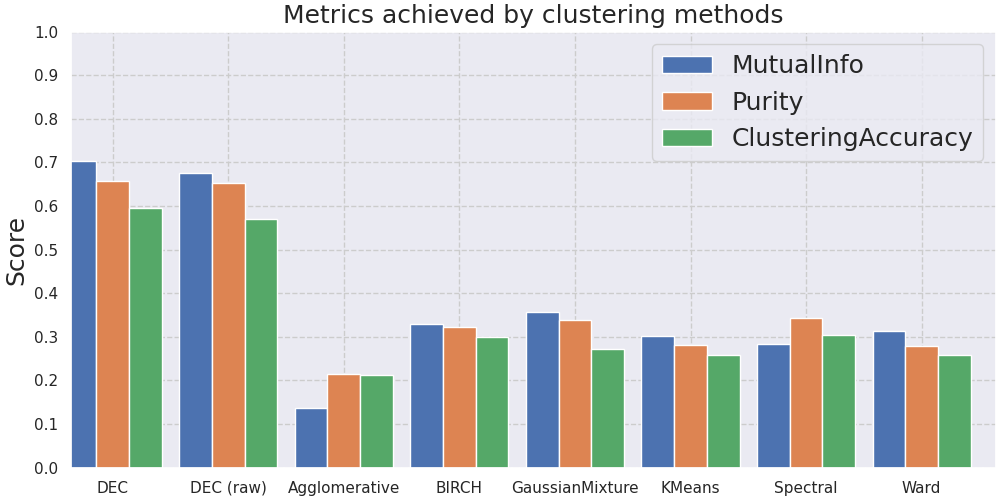
\includegraphics[width = \columnwidth]{images/unsupervised/touching_bar_plot.png}
        \caption{Evaluation metrics obtained for the clustering assignment of the Touching dataset.}
        \label{fig:unsupervised_touching_barplot}
    \end{center}
\end{figure}

Classical machine learning methods for the clustering task did not meet any requirements of real-world deployment, achieving clustering accuracy below 20\%, while one of them - the Agglomerative Clustering method, was less than 10\%. It means these methods are unsuitable for real-world time series from our experiments. Time dependencies, high signal noise typical for robotic applications, and a relatively small dataset prevent them from being useful for the clustering task.

However, one can observe that force measurements in the Touching dataset might not correctly describe touched material because they all lay on a hard surface. Hence, thin fabrics, like, \eg linen bags, could take on the properties of the ground and become hard to recognize without supervision. On the other hand, hard materials, like fabric or plastic, might be difficult to differentiate based only on force measurements. That is why the Touching dataset was challenging. More experiments on unsupervised haptic recognition were needed using another dataset - preferably the one that isolates touched objects from the ground and ensures measurements from different directions to gain more insight into the object's physics. 

\subsection{Experiment design importance - BioTac dataset}

More experiments were needed to verify the usefulness of unsupervised learning methods in haptic recognition. \Figure\ref{fig:unsupervised_biotac_barplot} shows the comparison of chosen methods for clustering haptic measurements from the BioTac sensors. Again, both \acrshort{dec} variants outperformed classical approaches by a large margin in all performance metrics, which proves that classical methods are not the proper choice for such a task.

However, all metrics of both \acrshort{dec} methods significantly improved compared to the experiments conducted on the Touching dataset. For the \acrshort{dec} clustering latent vectors from the autoencoder, the mutual information score achieved over 0.9, which means that the proposed clusters are statistically similar to the proper labels. That result is impressive, considering that there were 51 different classes in the dataset. Similarly, the purity score exceeding 0.8 shows that predicted clusters are homogeneous and mainly contain one object type each. Finally, the clustering accuracy of 79\% shows that \acrshort{dec} clustering strategies of the unsupervised haptic recognition task are suitable for robotics applications demanding such a functionality. This accuracy score is calculated by finding the optimal assignment of predicted labels to clusters using the Hungarian algorithm and then computing the ratio of correctly assigned labels to the total number of samples. Unsupervised accuracy does not require the notion of classes as in supervised learning, and can achieve 100\% when all samples from each true label fall into separate clusters.

\begin{figure}[htbp!]
    \begin{center}
        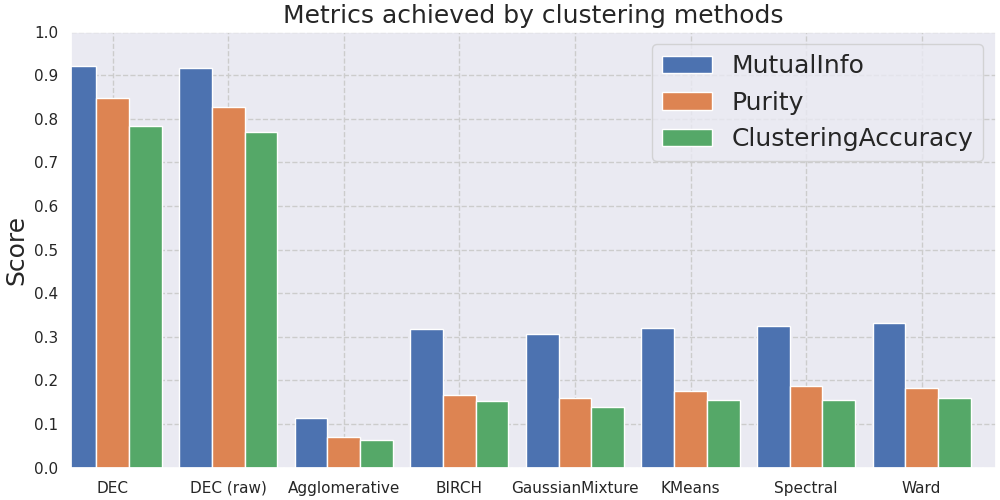
\includegraphics[width = \columnwidth]{images/unsupervised/biotac2_bar_plot.png}
        \caption{\acrshort{bigs2} consists of sensor measurements collected at a single time step, allowing \acrshort{dec} to operate on raw data without any encoding. This \Figure displays evaluation metrics for the benchmark methods in the clustering assignment.}
        \label{fig:unsupervised_biotac_barplot}
    \end{center}
\end{figure}

Again, similarly to the experiments using the Touching dataset, \acrshort{dec} variant clustering latent vectors achieved slightly better results than the one working on raw measurements, exceeding its mutual information score, purity, and clustering accuracy by 0.5, 0.1, and 1.3\%, respectively.

\section{Discovering tactile dimensions - silhouette test}

A human's sense of touch might carry complex information about the touched surface - not only about its hardness but also the type of texture, shape, or temperature. These factors might be categorized into \textit{tactile dimensions} that comprise the psycho-physical perception of the world. In~\cite{review_on_haptic_perception}, authors conducted extensive experiments that yielded a definition of these categories: macro, fine roughness, warmness/coldness, hardness/softness, and friction. In the following experiments, the objective was to find the optimal number of clusters - if tactile dimensions exist, the optimal number of revealed sets would equal the number of dimensions. Thus, the experiment would prove or refute the thesis posed by the authors of~\cite{review_on_haptic_perception}. Typically, we use silhouette analysis to find the optimal number of clusters in the clustering assignment. The technique involves calculating the silhouette coefficient (see \ref{part:methods:materials:classification:metrics}) for each cluster sample, which measures how closely it matches its cluster compared to other groups. The silhouette coefficient ranges from -1 to 1, with a high value indicating that the example is well-matched to its cluster and a low value indicating that the sample is poorly matched and may be better suited to a different set. 

Previous tests showed that only the \acrshort{dec} was suitable for the silhouette analysis on the \acrshort{bigs2} dataset. However, that method required different numbers of expected clusters before the training, so it started from scratch for every trial. These experiments involved \acrshort{dec} variant working on latent vectors. \Table\ref{tab:silhouette_scores} presents silhouette scores obtained after consecutive training procedures. The highest score achieved model grouping data samples into three groups. 

\begin{table}[htbp!]
\centering
\begin{tabular}{c|cccccc}
                 & \multicolumn{6}{c}{Num. of clusters}          \\
                 & II    & III   & IV    & V     & VI    & VII   \\ \hline
Silhouette score & 0.467 & \textbf{0.475} & 0.406 & 0.301 & 0.300 & 0.264
\end{tabular}
    \caption{Silhouette score for the \acrshort{dec} for different numbers of clusters.}
    \label{tab:silhouette_scores}
\end{table}

\Figure\ref{fig:silhouette_analysis} visualizes embeddings using T-SNE and silhouette scores for every sample in the dataset. The model trained to group data into three clusters achieved the highest result. BioTac sensor is one of the most sophisticated haptic sensors on the market. However, compared to the human's fingertip, its 24 sensing electrodes might be too sparsely placed to recognize an object's macro and roughness properly, so the clustering strategy is based on other tactile dimensions -- warmness, hardness, and friction. That result partially proves the existence of tactile dimensions.

\begin{figure}[htbp!]
    \begin{center}
        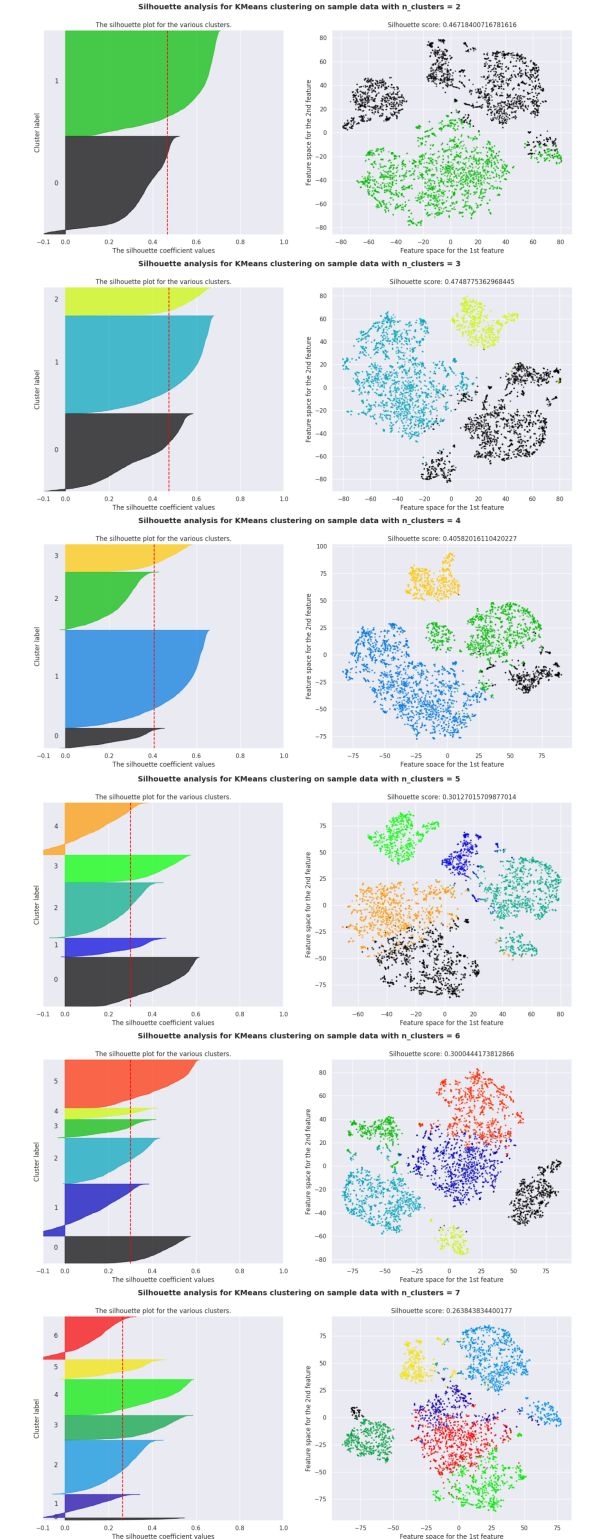
\includegraphics[width = 0.6\columnwidth]{images/unsupervised/silhouette.png}
        \caption{Silhouette test for every sample in the \acrshort{bigs2} dataset next to the visualization of embeddings using the T-SNE method.}
        \label{fig:silhouette_analysis}
    \end{center}
\end{figure}


\chapter{Terrain classification}
\label{part:experiments:terrain}

\section{Terrain classification using Transformers}
\label{part:experiments:terrain:haptr}

The main focus of this section is to introduce the results from the experiments on terrain classification for walking robots. I encourage readers to refer to the section \ref{part:methods:terrain:haptr} for formulating this topic.

\subsection{Real-life requirements for the terrain classification}
\label{part:experiments:terrain:requirements}

In the vast majority of the research articles, overall accuracy is the state-of-the-art metric describing the performance of the supervised terrain recognition algorithm. However, when the distribution of classes in the dataset is not uniform, this measure will be skewed in favor of over-represented categories. 

In the real world, an autonomous robot has to deal with numerous terrain types that naturally occur with different frequencies and want to acquire a reliable performance in all the considered terrains. To verify that classification algorithms are robust enough to operate in the real world, the experimental section presents a criterion of minimal accuracy $\textit{Acc}_{min}$:
\begin{equation}
    \textit{Acc}_{min} = \min_i(\textit{Acc}_i),
\end{equation}
where $\textit{Acc}_i$ is the accuracy for an $i$-th terrain type. The goal of the $\textit{Acc}_{min}$ measure is to capture the classifier's performance on the most challenging terrain type.

The accuracy metric represents the system's ability to recognize the terrain but does not capture if it is viable to be deployed and used on a real legged robot. This chapter argues that the classification method must have a low computational burden and fast inference time for the robot to adapt its gait in real-time and prevent any possible damage. As each walking robot is different, the overriding assumption is that an inference time below 10~ms would satisfy these needs and be estimated based on the typical frequency of the control loops of the legs reaching hundreds of times per second. The neural network size should be as small as possible as a genuine autonomous robot needs \acrshort{gpu} capabilities for a range of other tasks, \eg object detection or segmentation. Apart from the general accuracy, we should also consider the accuracy of the most challenging terrain, model size, and inference time to determine the best classification method for the terrain classification task. 

\subsection{Accuracy evaluation on the Poznan University of Technology ANYmal dataset}
\label{part:experiments:terrain:accuracy}

In this section, to compare the \acrshort{haptr} with the public results, the \acrshort{putany} dataset was split into train/test subsets. The test data came from a different run than the samples used for training. \Table~\ref{tab:dl_results} presents the results obtained by the classical algorithms (\acrshort{knn}-\acrshort{dtw}, \acrshort{rocket}), classical deep learning solution (\acrshort{tcn}), transformer-based approaches (\acrshort{haptr}, \acrshort{haptr}2), and the state-of-the-art \acrshort{cnn}-\acrshort{rnn}.

\begin{table}[htbp!]
\centering

\caption{\elsevier{2022} The accuracy comparison measured on the test set of the \acrshort{putany} dataset.}

\begin{tabular}{ccccccc}
\hline
Method                 & Variant  & $Acc$ [\%] & $Acc_{min}$ [\%] \\ \hline
\acrshort{knn}-\acrshort{dtw}                & -       & 74.0 & 54.4 (\acrshort{pvc}) \\ 
\acrshort{rocket}                 & -       & 84.9 & 47.3 (\acrshort{pvc}) \\ \hline{}
\multirow{3}{*}{\acrshort{tcn}}   & \textit{Light}     & 84.5 & 68.7 (Art. grass)\\
                       & \textit{Base}      & 86.9 & 65.1 (Art. grass)\\
                       & \textit{Large}     & 87.5 & 72.3 (Art. grass)\\ \hline
\multirow{3}{*}{HAPTR} & \textit{Light}     & 83.3 & 56.6 (Art. grass)\\
                       & \textit{Base}      & 90.3 & 80.7 (Art. grass)\\
                       & \textit{Large}     & 91.7 & 74.7 (Art. grass)\\ \hline
\multirow{3}{*}{HAPTR2} & \textit{Light}   & 91.7 & 80.7 (Art. grass)\\
                       & \textit{Base}      & 92.2 & 81.9 (Art. grass)\\
                       & \textit{Large}     & 92.7 & 81.9 (Art. grass)\\ \hline
\acrshort{cnn}-\acrshort{rnn}~\cite{KubaRNN}             &        & 93.0 & 86.7 (Art. grass)\\ \hline                      

\end{tabular}
\label{tab:dl_results}
\end{table}

The results achieved on the test set indicate that deep learning methods (\acrshort{tcn}, \acrshort{haptr}, \acrshort{haptr}2, \acrshort{cnn}-\acrshort{rnn}) generally achieve better accuracy than any of the classical approaches (\acrshort{knn}-\acrshort{dtw}, \acrshort{rocket}). The most fundamental and universal \acrshort{knn}-\acrshort{dtw} method performed the worst -- $74\%$, while the \acrshort{rocket} classifier improved its result to $84.9\%$. The overall satisfactory accuracy of the \acrshort{rocket} came with a poor ability to perform on the most challenging terrain (\acrshort{pvc}) of $47.3$, which might be inadequate to complete the necessary gait adaptation. Among the deep learning methods, the different variants of the \acrshort{haptr} outperformed the classical approach (\acrshort{tcn}). Similarly, the improved \acrshort{haptr}2 exceeded the result of the \acrshort{haptr}. For all of these methods, we reported that increasing a network's size improved its accuracy and also improved $\textit{Acc}_{min}$. Nevertheless, neither of the presented solutions could overcome the state-of-the-art \acrshort{cnn}-\acrshort{rnn} solution that reported the best accuracy of $93.0\%$ with the best $\textit{Acc}_{min}=86.7\%$.

This comparison shows the model's accuracy without cross-validation (CV) as opposed to comparable works of~\cite{KubaRNN} and~\cite{Ahmadi2021}. The following experiments required an independent test set to truly measure the performance of a network in a setup resembling a real-world operation. Reporting results from cross-validation can still provide valuable information, such as the variance of the performance estimates. However, it may give a less accurate estimate of the model's performance on new data. The accuracy comparison comes from an experiment using n-fold CV, and the test accuracy originates from using an independent testing sequence to verify this claim. All analyzed methods achieved accuracy lower by several percentage points using testing sequence than n-fold CV. Most notably, even the best-performing \acrshort{cnn}-\acrshort{rnn} reported $94.1\%$ when using CV~\cite{KubaRNN} while we were only able to obtain $93.0\%$ on the independent testing sequence.

\subsection{Accuracy depending on the model size}
\label{part:experiments:terrain:modelsize}

Typically, the most extensive predictive models achieve the best performance on the chosen dataset. They are often too large to be trained or used in practical scenarios, thus being considered a dedicated solution for a particular dataset. Therefore, the applied deep learning community is currently more interested in efficiently formulating artificial neural networks and proving that these architectures are more capable than their predecessors with the same number of parameters in the case of EfficientNetV2~\cite{efficientnetv2}. \Figure\ref{fig:params} presents a similar analysis with the accuracy presented in a function of the number of learnable parameters. The \acrshort{knn}-\acrshort{dtw} was omitted in this analysis as it is a non-learnable method.

\begin{figure}[htbp!]
    \begin{center}
        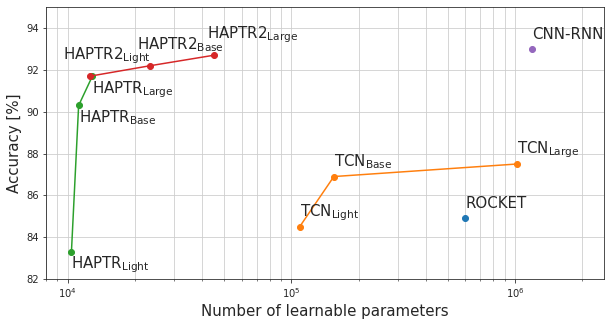
\includegraphics[width = \columnwidth]{images/transformers/parameters.png}
        \caption{\elsevier{2022} The accuracy as a function of a number of parameters reveals the efficiency of the applied method. Notice that the axis of parameters is in the logarithmic scale. In this context, \acrshort{haptr}2 significantly outperforms other algorithms.}
        \label{fig:params}
    \end{center}
\end{figure}

In \Figure ~\ref{fig:params}, one can notice that the \acrshort{cnn}-\acrshort{rnn} achieved the highest accuracy, but it came with a price of its substantial number of learnable parameters. This method would not fit the restricted computational resources of a mobile robot setup. Still, it appears to be more efficient than the classical \acrshort{tcn} approach or even less efficient \acrshort{rocket}. Both transformer-based solutions, \acrshort{haptr} and \acrshort{haptr}2, require an order of magnitude fewer parameters to achieve performance similar to \acrshort{cnn}-\acrshort{rnn}. The \acrshort{haptr}2 contains more learnable parameters than the \acrshort{haptr}, as it contains an additional attention mechanism but achieves significantly better results than the \acrshort{haptr}. The introduction of such a module improved an internal representation of the input signal, which enabled better classification. Therefore, it is reasonable to use the family of attention-based solutions together with convolutional layers whenever the efficiency of the methods is the primary factor. Typically, convolution as a mathematical operation preserves high-frequency features, such as peaks in time series. However, the softmax function inside attention modules flattens the resulting representation and behaves more like a low-frequency filter~\cite{park2022how}. Its output becomes complementary with a convolution operation. The combination of both layers together yielded better robustness and classification accuracy.

\subsection{Inference time evaluation}
\label{part:experiments:terrain:inferencetime}

The number of learnable parameters determines the ability to deploy networks in resource-constrained environments. Still, it might be challenging to compare networks properly as it depends on the chosen hardware setup. The network's size also impacts the training time, which we might consider irrelevant, as we trained them offline. The remaining aspect of a chosen model size is inference time. An inference time determines the real-world viability of the proposed solution, as having a prolonged processing time might be unacceptable from the perspective of the control that has been done based on this result. The  \Table~\ref{tab:dl_inference} presents the processing times on \acrshort{cpu} (Intel i7-9750H @ 2.600GHz) and \acrshort{gpu} (NVIDIA GeForce GTX 1660 Ti Mobile) for all of the considered methods.

\begin{table}[ht]
\centering

\caption{\elsevier{2022} Inference time for a single sample for evaluated terrain classification algorithms.}

\begin{tabular}{cccc}
\hline
Method                 & Variant &  \acrshort{cpu} [ms] &  \acrshort{gpu} [ms] \\ 
 \hline
\acrshort{knn}-\acrshort{dtw}              &            & $1619.86 \pm 11.11 $               & -- \\ 
\acrshort{rocket}              &            &  $180.62 \pm 13.05 $                   &  -- \\\hline 
            

\multirow{3}{*}{\acrshort{tcn}}   & \textit{Light}       &  $1.37\pm0.29$ &  $1.86\pm0.05$ \\
                       & \textit{Base}      &  $2.97\pm0.24$ & $3.37\pm0.04$ \\
                       & \textit{Large}    &  $16.82\pm0.91$ & $6.43\pm0.06$ \\ \hline
\multirow{3}{*}{HAPTR} & \textit{Light}       &  $1.43\pm0.09$     &    $1.61\pm0.15$ \\
                       & \textit{Base}      &  $2.91\pm0.22$    &    $2.73\pm0.06$ \\
                       & \textit{Large}     &  $5.60\pm0.59$ & $4.87\pm0.15$\\ \hline
\multirow{3}{*}{HAPTR2} & \textit{Light} & $1.38\pm0.03$ & $1.53\pm0.11$ \\
                         & \textit{Base}  & $2.25\pm0.05$ & $2.13\pm0.05$ \\
                         & \textit{Large} & $3.99\pm0.09$ & $3.39\pm0.05$ \\ \hline
\multirow{1}{*}{\acrshort{cnn}-\acrshort{rnn}}~\cite{KubaRNN} &        &   $11.68\pm0.83$     &       $30.60\pm5.30$          \\ \hline
\end{tabular}

\label{tab:dl_inference}
\end{table}

Initially, let us consider a mobile robot equipped with a powerful \acrshort{cpu} but no \acrshort{gpu}. \Figure~\ref {fig:infer_acc_cpu} presents results of the accuracy comparison as a function of mean inference times. In such a case, the \acrshort{knn}-\acrshort{dtw} method performed poorly, and it took over 1600 ms to reach the desired classification result. This inference time was obtained for a selected size of training samples but would even increase if we added more signals, making this approach slow and unscalable for any real-world deployment. Nevertheless, the other non-deep learning \acrshort{rocket} showed results in 180~ms, which is too long to implement any reaction-based behavior based on the obtained results. Deep-learning-based methods exhibited significantly lower inference times. The \acrshort{haptr}2 reported the shortest \acrshort{cpu} inference time. But it is also worth noting that the \acrshort{haptr} in all variants and the \acrshort{tcn} in \textit{Light} and \textit{Base} variants meet the previously stated requirement of 10~ms terrain classification time. In this comparison, the state-of-the-art \acrshort{cnn}-\acrshort{rnn} solution did not meet our criteria, exceeding the set threshold for the inference time, thus making it not suitable for a real-time operation.

\begin{figure}[htbp!]
    \begin{center}
        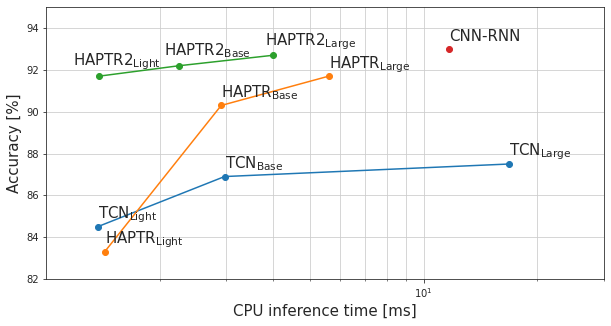
\includegraphics[width = \columnwidth]{images/transformers/cpu.png}
        \caption{\elsevier{2022} The accuracy of deep learning models as a function of a mean inference time on \acrshort{cpu}. Notice that the axis of an inference time is in a logarithmic scale.}
        \label{fig:infer_acc_cpu}
    \end{center}
\end{figure}

\Table~\ref{fig:infer_acc_gpu} shows the results for a robot equipped with a \acrshort{cpu}, and the trade-off between accuracy and inference time on a \acrshort{gpu}. Classical methods (\acrshort{knn}-\acrshort{dtw} and \acrshort{rocket}) did not appear in the plot, as their implementations were not \acrshort{gpu}-friendly. One can observe similar trends for deep-learning solutions to the processing performed on a \acrshort{cpu}. Surprisingly, no acceleration was observed in most cases when using a \acrshort{gpu}. In the experiments, we defined the inference time as the total time needed for calculations and related tasks. It includes the time of transmitting data between the main memory and \acrshort{gpu}'s memory. This overhead is present in all the measurements of inference time included in the comparison. The reduced time is visible only for the \acrshort{tcn} in \textit{Large} that decreased below the accepted threshold. Much to the surprise, the inference time of the \acrshort{cnn}-\acrshort{rnn} increased on the \acrshort{gpu}. The possible explanation would be insufficient optimization of the \acrshort{rnn} model on this particular \acrshort{gpu} architecture. Another probable reason would be sequential processing in recurrent units, which cannot fully utilize a \acrshort{gpu} computational power -- \acrshort{gpu}s were designed primarily for parallel processing. Eventually, the \acrshort{haptr}2 appeared to be the most efficient method based on the accuracy and the inference time on a \acrshort{cpu} or \acrshort{gpu}.

\begin{figure}[htbp!]
    \begin{center}
        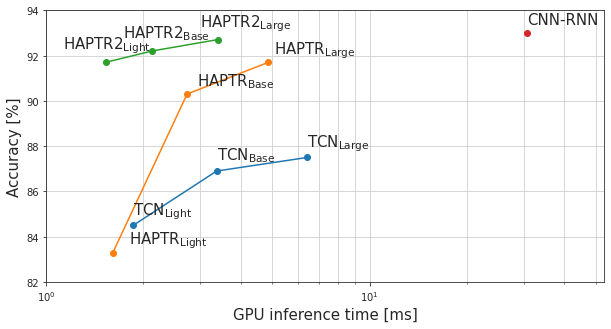
\includegraphics[width = \columnwidth]{images/transformers/gpu.png}
        \caption{\elsevier{2022} The accuracy as a function of a mean inference time on \acrshort{gpu}. The axis of time is in the logarithmic scale. }
        \label{fig:infer_acc_gpu}
    \end{center}
\end{figure}

\subsection{The choice and analysis of the best solution}

Based on the results presented in the previous subsections, it becomes evident that the choice of the terrain classification method should not be based solely on its accuracy result. The decision on this topic should also be dictated by factors important to the real-world deployment, such as minimal classification accuracy on the most challenging terrain, model size, and its inference time on the target hardware. Overall, the chapter indicates that the \acrshort{haptr}2 family provides the best efficiency and is regarded as the best choice for the trade-off between the accuracy and remaining requirements. Therefore, for further analysis, \acrshort{haptr}2\textsubscript{Light} was chosen. Consequently, \Figure\ref{fig:confusion} presents the confusion matrix of this approach to provide more insight into observed performance.

\begin{figure}[htbp!]
    \begin{center}
        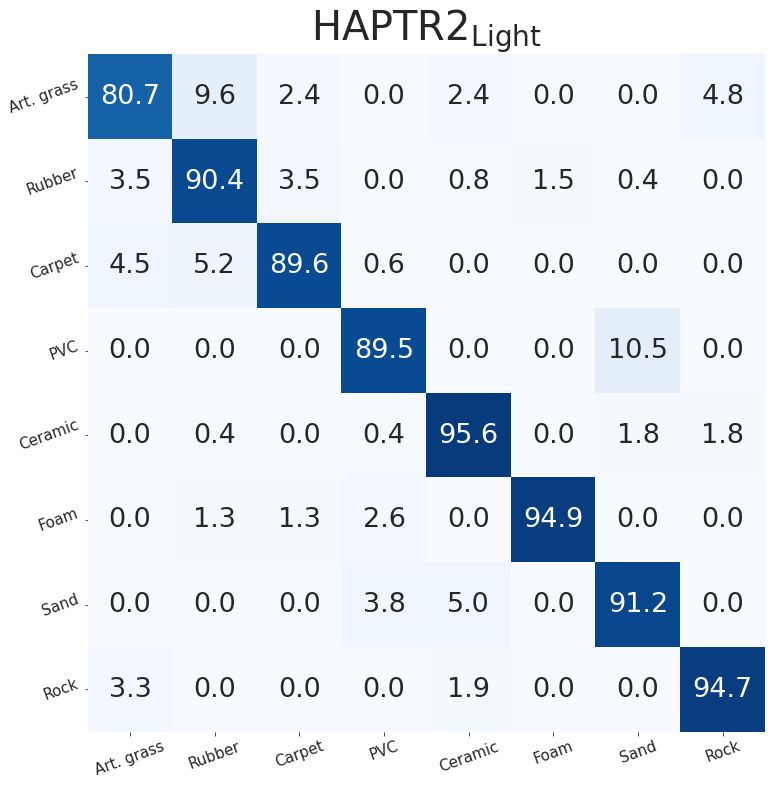
\includegraphics[width = 0.75\columnwidth]{images/transformers/haptrpp-light.png}
        \caption{\elsevier{2022} The confusion matrix presents the per-class accuracy obtained with the \acrshort{haptr}2\textsubscript{Light}.}
        \label{fig:confusion}
    \end{center}
\end{figure}

The class that caused the lowest $Acc_{min}$ for all tested deep learning models was artificial grass. One can observe that it was most often misinterpreted as the rubber -- in 9.6\% of predictions. Moreover, rubber was the most common mistake for a carpet, as the system was wrong in 5.2\% of cases. One can assume that it is due to the designed terrain -- a carpet sample was put on one slope, while squares of artificial grass lay close to the slope's beginning and end while rubber was on the second slope. That confirms that terrain recognition is more challenging in non-flat areas. There is still room for further improvements, \ie data augmentation targeting these cases or utilization of orientation sensors to incorporate information about the inclination to predictions. However, the highest classification error among all classes was made for the \acrshort{pvc} terrain incorrectly recognized as sand in 10.5\% of predictions of that class. The root cause was that both of them were neighboring each other. Hence the sand particles were present in the \acrshort{pvc} terrain, which misled the perception system. One can observe that a confusion matrix is related to the similarity between terrain and their placement on the map, which might be an informative cue in a localization task~\cite{KubaRNN}. 

\subsection{Robust robotic perception}
\label{part:experiments:terrain:robustness}

The robot operating in the real-world environment must adapt to the changing conditions that cannot be predicted and thus trained before the deployment. To achieve the desired generalization ability and robustness, the \acrshort{haptr}2\textsubscript{Light} model included the novel \acrshort{mal}. The \acrshort{mal} is responsible for dynamic adaptation of the weights of sensing modalities. This section contains the best-performing model's evaluation with and without this module to show its influence on predictions. Notably, not all modalities are equivalent. \acrshort{haptr}2\textsubscript{Light} trained exclusively on torques achieved ~88\% accuracy in the test, while trained on forces only resulted in ~60.0\%. This experiment showed that torques are \textit{leading modality} in the PUTany dataset. Nevertheless, experiments utilizing both modalities achieved the highest performance.

\begin{table}[htbp!]
    \centering
    \caption{\elsevier{2022} Classification accuracy of the \acrshort{haptr}2\textsubscript{Light} models trained with and without the additional modality attention module.}
    
    \begin{tabular}{ccccccc}
    \hline
        \acrshort{haptr}2\textsubscript{Light} & $Acc$ [\%] & $Acc_{min}$ [\%] \\ \hline
        with \acrshort{mal} & 91.7 & 80.7 (Art. grass) \\ 
        without \acrshort{mal} & 91.3 & 76.0 (Art. grass)\\ \hline
    \end{tabular}
    \label{tab:robustness_results}
\end{table} 

Firstly, as the \acrshort{mal} can work as a standalone module, its influence was verified on the overall accuracy performance. \Table~\ref{tab:robustness_results} presents the results of the \acrshort{haptr}2\textsubscript{Light} model obtained on the \acrshort{putany} test dataset with and without the \acrshort{mal}. One can observe a minor improvement in the general classification accuracy (0.4\%) due to the input modality weighting. However, the $Acc_{min}$ metric was higher by 4.7\% when the architecture included the \acrshort{mal}. That indicates that the model is more suited when training data is unbalanced.

Legged robots operate in diverse environments that can influence their sensory measurements. In most cases, operation in a novel surrounding results in inferior performance to the samples familiar to the system. The goal is to design a system that can operate despite these changes. The experiments evaluated the performance of the \acrshort{haptr} in two simulated scenarios. Initially, the robot's payload was modified, changing the forces and torque distribution. Then, a sensory failure was simulated that might occur when a mobile robot traverses harsh terrain. We mimicked these cases by adding a particular type of noise to an already normalized measurement input determined to have zero mean and a unit standard deviation. The real-world effects occurring when the robot inspects the mine tunnels equipped with conveyor belts explain using a uniform noise in this experiment. The robot experiences noise from electrical equipment and motors, which were the root of the noise on the analogue sensors.

\begin{figure}[htbp!]
    \begin{center}
        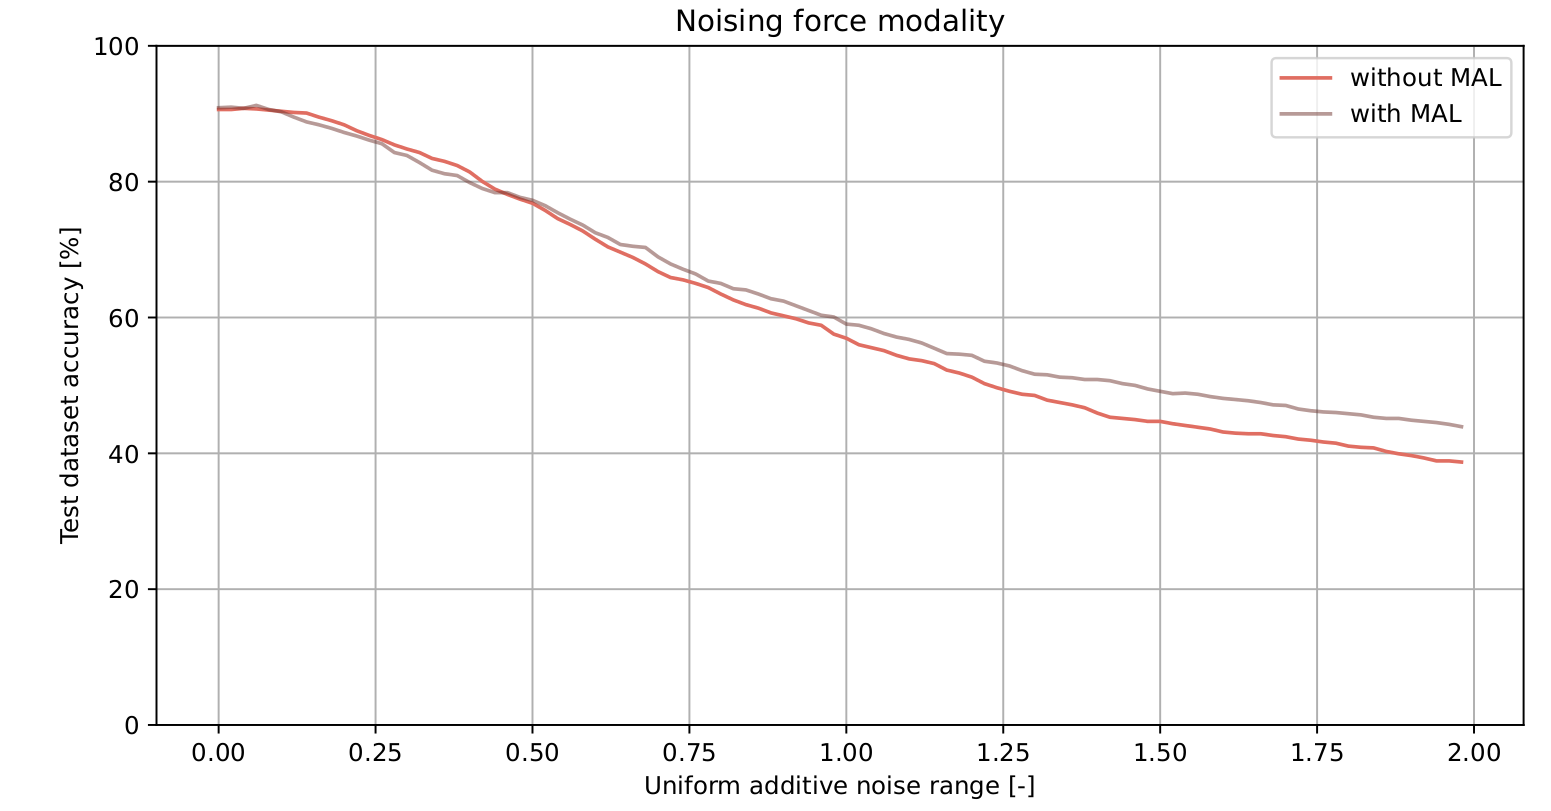
\includegraphics[width = \columnwidth]{images/transformers/robustness_increasing_payload.png}
        \caption{\elsevier{2022} The simulation of the payload changes in the \acrshort{putany} test dataset and its influence on the performance of \acrshort{haptr}\textsubscript{Light}.}
        \label{fig:robustness_bias}
    \end{center}
\end{figure}

The payload change scenario simulates an additional increase in mass by adding a bias to forces. Each step consists of a stance and a flight. An assumption is that a robot's leg swings from $60$ to $15$ degrees from the normal to the ground during the stance to simulate the payload changes. In the following procedure, a simulated payload vector acts along the gravity vector and has an increased length, influencing the network predictions more. However, it is crucial to note that payload changes would also influence the torques. Regardless, the author of the following thesis did not find any effective method to simulate this effect. Hence torques stood unchanged. Firstly, the deep learning model fit to original data, but its weights stayed frozen during the simulation. Then, the simulated payload was added to the input force signal from 0.0 to 2.0. These values correspond to the robot's weight growing from an initial weight to three times the original weight. Such substantial change is unrealistic but demonstrates the generalization capabilities of the network. \Figure~\ref{fig:robustness_bias} presents accuracy depending on the simulated increase in mass. In this simulation, the \acrshort{haptr}2\textsubscript{Light} with \acrshort{mal} achieved higher accuracy on the \acrshort{putany} dataset in a complete range of artificial payloads. Moreover, for an unexpected $3 \times$ change in weight, one can observe the drop in the accuracy by approximately $7.5\%$ when \acrshort{mal} is not used.

\begin{figure}[htbp!]
    \begin{center}
        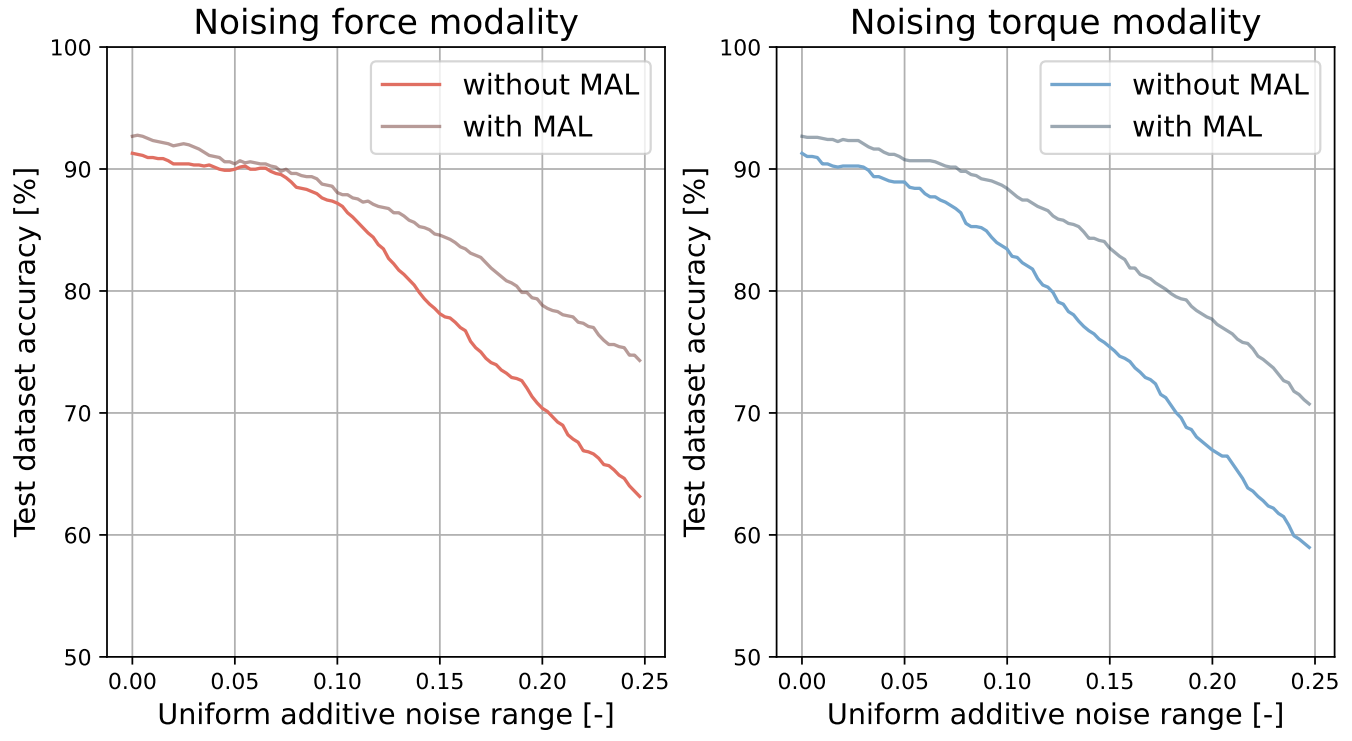
\includegraphics[width = \columnwidth]{images/transformers/robustness_increasing_noise.png}
        \caption{\elsevier{2022} HAPTR2\textsubscript{Light} accuracy on the \acrshort{putany} test dataset, in which a uniform noise with an increasing range was added to one input modality (a force or a torque) to simulate a sensor failure.}
        \label{fig:robustness_noise}
    \end{center}
\end{figure}

The simulated case of a sensory failure introduced a uniformly distributed noise from a range of 0.0 to 0.25 to sensor measurements. Like the previous scenario, the experiment investigated performance on the \acrshort{putany} dataset measuring the accuracy at different noise levels. \Figure\ref{fig:robustness_noise} shows the accuracy obtained for the data degradation scenario. As one can observe, a significant improvement in the model's robustness can be noticed for both input modalities, achieving over 10\% of accuracy improvement for the highest noise levels when it used the \acrshort{mal}. Moreover, the \acrshort{haptr} was more robust to the changes in the force measurements proving that the torque measurements might have a higher impact on the final performance of the network.

\subsection{Comparison to the state-of-the-art}
\label{part:experiments:terrain:sotacomparison}

The terrain classification algorithms for walking robots are mostly incomparable due to the different terrain types and hardware platforms. Nevertheless, it is changing due to the emergence of public datasets that facilitate impartial comparisons between methods. The results achieved were compared to the most recent method~\cite{Ahmadi2021}. In that article, the authors evaluated \acrshort{rnn}s+\acrshort{fc} on the \acrshort{putany} dataset and their \acrshort{qcat} (made publicly available). The following experiments assessed the \acrshort{haptr}2\textsubscript{Light} using the same evaluation procedure on both of these datasets using their cross-validation steps with the same data splits. \Figure\ref{tab:cross-val} presents the obtained results.

\begin{table}[htbp!]
    \centering
    \caption{\elsevier{2022} Classification accuracy of the proposed \acrshort{haptr}2\textsubscript{Light} and state-of-the-art \acrshort{rnn}s+\acrshort{fc}  measured on the \acrshort{qcat} and \acrshort{putany} datasets with the 10-fold cross-validation providing mean, standard deviation (SD), and min and max values for each fold. The best results are bolded.}
    \label{tab:cross-val}
    
    \resizebox{\columnwidth}{!}{
        \begin{tabular}{cccccc}
        \hline
        &               Dataset                    & Mean {[}\%{]} & SD {[}\%{]} & Min {[}\%{]} & Max {[}\%{]} \\ \hline
        \acrshort{haptr}2\textsubscript{Light}  & \multirow{2}{*}{PUTany}  & \textbf{93.85}         & 0.82        & 92.68        & 95.29      \\
        \acrshort{rnn}s+\acrshort{fc}~\cite{Ahmadi2021} &        & 93.20         & 0.89        & 92.06        & 95.39        \\ \hline
        \acrshort{haptr}2\textsubscript{Light}  & \multirow{2}{*}{\acrshort{qcat}}    & \textbf{97.33 }        & 1.21        & 95.49        & 98.96        \\
        \acrshort{rnn}s+\acrshort{fc}~\cite{Ahmadi2021} &        & 96.60         & 0.89        & 95.49        & 98.61        \\ \hline
        \end{tabular}
    }
\end{table}

The \acrshort{haptr}2\textsubscript{Light} outperformed \acrshort{rnn}s+\acrshort{fc} on both datasets with an accuracy margin of $0.64\%$ for \acrshort{putany} and $0.73\%$ for \acrshort{qcat} datasets. The results showed similar standard deviations, thus proving that most methods would work similarly in the real-world environment.  The \acrshort{haptr}2\textsubscript{Light} is significantly smaller comparing the number of parameters and is more suitable for deploying on a real robot than \acrshort{rnn}s+\acrshort{fc}. Using the implementation shared by the authors of~\cite{Ahmadi2021}, the \acrshort{rnn}s+\acrshort{fc} consists of 395106 trainable variables with recurrent units. In contrast, the \acrshort{haptr}2\textsubscript{Light} had only 12568 in total, which is over 30 times less. Moreover, an inference time was measured equal to 130.44~ms on a \acrshort{gpu} and 38.44~ms on a \acrshort{cpu} for the \acrshort{rnn}s+\acrshort{fc}. Similar to~\cite{KubaRNN}, the inference on a \acrshort{gpu} took longer than on a \acrshort{cpu}. \acrshort{gpu}s are preferable processing units only when we process large batches of data.  The experiments focused on the real-time robotics perspective, which prefers the inference of a single sample to reduce the delay between the measurement and the processed result.

\chapter{Robust multi-modal fusion}
\label{part:experiments:fusion}

\section{Multi-modal fusion from the robotics perspective}
\label{part:experiments:fusion:multi}

The primary objective of this section is to present the outcomes of the experiments conducted on robust multi-modal fusion with an emphasis on the robotics perspective of the problem. The following section will delve into this topic in more detail, and I urge readers to refer to \ref{part:methods:fusion:multimodal} for a comprehensive discussion on the methodology and materials used.

\subsection{Comparison of fusion methods}
\label{part:experiments:fusion:multi:comparison}

The first stage of experiments shows the performance of fusion methods on the \acrshort{bigs} dataset in the grasp outcome classification -- a success or a failure. Input modalities include gripper positions, orientations, and 3-axis forces from a wrist-mounted \acrshort{ft} sensor. \Table~\ref{tab:bigs_results} presents the final results with mean accuracy [\%] with its standard deviation among the consecutive folds. The best-performing models of Late (I-fold), \acrshort{moe} (III), \acrshort{mid} (II), and \acrshort{lmf} (I) appeared in the assessment of their robustness against data degradation and influence of input data augmentation. The fact that the average results in subsequent folds were very similar means that differences in data distributions across folds were negligible.

\begin{table}[H]
\centering
\caption{The classification accuracy comparison of four fusion methods performed on the BioTac Grasp Stability Dataset (\acrshort{bigs}) dataset.}
\begin{tabular}{ccccccc}
\toprule
\textbf{}                                                  & \textbf{I}                                                   & \textbf{II}                                                  & \textbf{III}                                                 & \textbf{IV}                 & \textbf{V}                  & \textbf{Mean}           \\ \midrule
\multicolumn{1}{c}{{\color[HTML]{000000} Late}} & \textbf{88.9}                      & {\color[HTML]{000000} 88.1}                                  & {\color[HTML]{000000} 87.9}                                  & {\color[HTML]{000000} 88.5} & {\color[HTML]{000000} 88.1} & 88.3 $\pm$ 0.4 \\ \midrule
\multicolumn{1}{c}{{\color[HTML]{000000} \acrshort{moe}}}  & \color[HTML]{000000} 89.0                                  & {\color[HTML]{000000} 88.3}                                  & {\color[HTML]{000000} \textbf{89.1}} & {\color[HTML]{000000} 87.6} & {\color[HTML]{000000} 88.4} & 88.5 $\pm$ 0.6 \\ \midrule
\multicolumn{1}{c}{{\color[HTML]{000000} \acrshort{mid}}}  & {\color[HTML]{000000} 88.1}                                  & \color[HTML]{000000} \textbf{89.9} & {\color[HTML]{000000} 89.0}                                  & {\color[HTML]{000000} 87.8} & {\color[HTML]{000000} 88.6} & 88.7 $\pm$ 0.8 \\ \midrule
\multicolumn{1}{c}{{\color[HTML]{000000} \acrshort{lmf}}}  & \color[HTML]{000000} 89.6 & {\color[HTML]{000000} 88.4}                                  & {\color[HTML]{000000} 88.0}                                  & {\color[HTML]{000000} 88.4} & {\color[HTML]{000000} \textbf{88.9}} & 88.7 $\pm$ 0.6 \\ \bottomrule
\end{tabular}  
\label{tab:bigs_results} 
\end{table}

Cross-validation on the \acrshort{hatt} dataset was another experiment step. Results in the form of the classification accuracy [\%] were reported in \Table~\ref{tab:hatt_results}. In the following scenario, there appeared time-series---a squashed 1-dimensional representation of acceleration and velocity, together with a normal force acting on a haptic device's tool-tip. For the next experiments, the II-fold models were chosen for the Late, \acrshort{moe}, \acrshort{lmf} methods, and the III-fold model for the \acrshort{mid} fusion approach.

\begin{table}[H]
\centering
\caption{The classification accuracy comparison of four fusion methods performed on the \acrshort{hatt} dataset.}
\begin{tabular}{ccccccc}
\toprule
\textbf{}                                                  & \textbf{I}                  & \textbf{II}                                                  & \textbf{III}                                                 & \textbf{IV}                 & \textbf{V}                  & \textbf{Mean}                                  \\ \midrule
\multicolumn{1}{c}{{\color[HTML]{000000} Late}} & {\color[HTML]{000000} 79.5} & \color[HTML]{000000} \textbf{80.8} & {\color[HTML]{000000} 79.4}                                  & {\color[HTML]{000000} 78.3} & {\color[HTML]{000000} 79.5} & {\color[HTML]{000000} 79.5 $\pm$ 0.9} \\ \midrule
\multicolumn{1}{c}{{\color[HTML]{000000} \acrshort{moe}}}  & {\color[HTML]{000000} 77.9} & \color[HTML]{000000} \textbf{78.9} & {\color[HTML]{000000} 74.3}                                  & {\color[HTML]{000000} 76.6} & {\color[HTML]{000000} 73.4} & {\color[HTML]{000000} 76.2 $\pm$ 2.3} \\ \midrule
\multicolumn{1}{c}{{\color[HTML]{000000} \acrshort{mid}}}  & {\color[HTML]{000000} 78.9} & {\color[HTML]{000000} 75.4}                                  & \color[HTML]{000000} \textbf{79.8} & {\color[HTML]{000000} 78.3} & {\color[HTML]{000000} 76.6} & {\color[HTML]{000000} 77.8 $\pm$ 1.8} \\ \midrule
\multicolumn{1}{c}{{\color[HTML]{000000} \acrshort{lmf}}}  & {\color[HTML]{000000} 78.1} & \color[HTML]{000000} \textbf{80.9} & {\color[HTML]{000000} 78.9}                                  & {\color[HTML]{000000} 78.3} & {\color[HTML]{000000} 79.5} & {\color[HTML]{000000} 79.1 $\pm$ 1.1} \\ \bottomrule
\end{tabular}
\label{tab:hatt_results}
\end{table}

The \acrshort{phac} dataset took part in the multi-label classification of haptic adjectives. Similarly, as in the~\cite{haptic_from_vision_and_biotac}, a performance metric was the \acrfull{auc} -- an area under the \acrfull{roc}, which is a typical performance metric used in the literature about the multi-label classification. It measures how well the predictive model can distinguish between classes (haptic adjectives). Moreover, it considers correspondences between a sensitivity/specificity ratio to multiple values of a decision threshold. Generally, \acrshort{auc}-\acrshort{roc} is a metric that gives an overall evaluation of performance, taking into account all potential classification thresholds. A common interpretation of \acrshort{auc}-\acrshort{roc} is the likelihood of the model ranking a random positive instance higher than a random negative instance. In the \acrshort{auc}-\acrshort{roc} metric, a value of 1.0 refers to an excellent classification ability, 0 means that the model is always wrong, while 0.5 means that the model has no discrimination capacity. \Table~\ref{tab:phac_results} presents the \acrshort{auc}-\acrshort{roc} metric achieved by fusion methods. Further experiments include the V-fold Late and \acrshort{moe}, I-fold \acrshort{mid}, and the IV-fold \acrshort{lmf} model.

\begin{table}[H]
\centering
\caption{The comparison of four fusion methods did on the \acrshort{phac} dataset. All values represent the \acrshort{auc}-\acrshort{roc} results.}
\begin{tabular}{ccccccc}
\toprule
\textbf{}                                                  & \textbf{I}                                                    & \textbf{II}                  & \textbf{III}                 & \textbf{IV}                                                   & \textbf{V}                                                    & \textbf{Mean}                                     \\ \midrule
\multicolumn{1}{c}{{\color[HTML]{000000} Late}} & {\color[HTML]{000000} 0.923}                                  & {\color[HTML]{000000} 0.924} & {\color[HTML]{000000} 0.922} & {\color[HTML]{000000} 0.923}                                  & \color[HTML]{000000} \textbf{0.925} & {\color[HTML]{000000} 0.923 $\pm$ 0.001} \\ \midrule
\multicolumn{1}{c}{{\color[HTML]{000000} \acrshort{moe}}}  & {\color[HTML]{000000} 0.923}                                  & {\color[HTML]{000000} 0.919} & {\color[HTML]{000000} 0.919} & {\color[HTML]{000000} 0.923}                                  &\color[HTML]{000000} \textbf{0.927} & {\color[HTML]{000000} 0.922 $\pm$ 0.003} \\ \midrule
\multicolumn{1}{c}{{\color[HTML]{000000} \acrshort{mid}}}  & \color[HTML]{000000} \textbf{0.929} & {\color[HTML]{000000} 0.922} & {\color[HTML]{000000} 0.922} & {\color[HTML]{000000} 0.927}                                  & {\color[HTML]{000000} 0.925}                                  & {\color[HTML]{000000} 0.925 $\pm$ 0.003} \\ \midrule
\multicolumn{1}{c}{{\color[HTML]{000000} \acrshort{lmf}}}  & {\color[HTML]{000000} 0.896}                                  & {\color[HTML]{000000} 0.898} & {\color[HTML]{000000} 0.902} & \color[HTML]{000000} \textbf{0.908} & {\color[HTML]{000000} 0.900}                                  & {\color[HTML]{000000} 0.901 $\pm$ 0.005} \\ \bottomrule
\end{tabular}
\label{tab:phac_results}
\end{table}
\unskip

The important note is that the primary target of the experiments was to examine methods of homo and heterogeneous signals collection. Different sets of modalities were used from each dataset, and no modality was repeated between datasets even though, \eg in the \acrshort{bigs} and \acrshort{phac}, there were used the same BioTacs tactile sensors.

The mean accuracy of all methods tested on the \acrshort{bigs} dataset was around 88\%, with insignificant differences between folds. Nevertheless, the most efficient fusion method in the grasp classification task was the \acrshort{lmf} due to a decreased standard deviation among folds than the second method - the \acrshort{mid}. Tests on the \acrshort{hatt} exhibited a slight increase of a mean results variance among different approaches and standard deviations among folds compared to \acrshort{bigs} results. The best method for texture recognition was the Late fusion, which achieved a mean test accuracy of 79.5\% between folds, additionally the least standard deviation equal to 0.9\%. In the multi-label classification of haptic adjectives based on visual and haptic data, the Late, \acrshort{moe}, and the \acrshort{mid} fusion methods were extremely close to each other in terms of a mean \acrshort{auc}-\acrshort{roc} metric, achieving a result of 0.92. The \acrshort{lmf} performance was marginally below the other. 

The results from 5-fold cross-validation and tests on separate subsets on all tested datasets showed that data used in experiments were consistent, and there were no significant outliers among folds. That finding made it possible to perform reliable experiments and ensure a fair comparison. Mean values of metrics among different fusion methods may suggest that the type of data fusion affects the efficiency only to a limited extent. When all modalities are available and free of noise, it appears that more important was a reliable data preparation (\mbox{\eg ensuring a} balanced distribution between classes in the train and test subsets, as well as between folds) for the training procedure than the fusion algorithm itself. The best-performing methods are marked with a bold font in \Table~\ref{tab:bigs_results},~\ref{tab:hatt_results}, and~\ref{tab:phac_results}. Tested neural networks were trained end-to-end and functioned moderately well, exhibiting a great capacity to learn from large (\acrshort{bigs}, \acrshort{hatt}) and small (\acrshort{phac}) datasets. Additional tests were conducted on the impact of each modality on predictions and verifying the robustness of each method against data deterioration.

\subsection{Data degradation robustness}
\label{part:experiments:fusion:multi:degradation}

The research carried out in the following section brought conclusions on the capabilities of each fusion method to translate knowledge from one modality into another and revealed that often one leading modality exists. Each dataset has a modality of vital importance for the final results. To make this dependency visible, \Figure\ref{he:bigs}--\ref{he:phac} present the results in the form of heat maps. Heat maps present changes in performance caused by the deterioration of the quality of one or more input modalities. In the following experiments, fusion methods were tested in scenarios described below, and each row in heat maps corresponds to one of the scenarios:

\begin{enumerate}
    \item N---a Gaussian Noise $N$ added to selected modalities with a 0 mean and 0.7 standard deviation;
    \item U---a uniform noise $U$ added to selected modalities that vary in the range ($-$0.5 to 0.5);
    \item 0---setting zeros in place of selected modalities, what simulated a deactivated/broken sensor; 
    \item RN---replacing selected modalities with Gaussian noise $N$, with the same parameters as $N$ from the previous scenario;
    \item RU---replacing selected modalities with uniform noise $U$, with the same parameters as $U$ from the previous scenario.
\end{enumerate}

No fixed level of noise can be considered universally unacceptable for a normalized input signal, as it depends on various factors, such as the nature of the signal, the complexity of the classifier, the performance criteria, and the tolerance level of the application. Suppose we want to determine what it means for the noise level to be significant for the chosen classifier. In that case, it is necessary to perform experiments and analyze the classifier's performance under different noise levels. Because of that, the following experiments build upon a work of~\cite{BOSS}, where the authors conducted such experiments on the relevance of noise to the time series classification on the synthetic Cylinder-Bell-Funnel dataset~\cite{saito1994local}. The authors examined the effects of Gaussian noise added to the input signal. Their results showed that the first significant drop in the classification accuracy of their baseline method happened for the Gaussian noise, with a standard deviation increasing from 0.6 to 0.7, which can be considered significant. Thus in the following experiments, the level of 0.7 was also set. In addition, unlike Gaussian noise, due to the equal probability of values across the range for homogeneous noise, its range has been reduced relative to the standard deviation of Gaussian noise. Albeit, this change relies only on the author's estimates and, to the best of the author's knowledge, has yet to be considered in the literature.

Each heat map column was annotated by a number that specified affected modalities (\mbox{\eg by the} added uniform noise). For each dataset, fusion methods were tested using three input modalities numbered as follows:

\begin{enumerate}
    \item \acrshort{bigs}---\textit{1}: gripper positions, \textit{2}: gripper spatial orientations, \textit{3}: 3-axis~force;    
    \item \acrshort{hatt}---\textit{1}: normal force, \textit{2}: squashed acceleration, \textit{3}: squashed~velocity;
    \item \acrshort{phac}---\textit{1}: images, \textit{2}: raw electrodes from the 1st sensor, \textit{3}: raw electrodes from the 2nd~sensor.
\end{enumerate}

\ Figure~\ref {he:bigs} shows heatmaps of accuracy results of selected fusion methods tested on the \acrshort{bigs} dataset. Heat maps enabled the inspection of knowledge alignment and translation of each method. In these tests, the best models from \Table~\ref{tab:bigs_results} were used.

\begin{figure}[H]
\centering
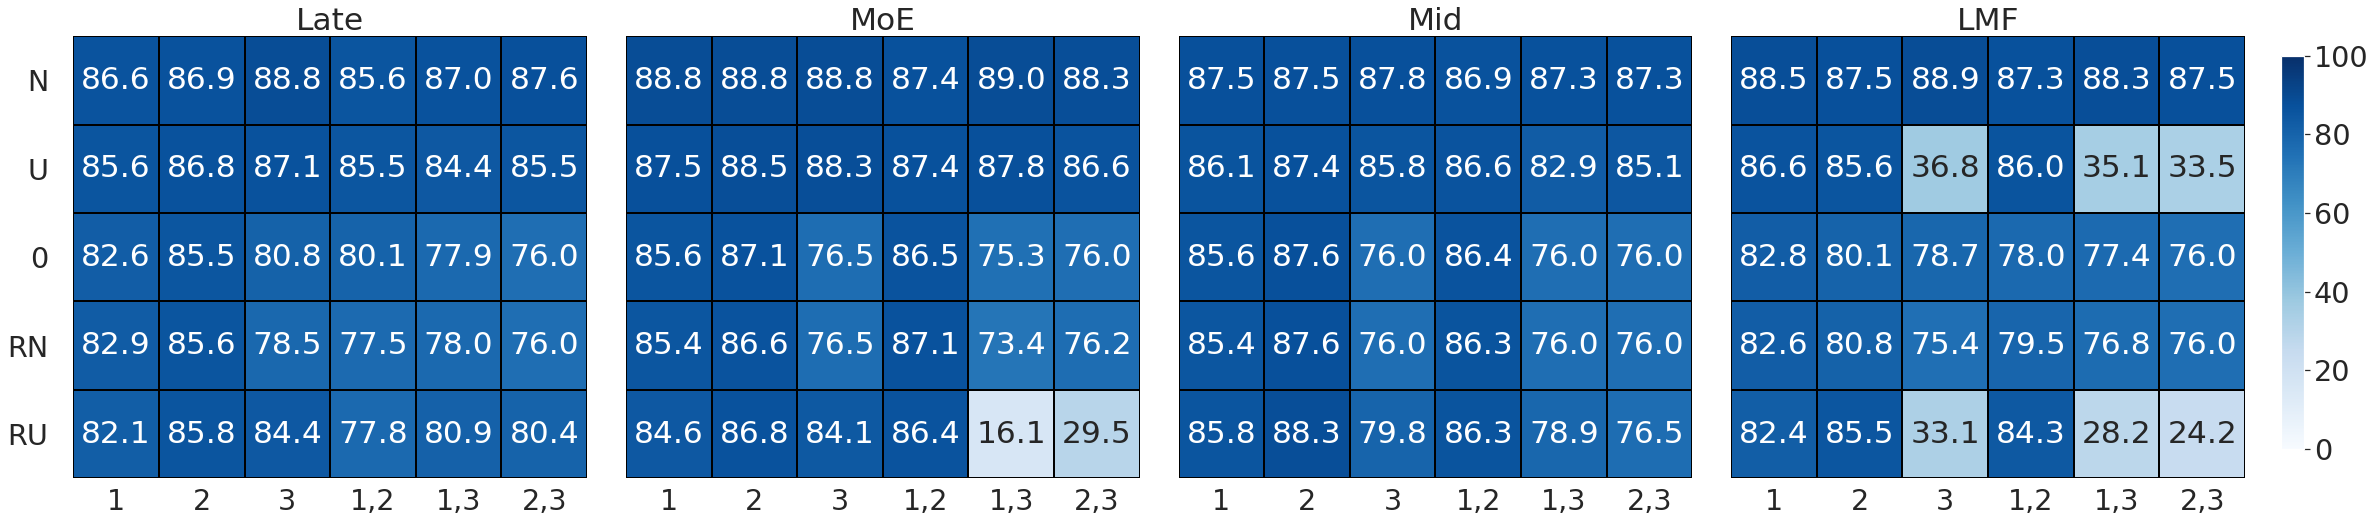
\includegraphics[width=\textwidth]{images/on_robustness/bigs_heatmaps.png}
\caption{Heat maps present results obtained by chosen models from the first stage of experiments on degraded data from the \acrshort{bigs} dataset. Classification accuracy is in [\%]. Each row corresponds to a different data degradation scenario. Columns are annotated by the indexes of affected modalities.}
\label{he:bigs}
\end{figure}   

In \Figure\ref{he:hatt}, heat maps are generated for tests on the \acrshort{hatt} dataset. The influence of each modality on the final prediction is visible, and not every method can manage data degradation. Moreover, acceleration (2nd modality) plays a leading role. It resulted in a significant deterioration of classification accuracy when noisy or faded. On the other hand, removing other modalities from the input data stream did not affect the final accuracy.

\begin{figure}[H]
\centering
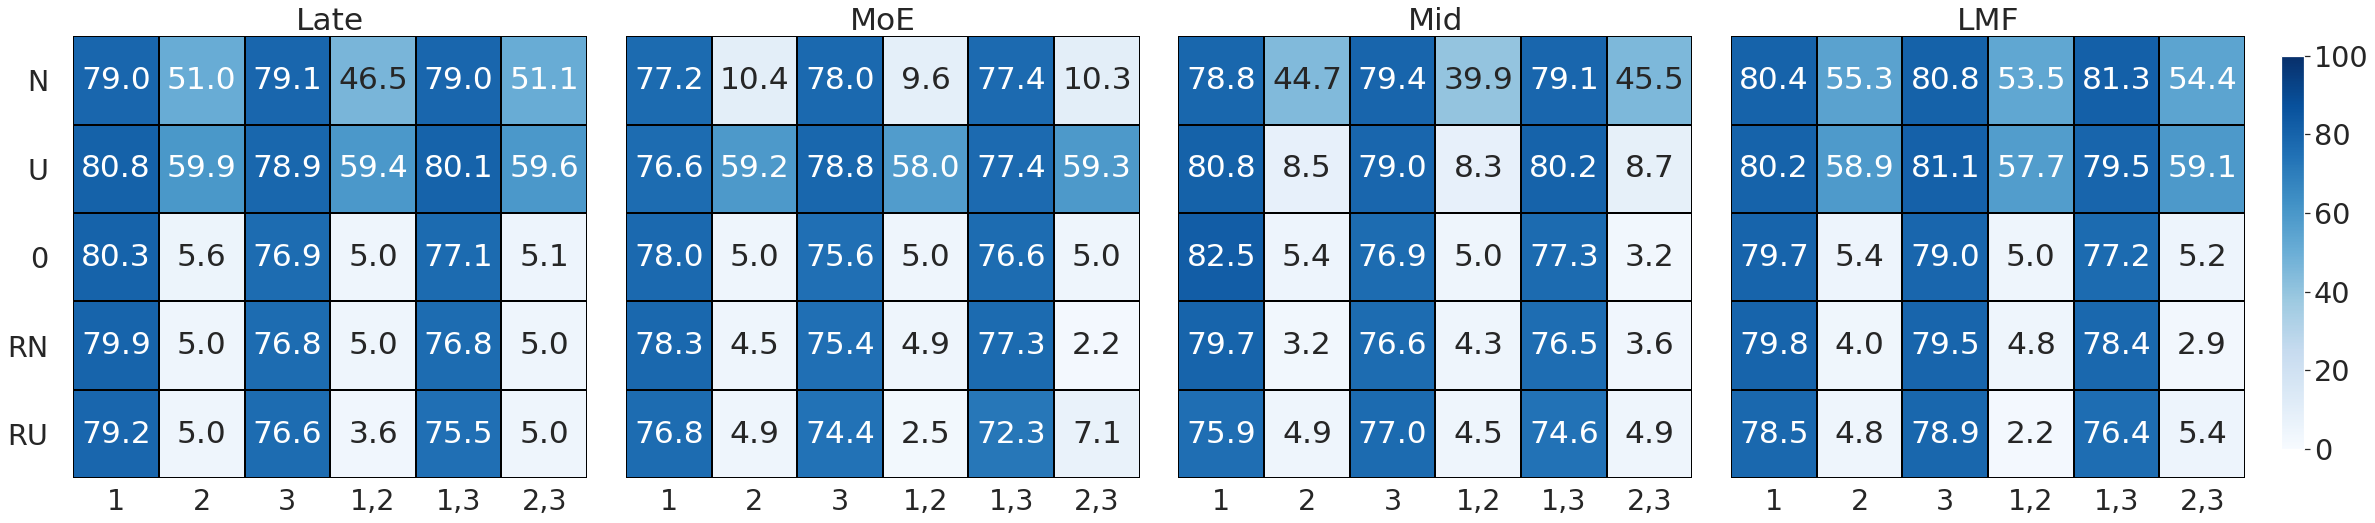
\includegraphics[width=\textwidth]{images/on_robustness/hatt_heatmaps.png}
\caption{Heat maps include the accuracy [\%] of a texture classification achieved while testing different fusion methods on degraded data from the \acrshort{hatt} dataset. Leading modality played a dominant role, which resulted in a decreased quality in case of its degradation.}
\label{he:hatt}
\end{figure} 

\Figure\ref{he:phac} reports the \acrshort{auc}-\acrshort{roc} metric for the multi-label classification of haptic adjectives. Similarly, as in the experiments on the \acrshort{hatt} dataset, the leading modality is also visible. However, its correlations with other modalities played an even more dominant role in the final performance of the methods. By inspecting heat maps, one can observe that the most meaningful correlations for predictions are between images (1st) and raw electrode signals (second and third). On the other hand, noised interactions between both electrodes' time series only slightly influenced the classification accuracy.

\begin{figure}[H]
\centering
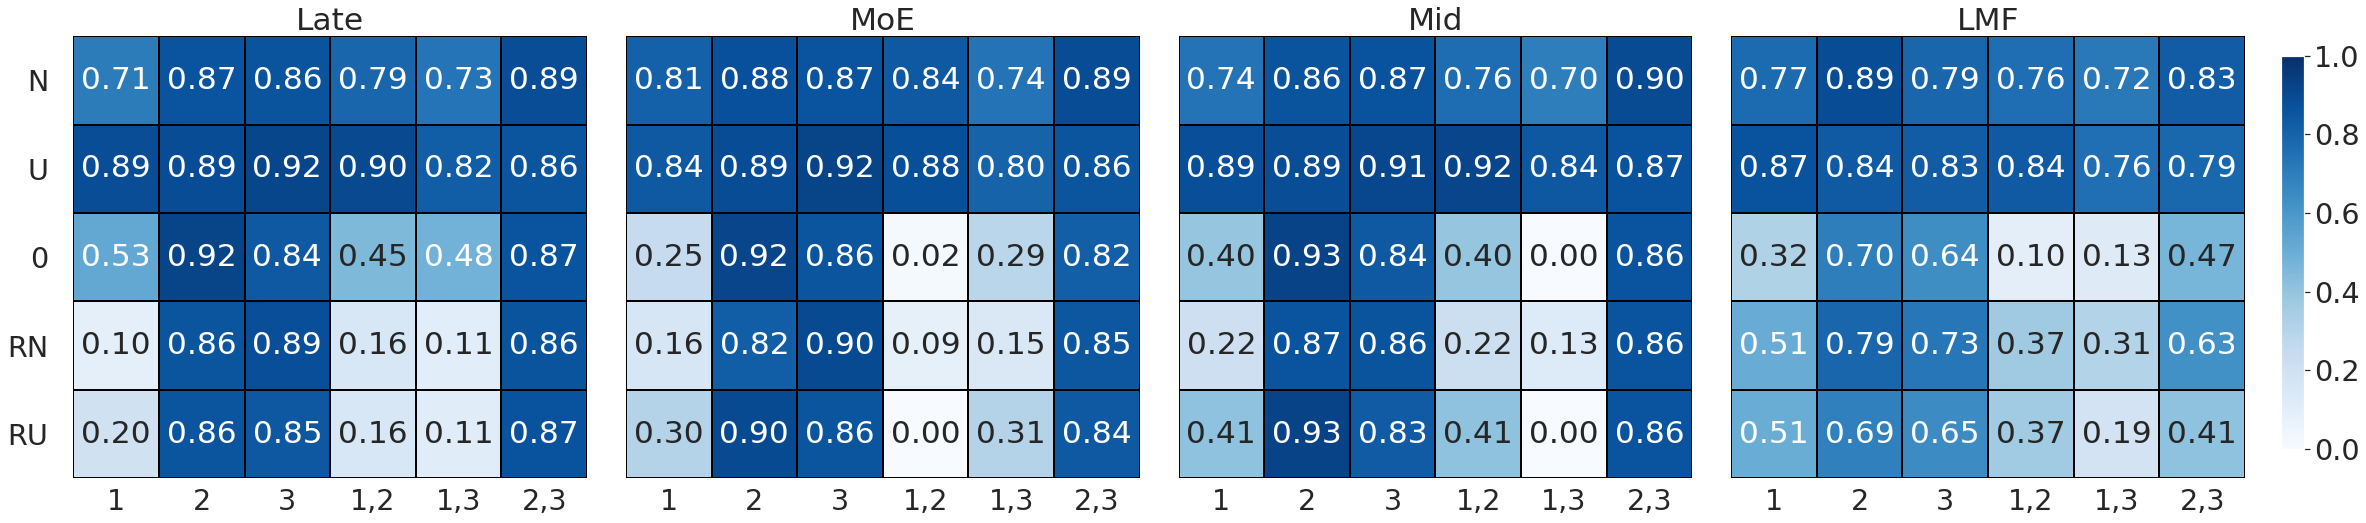
\includegraphics[width=\textwidth]{images/on_robustness/bolt_heatmaps.png}
\caption{The \acrshort{auc}-\acrshort{roc} was reported for the multi-label classification task using the \acrshort{phac} dataset. The leading modality is visible, but the correlations between modalities also affect predictions.}
\label{he:phac}
\end{figure}
\unskip 

All experiments on robustness revealed the existence of a leading modality, which means that one modality always played a dominant role in the discrimination between classes. \Figure\ref{he:bigs} presents that for the \acrshort{bigs} dataset, \acrshort{moe} and \acrshort{lmf} fusion methods exhibited significantly decreased performance when modality no. 3, which was a 3-axis force signal in combination with other modalities, was replaced by the uniform noise, and this is a leading modality in the \acrshort{bigs} dataset. The \acrshort{lmf} and \acrshort{moe} were also sensitive to the uniform noise added that affected the force signal. However, the described phenomenon did not occur for other fusion methods -- the Late and \acrshort{mid}. They appeared relatively robust for data degradation scenarios, exhibiting no more than 10\% of a drop in the accuracy when the leading modality was noised, zeroed, or replaced by noise. In the case of \acrshort{moe}, the class discrimination dropped to 16.1\% and 29.5\%. It happens because the gating network increased the importance of a leading modality for prediction. After all, it played a dominant role in providing data.

Replacing the signal with other modalities with the noise emphasized the correlation of these signals, which caused prediction errors. However, \acrshort{moe} exhibited robustness for data degradation scenarios. It appeared to be sensitive mainly to the correlations between the force signal and two other modalities -- hand positions and orientations. Similarities between modalities in the \acrshort{moe} were essential for the grasp outcome classification, not the leading modality itself. The \acrshort{lmf} method achieved close results while testing. When the uniform noise replaced the force signal, the method was more prone to mistakes, and the interactions between modalities appeared meaningless. Additionally, the \acrshort{lmf} was sensitive to scenarios that replaced the leading modality with noise and its combinations with other modalities and the noise added to the signals. This could be observed in the \acrshort{lmf} heat-map in \Figure\ref{he:bigs} looking at the results (36.8\%, 35.1\%, and 33.5\%) in the \textit{U}-row. The described phenomenon occurs because \acrshort{lmf} is a tensor-based method that highly relies on outer products between uni-modal representations inside networks. Thus the highest emphasis was put on inter-modality interactions. When finding these interactions were difficult/not possible, the \acrshort{lmf} struggled to find a correct prediction for the grasp outcome evaluation task. One can observe that the type of noise introduced to the input data played a significant role in the prediction performance because the presented findings did not repeat for a Gaussian Noise. To explain that effect, one can speculate that during the training phase, in signals, there was already some noise present similar to the normal level, which resulted in higher robustness for such a data degradation. The achieved robustness was truly substantial, and it appears that a balance between the importance of modalities was paramount. Nevertheless, verifying that relevance is very challenging and involves many experiments. 

Another dataset involved in experiments was the \acrshort{hatt}, and results gathered during that trial were reported in \Figure ~\ref{he:hatt}. Contrary to the \acrshort{bigs} dataset, one can observe that the second modality (an acceleration) caused a significant drop in the accuracy for all tested data degradation scenarios and fusion methods by inspecting heat maps. Hence, we consider acceleration to be a leading modality from the proposed set of input modalities. In the texture classification task based on haptic signals, all methods exhibited a similar performance and sensitivity to different disturbances. A lack of a legitimate acceleration signal (zeroing or replacing with a noise) always caused a decreased performance to the level of  5\% for all tested methods, which suggests that in the proposed set of modalities, the domination of acceleration was tremendous. The rest of the signals did not provide meaningful information about the process under investigation. The late fusion and \acrshort{lmf} heat-maps evaluation gave similar results for all data degradation scenarios. However, the \acrshort{moe} and \acrshort{mid} differ in terms of managing the added noise -- \acrshort{moe} exhibited sensitivity to the appearance of the noise component in the leading modality. However, the \acrshort{mid} was fragile for the same phenomenon, but with the uniform noise added. 

\Figure~\ref {he:phac} shows the results of the multi-label classification of haptic adjectives performed on the \acrshort{phac} dataset. The biggest drop in the performance metric occurred for columns missing the first modality---an image (a leading modality). In the \acrshort{moe}, the fact that the lack of images was able to cause a total failure of the classifier achieving the result of 0 (which means that the modal was always wrong) again indicates that the gating network during training put too much emphasis on the dominant modality. Considering that every result below 0.5 level means that the classifier is often wrong than right on average. The Late, \acrshort{moe}, and \acrshort{mid} methods behaved similarly across all scenarios -- the accuracy without a leading modality significantly decreased. The \acrshort{lmf} functioned slightly differently, achieving relatively good results when a noise replaced the imaging modality, which is visible in the first column of the \acrshort{lmf} heat map. However, it performed worst when other modalities were replaced by a noise/zeroed. Although it should be noted that it does not achieve 0 \acrshort{auc}-\acrshort{roc} as it happened in the case of \acrshort{moe} and \acrshort{mid}. Additionally, sometimes one can observe an improvement in the classification performance achieved when one modality was noised/faded. This phenomenon was reported, \eg for the \acrshort{mid} when the second modality (raw electrode signal) was zeroed or replaced by a uniform noise. Comparing to \Table~\ref{tab:phac_results} the improvement was 3\%.

\subsection{Data augmentation vs. leading modality}
\label{part:experiments:fusion:multi:leadingmodality}

Generated heat maps from the previous stage of experiments revealed that every dataset contains one leading modality that had the biggest impact on the prediction. In the following experiments, 33\% of randomly selected training samples of leading modalities in the training dataset were noised or faded. Half of the augmented examples were faded, and the other half noised with the 0 mean Gaussian Noise with a standard deviation of 0.7. This value should be related to the fact that the standard deviation of the data confines to 1 through data standardization. Again, The best models from previous experiments were re-trained on the same folds. \Table~\ref{tab:expIIIa} -- \ref{tab:expIIIc} presents performance of methods used in the following experiments.

Firstly, fusion models were re-trained on the augmented training dataset and tested on the same versions of the test datasets. This experiment inspected the impact of the data degradation on the performance of test sets without it. An~accuracy [\%] and \acrshort{auc}-\acrshort{roc} values [-] were presented in \Table~\ref{tab:expIIIa}. 


\begin{table}[H]
\centering

\caption{Outcomes of multi-modal fusion methods obtained for models trained on datasets containing noised/zeroed inputs from the leading modality, but~tested on the dataset without such~samples.}

\begin{tabular}{ccccc}
\toprule
\textbf{}                                    & \textbf{Late} & \textbf{\acrshort{moe}} & \textbf{\acrshort{mid}} & \textbf{\acrshort{lmf}} \\ \midrule
\multicolumn{1}{c}{\acrshort{bigs} {[}\%{]}} & 88.26         & 88.89              & 88.64        & 89.39        \\ \midrule
\multicolumn{1}{c}{\acrshort{hatt} {[}\%{]}} & 78.15         & 75.8               & 75.1         & 76.95        \\ \midrule
\multicolumn{1}{c}{\acrshort{phac}  {[}-{]}} & 0.92          & 0.93               & 0.93         & 0.91         \\ \bottomrule
\end{tabular}
\label{tab:expIIIa}
\end{table}

Secondly, they were evaluated on test datasets with the same proportion of noised samples of the leading modality without zeroed samples. \Table~\ref{tab:expIIIb} reports results obtained during that trial.

\begin{table}[H]
\centering

\caption{\Table shows results obtained for models trained on datasets containing noised/zeroed inputs from the leading modality and a noised leading modality channel during~tests.}

\begin{tabular}{ccccc}
\toprule
\textbf{}                                    & \textbf{Late} & \textbf{\acrshort{moe}} & \textbf{\acrshort{mid}} & \textbf{\acrshort{lmf}} \\ \midrule
\multicolumn{1}{c}{\acrshort{bigs} {[}\%{]}} & 88.14         & 88.64              & 88.51        & 89.26        \\ \midrule
\multicolumn{1}{c}{\acrshort{hatt} {[}\%{]}} & 65.85         & 69.95              & 65.3         & 68.3         \\ \midrule
\multicolumn{1}{c}{\acrshort{phac}  {[}-{]}} & 0.88          & 0.86               & 0.88         & 0.84         \\ \bottomrule
\end{tabular}
\label{tab:expIIIb}
\end{table}

Finally, the experiments assessed the influence of zeroed leading modalities on fusion methods in the last stage. \Table~\ref{tab:expIIIc} contains accuracy and \acrshort{auc}-\acrshort{roc} metric results gathered on the test dataset with zeroed leading modality.

\begin{table}[H]
\centering

\caption{Results obtained for models trained on datasets containing noised/zeroed inputs from the leading modality and a zeroed leading modality during tests.}

\begin{tabular}{ccccc}
\toprule
\textbf{}                                    & \textbf{Late} & \textbf{\acrshort{moe}} & \textbf{\acrshort{mid}} & \textbf{\acrshort{lmf}} \\ \midrule
\multicolumn{1}{c}{\acrshort{bigs} {[}\%{]}} & 85.77         & 88.76              & 86.27        & 89.01        \\ \midrule
\multicolumn{1}{c}{\acrshort{hatt} {[}\%{]}} & 54.85         & 57.05              & 53.95        & 53.25        \\ \midrule
\multicolumn{1}{c}{\acrshort{phac}  {[}-{]}} & 0.23          & 0.24               & 0.21         & 0.61         \\ \bottomrule
\end{tabular}
\label{tab:expIIIc}
\end{table}
\unskip

The data augmentation procedure increased robustness on noised and missing modalities for the \acrshort{bigs}. All methods gave similar results as during the tests on the data without any degradation applied on a leading modality. The proposed data augmentation procedure is sufficient to ensure robustness on noised/missing samples for the proposed input modalities. 

However, the above statement is not always true, which is visible in results obtained for the \acrshort{hatt} dataset, when the mean decrease of accuracy was from 6\% to 13\% when comparing \Table~\ref{tab:expIIIa} to \Table~\ref{tab:expIIIb} and from 18\% to 24\% between \Table~\ref{tab:expIIIa} and \ref{tab:expIIIc}. The results proved the same conclusions as before -- the leading modality in the \acrshort{hatt} dataset possessed so much information meaningful for the discrimination between textures, and other modalities played only a supporting role for that task. Nevertheless, data augmentation still brought a significant improvement in results compared to data degradation scenarios shown in \Table~\ref{he:hatt}. In both tested variants, the best-performing method was the \acrshort{moe}, which indicates that the gating network learned to refuse predictions based on a degraded leading modality.

In the multi-label classification task on the \acrshort{phac}, the Late, \acrshort{mid}, and \acrshort{moe} methods failed to assign haptic adjectives when the vision was missing. However, the \acrshort{lmf} was able to find intra- and inter-modality interactions that led to the surprisingly good result of 0.61 \acrshort{auc}-\acrshort{roc}. It indicates that the \acrshort{lmf} was the only method capable of assigning correct haptic adjectives more often than making mistakes. In tests involving noise-only samples, methods achieved similar results, and the performance metric dropped only by 4--6\%. 

\part{Conclusions}
\label{part:conclusions}

\chapter{Material recognition}
\label{part:conclusions:material}

\section{Stiffness estimation using inertial sensors}

Soft robotics solutions often take inspiration from nature, where animals exploit their flexibility to adapt to the environment, \ie a soft-bodied octopus utilizes its tentacles to grab various objects that might have complex shapes. Such an approach's key feature incorporates embodied intelligence to execute a task. However, such a method leads to troublesome control strategies and difficulties in haptic perception because there is no feedback from the soft machine, as the idea of soft robotics primarily concerns mechanical design. 

The following dissertation proposes to use contact feedback from a soft-gripper in the stiffness estimation task using \acrshort{imu}. Firstly, such an approach captures a typical inertial response of soft fingers from grasping objects of different shapes and physical parameters. Secondly, the object's physical parameters using data from \acrshort{imu} sensors is possible and beneficial due to the low cost of setup and no further need for sophisticated equipment. The deep learning solution solves the problem of grasped object stiffness estimation in soft robotics, introducing a novel approach that associates embodied and artificial intelligence. Their combination leads to a system robust to unforeseen and changing external conditions. While currently used methods of stiffness assessment exploit techniques of measurement or direct estimation, the method proposed in the dissertation characterizes the discovery of knowledge and causal relationships related to the characteristics of a given object and its physical features. Research on discovering knowledge acquired by neural networks may result in diagnosing the intuition behind humans' natural behavior in manipulating objects. It is likely that similar solutions, based on low-cost sensors and deep learning, may be successfully applied for robotic manipulation in everyday scenarios. In this work, there was published data and the implementation of neural networks used in the experiments. The author believes that it will inspire other researchers to delve into the research area of soft grippers and perception of the physical world based on tactile data in robotics.

\section{Unsupervised haptic recognition}

Although the \acrshort{dec} method outperformed other methods included in the benchmark, there is a need to mention the troubles when learning these models. Firstly, they express a high fragility on hyper-parameters, especially the batch size, which caused the learning process to collapse very early when parameter values were too high. A batch size of 256 prevents the model from learning, while a significant reduction to 16 leads to the presented results. The probable cause is the tendency of the clustering strategy to get stuck in the sharp minimum found very early in the training phase. The numerical proof for that was introduced in the following work~\cite{large_batch_bad}. The same applies to the learning rate, but the explanation is more straightforward and well-known - a too-large learning rate would cause the model to update its weights with a too-large step resulting in a deterioration of the training quality.

Moreover, experiments show that the Touching dataset was improperly designed for the considered task. As stated before, such a system's training procedure might be fragile and sensitive to the hyper-parameters choice. Any additional noise introduced in the input signals might destroy the learning curve. The situation in which different signals exhibit some false features, like, \eg the high hardness of the soft object, because the sensor sensed the hard ground beneath them, might influence the training. That phenomenon caused poor results in these experiments.

The following benchmark also presented results from other clustering methods. The conclusion is equal for all of them - they do not apply to such a task. As haptic signals are transmitted through touch, they also might be ambiguous (different objects might feel the same). It is hard to interpret what it means to be "similar" because of their multi-dimensionality and complexity. Moreover, they might depend on the interaction type: different pressure applied when touching, velocity, slippage, or temperature. All these factors significantly complicate the clustering process and exceed the abilities of the classical methods. 

Latent representations are commonly used in robotics to represent high-dimensional signals in a lower-dimensional space, making it easier for algorithms to process and understand. Additionally, using latent representation can help models generalize their knowledge and perform tasks in new environments without needing to be explicitly trained. Experiments in the chapter \ref{part:experiments:materials:unsupervised} show a slight improvement in the clustering performance between \acrshort{dec} methods working on raw data and latent vectors. On the other hand, using a \acrshort{svd} to preprocess signals for the classical approaches did not let them achieve comparable results.

Additionally, silhouette tests suggest that the optimal number of clusters is three. Considering that these experiments were targeted to prove or refute the existence of five tactile dimensions, one could summarize that they denied them, as there should be five of them as well. However, under the skin of a human's fingertip, an estimated 3000 touch receptors ensure deep and precise haptic sensing. On the other hand, even such an advanced touch sensor as BioTac has only 24 electrodes that measure temperature and tactile feedback. The \acrshort{bigs2} dataset included recordings from three such sensors, which results in 72 electrodes sensing the object at each grip. Even that might be insufficient to fully recreate the sense of touch in how humans perceive it. Presumably, sparse electrodes do not allow for adequate recognition of the macro and roughness of touched objects. However, there is no evidence that the rest of the tactile dimensions, \ie temperature, hardness, and friction, cannot be sensed using these sensors. To conclude, the silhouette test partially proved the existence of tactile dimensions. 

However, there is still room for improvement of sensors and algorithms to ensure accurate and robust haptic perception for a high-level understanding of touched objects and dexterous manipulation. This topic had an exploratory nature. The obtained results are an excellent starting point for further development during post-doctoral research.

\chapter{Terrain recognition}
\label{part:conclusions:terrain}

\section{State of the art Haptic Transformer} 

Terrain classification is one of the most prevalent features of the robotic perception system of a walking machine. The proper recognition enables a successful gait adaptation and lets the robot avoid terrains that are too hazardous to traverse. However, such a system cannot be too computationally exhaustive because a typical onboard computer has limited resources.

The \acrshort{haptr} and \acrshort{haptr}2 are novel methods for terrain classification with transformer neural networks. The attention was put on the real-world applicability and compared our approach with multiple data-driven methods, including adapted non-deep learning (\acrshort{knn}-\acrshort{dtw}, \acrshort{rocket}) and deep learning models (\acrshort{tcn}, \acrshort{cnn}-\acrshort{rnn}). The presented comparison took into account the accuracy of each method, the number of learnable parameters, and the inference time. Tests revealed that the \acrshort{haptr}2 provides the best trade-off between the accuracy and the number of parameters directly impacting inference time. Moreover, the inference time of state-of-the-art \acrshort{cnn}-\acrshort{rnn} takes too long to be applied on a real robot proving the need for broader evaluation than direct accuracy measurement. 

\section{Improved robustness of a perception system} 

Additionally, the following work focused on the robustness of robotic perception systems and introduced the \acrshort{mal} in \acrshort{haptr}2. By assigning weights to entire modalities (\acrshort{ft}, inertial sensor readings) using the dot product attention layer, the model self-attended to relevant parts of an input data stream. It resulted in increased robustness of the perception system against payload changes and deterioration of signal quality. However, the \acrshort{mal} was implemented as a universal, standalone module that could assign weights to any user-defined modalities, creating new opportunities for future research. Afterward, to establish a fair comparison with the current state of the art, the \acrshort{haptr}2 was examined using the \acrshort{qcat} dataset. The results showed that the \acrshort{haptr}2 outperformed the complex \acrshort{rnn}s+\acrshort{fc} approach~\cite{Ahmadi2021} considering accuracy and inference time performance while having over 30$\times$ less learnable parameters.

Eventually, the findings from the following dissertation were also reflected in the most up-to-date literature on the topic and fit in with existing trends in time series recognition. The usage of convolutions together with attention modules was justified in the theoretical work~\cite{park2022how}, while similar ideas regarding transformers for time-series present concurrent study presented in~\cite{TST}. 

\chapter{Robust multi-modal fusion}
\label{part:conclusions:fusion}
 
\section{Heterogeneous data fusion}
 
Typically, the more complex assignment required from the robot, the more sophisticated its perception system. For example, a robot that must detect an object in the scene and apply a specified control strategy for a pick-and-place task might require data from multiple modalities sequentially -- visual detection and haptic manipulation. However, looking at both parts of the mentioned task, each can be split into more steps. A visual approach might utilize \acrshort{rgb} images, point clouds, multispectral images, or thermal images. Haptic manipulation would need to process \acrshort{ft} signals, inertial feedback, or highly sophisticated sensory feedback from modern haptic sensors such as GelSight or BioTac. One can observe that using many modalities at once might be troublesome, as the data often is not homogeneous, thus requiring different methods to process them. The experimental verification focused on three tasks: a grasp outcome prediction, texture recognition, and multi-label classification of haptic adjectives.

The following work compares four state-of-the-art fusion methods with further analysis of obtained outcomes. It analyzes the existence and influence of the performance of so-called leading modalities. In the experiments, one modality always had a superior impact on obtained results. Because of that fact, the quality of selected methods decreased when that modality was noised or zeroed, and deep neural networks were prone to overfit these modalities. 

\section{Data degradation robustness}

The experiments examined fusion methods in possible scenarios of input data degradation that might occur in real life, \eg a sensor turn-off or measurement noise. Finally, the influence of the data augmentation technique on the predictive capabilities of tested methods was tested and again evaluated their robustness on noise added to the leading modality and its zeroing. To build reliable autonomous systems, we must focus more on the robustness of our data fusion methods introducing adaptive behavior in the data deterioration scenario. A solution for such a problem would be the \acrshort{mal} presented in the following dissertation built on top of attention modules.

\chapter{Final remarks}
\label{part:conclusions:remarks}

\section{Note from the author}

Throughout my Ph.D., I have significantly contributed to robotics and artificial intelligence, aiming at haptic perception for manipulators and walking robots. My research's most important scientific achievements include the publication of datasets and the implementation of novel neural networks that enable embodied and artificial intelligence to estimate the stiffness of materials using inertial sensors. This connection was a novelty in soft robotics because the field primarily focused on machines' mechanical design, not the algorithms themselves. Additionally, I have proved tactile dimensions in haptic data using novel and open-source datasets, which constitutes a sound introduction to the further development of touch recognition systems in an unsupervised manner, which is still a heavily underestimated topic in the literature. I have also introduced a novel deep learning method for the terrain classification of a walking robot, which uses attention layers to improve performance compared to traditional methods and other deep learning models. The proposed method utilizes inter and intra-modalities relationships to push further the accuracy of the classifier and improve its robustness against the noise. Weights produced by the attention layer might directly indicate the importance of the modalities of the multi-dimensional signal, improving the method's interpretability. Finally, I have thoroughly evaluated noise types and other degradation scenarios in time series classification using deep neural networks. This contribution is a crucial step toward developing more robust and accurate models, and my research improved the existing state of the art. These achievements would be incomplete if I did not embed them among existing solutions to the problems raised. In this way, my work's scientific value can support other researchers in their work.

However, in addition to the work presented here, I have also contributed to the field through presentations of my work and that of my colleagues at the Institute of Robotics and Machine Intelligence, both locally and globally. I was a co-author of the work "What am I touching? Learning to classify terrain via haptic sensing"~\cite{bednarek2019icra} at the prestigious International Conference on Robotics and Automation held in Montreal (ICRA, 2019) and "Robotic touch: Classification of materials for manipulation and walking"~\cite{bednarek19} at the International Conference on Soft Robotics held in Seoul (RoboSoft, 2019). Furthermore, throughout my Ph.D., I have worked as a researcher in multiple scientific projects in the field of robotics at the national and international levels, including

\begin{itemize}
    \item subTerranean Haptic INvestiGator (THING, Horizon 2020): This project aimed to improve a perception system for robotic exploration of subterranean environments. I contributed to the design and implementation of the terrain classification methods, as well as the analysis of the data.
    
    \item Robotic tEchnologies for the Manipulation of cOmplex DeformablE Linear objects (REMODEL, Horizon 2020): This project focused on developing novel robotic technologies to manipulate deformable linear objects, such as cables and wires. I worked on algorithms utilizing prototypes of novel haptic sensors.
    
    \item Perception and control in a robotic task manipulation of flexible objects (LIDER program by The National Centre for Research and Development in Poland): This project aimed to improve the perception and control of manipulators in tasks involving flexible objects. I contributed to the development and testing of the algorithms and the analysis of the results.
\end{itemize}

I also did an internship at the École Polytechnique Fédérale de Lausanne (EPFL), where I was a part of the prominent Biorobotics Laboratory (BioRob) and worked on haptic classification using a quadrupedal robot. Collaborating with researchers from various countries and universities, including Eidgenössische Technische Hochschule Zürich (ETH), EPFL, the University of Edinburgh, and Oxford University, has provided me with unique experiences and invaluable opportunities for growth and development in my research skills. 

Overall, my Ph.D. experience has provided me with diverse and challenging research opportunities and valuable collaborations with leading researchers in the field. These experiences have prepared me well for a successful robotics research and development career.

\section{List of publications}

When writing the following thesis, I authored and co-authored 15 scientific articles on robotics at international conferences and in scientific journals. My publications reached 60 citations according to the Scopus database, reaching an h-index equal to 5 and 96 citations according to Google Scholar, yielding an h-index equal to 6.

\begin{enumerate}
    \item HAPTR2: Improved Haptic Transformer for Legged Robots’ Terrain Classification – M. Bednarek, M. R. Nowicki, K. Walas, Robotics and Autonomous Systems – Selected papers from the 10th European Conference on Mobile Robots, 2022 (IF 2022: 3.7)

    \item Fast Haptic Terrain Classification for Legged Robots Using Transformer – M. Bednarek, M. Łysakowski, J. Bednarek, M. R. Nowicki, and K. Walas, European Conference on Mobile Robots, 2021

    \item Tell me, what do you see? - interpretable classification of wiring harness branches with deep neural networks - P. Kicki, M. Bednarek, P. Lembicz, G. Mierzwiak, A. Szymko, M. Kraft, \& K. Walas, Sensors Journal, 2021 (IF 2021: 3.847)

    \item Gaining a Sense of Touch Object Stiffness Estimation Using a Soft Gripper and Neural Networks – M. Bednarek, P. Kicki, J. Bednarek, K. Walas, Electronics Journal, 2021 (IF 2021: 2.690)

    \item On Robustness of Multi-Modal Fusion—Robotics Perspective – M. Bednarek, P. Kicki, K. Walas, Electronics Journal, 2020 (IF 2021: 2.690)

    \item Comparative Assessment of Reinforcement Learning Algorithms in the Task of Robotic Manipulation of Deformable Linear Objects – M. Bednarek, K. Walas, International Conference on Robotics and Automation Engineering (ICRAE), Singapore 2019

    \item Robotic Manipulation of Elongated and Elastic Objects, P. Kicki, M. Bednarek, K. Walas, Signal Processing: Algorithms, Architectures, Arrangements, and Applications, Poznan 2019

    \item What am I touching? Learning to classify terrain via haptic sensing – J. Bednarek, M. Bednarek, L. Wellhausen, M. Hutter, K. Walas, International Conference on Robotics and Automation (ICRA), Montreal 2019

    \item Robotic Touch: Classification of Materials for Manipulation and Walking, J. Bednarek, M. Bednarek, P. Kicki, K. Walas, International Conference on Soft Robotics, Seoul 2019

    \item Measuring Bending Angle and Hallucinating Shape of Elongated Deformable Objects – P. Kicki, M. Bednarek, K. Walas, Humanoids, Beijing 2019

    \item Spatial Transformations in Deep Neural Networks – M. Bednarek, K. Walas, Signal Processing: Algorithms, Architectures, Arrangements, and Applications, Poznan 2018

    \item Simulated Local Deformation \& Focal Length Optimisation for Improved Template- Based Non-Rigid Object 3D Reconstruction – M. Bednarek, K. Walas, Signal Processing: Algorithms, Architectures, Arrangements, and Applications, Poznan 2018

    \item Methods of Enriching the Flow of Information in The Real-Time Semantic Segmentation Using Deep Neural Networks – J. Bednarek, K. Piaskowski, M. Bednarek, Signal Processing: Algorithms, Architectures, Arrangements, and Applications, Poznan 2018

    \item Local Descriptors Robust to Out-of-Plane Rotations – M. Bednarek, K. Walas, Signal Processing: Algorithms, Architectures, Arrangements, and Applications, Poznan 2017

    \item Comparison of Visual Descriptors for 3D Reconstruction of Non-Rigid Planar Surfaces – M. Bednarek, International Conference on Image Processing \& Communications, Bydgoszcz 2017
    
\end{enumerate}

\bibliographystyle{IEEEtran}
\bibliography{bib}

\end{document}
